%%%%%%%%%%%%%%%%%%%%%%%%%%%%%%%%%%%%%%%%%%%%%%%%%%%%%
\chapter{Risultati e discussione}\label{ch:risultati}

In questo capitolo viene mostrato il lavoro centrale di questa tesi. Più in particolare verrà mostrata la metodologia utilizzata nel contesto di lavoro di \ttbox{PYTHIA 8.3}, ossia come  viene impostata la generazione gli eventi.
Successivamente verranno mostrati il confronto dei dati sperimentali di ALICE con le simulazioni, quali sono i contributi maggiori dei canali di produzione dei (anti)deuteroni e il confronto tra il modello di coalescenza e il modello di sezioni d'urto efficaci.
Dopodiché verrà mostrato come è stata effettuata l'ottimizzazione dei parametri di simulazione, cercando di ripercorrere le modalità utilizzate per la ricerca del parametro ottimale.
Infine si esegue un confronto delle simulazioni con il modello predefinito e il modello ottimizzato.

%%%%%%%%%%%%%%%%%%%%%%%%%%%%%%%%%
\section{La generazione degli eventi}\label{ch:settings}
Per la produzione delle simulazioni sono stati generati 98 milioni di eventi.
% NJ qui si può considerare la notazione scientifica e dire 10e8, sono sempre 98 milioni? 
Per ogni evento si sono impostate le seguenti opzioni:
\begin{itemize}
    \item ogni evento è una collisione $pp$ con l'energia del centro di massa $\sqrt{s} = 13$ TeV;
    \item si è attivata la simulazione della posizione di vertici per i partoni \\ (\ttbox{PartonVertex:setVertex = on});
    \item si è attivata la generazione di vertici nella frammentazione, ossia la formazione di particelle a partire da partoni (\ttbox{Fragmentation:setVertices = on});
    \item si è applicato un particolare \textit{tuning} (ottimizzazione) dei parametri per la simulazione delle collisioni $pp$ (\ttbox{Tune:pp = 4}, con "4" che si riferisce a un set specifico di parametri ottimizzati per certe condizioni sperimentali);
    \item si sono disattivati i sottoprocessi che coinvolgono interazioni QCD con trasferimento di momento elevato (\ttbox{HardQCD:all = off});
    \item si sono disattivati anche i sottoprocessi che coinvolgono interazioni QCD con trasferimento di momento più piccolo (\ttbox{LowEnergyQCD:all = off});
    \item si sono abilitate le interazioni QCD soft inelastiche che sono sottoprocessi di bassa energia (\ttbox{SoftQCD:inelastic = on});
    \item si è attivata la produzione di deuteroni (\ttbox{HadronLevel:DeuteronProduction = on}).
\end{itemize}
In ogni evento vengono prodotte un certo numero di particelle, che possono includere protoni, neutroni, fotoni, deuteroni e altro, con le rispettive antiparticelle, e sono stati ottenuti gli spettri di produzione di (anti)protoni e (anti)deuteroni in funzione dell'impulso trasverso $p_t$, scartando le particelle con alta pseudo-rapidità (quindi se una particella possiede pseudo-rapidità $\eta > 0.5$, essa viene scartata).
% NJ Qui il taglio era su eta o y? Dovrebbe esser y 
Inoltre si è andato a osservare gli spettri dei deuteroni in funzione della quantità di moto trasversa nei vari canali di produzione.
Contestualmente all'esecuzione di \pythiaa{}, il riempimento degli istogrammi è stato effettuato tramite l'utilizzo del programma \ttbox{ROOT} sviluppato al CERN \cite{fons_rademakers_2020_3895855}.
%%%%%%%%%%%%%%%%%%%%%%%%%%%%%%%%%%%%%%%%%%%%
\section{Risultati con parametri predefiniti}\label{ch:default}
Come già anticipato nella \autoref{ch:pythia_deuteron}, un parametro importante nella produzione deuteronica è \ttbox{norm}, che nel caso predefinito assume il valore di 119.6.
Tuttavia questo valore è stato ottenuto considerando l'energia iniziale del centro di massa a $\sqrt{s} = 7$ TeV, a differenza del valore di $\sqrt s = 13$ TeV considerato in questa tesi.
Perciò è lecito aspettarsi, a partire da questa considerazione, che vi sia una discrepanza nella produzione di (anti)deuteroni tra le simulazioni e i dati reali.
Per confrontare i dati delle simulazioni con i dati sperimentali si sono considerate le misure effettuate da ALICE riguardanti collisioni $pp$ a rapidità centrali ($|y|<0.5$) con energia del centro di massa $\sqrt s = 13$ TeV.
I dati dei protoni e dei (anti)deuteroni utilizzati in questa tesi sono tratti rispettivamente da \cite{ALICE:2020jsh} e da \cite{ALICE:2020foi}.\\

\begin{figure}[htb]
    \centering
    \begin{subfigure}{.49\textwidth}
    \centering
        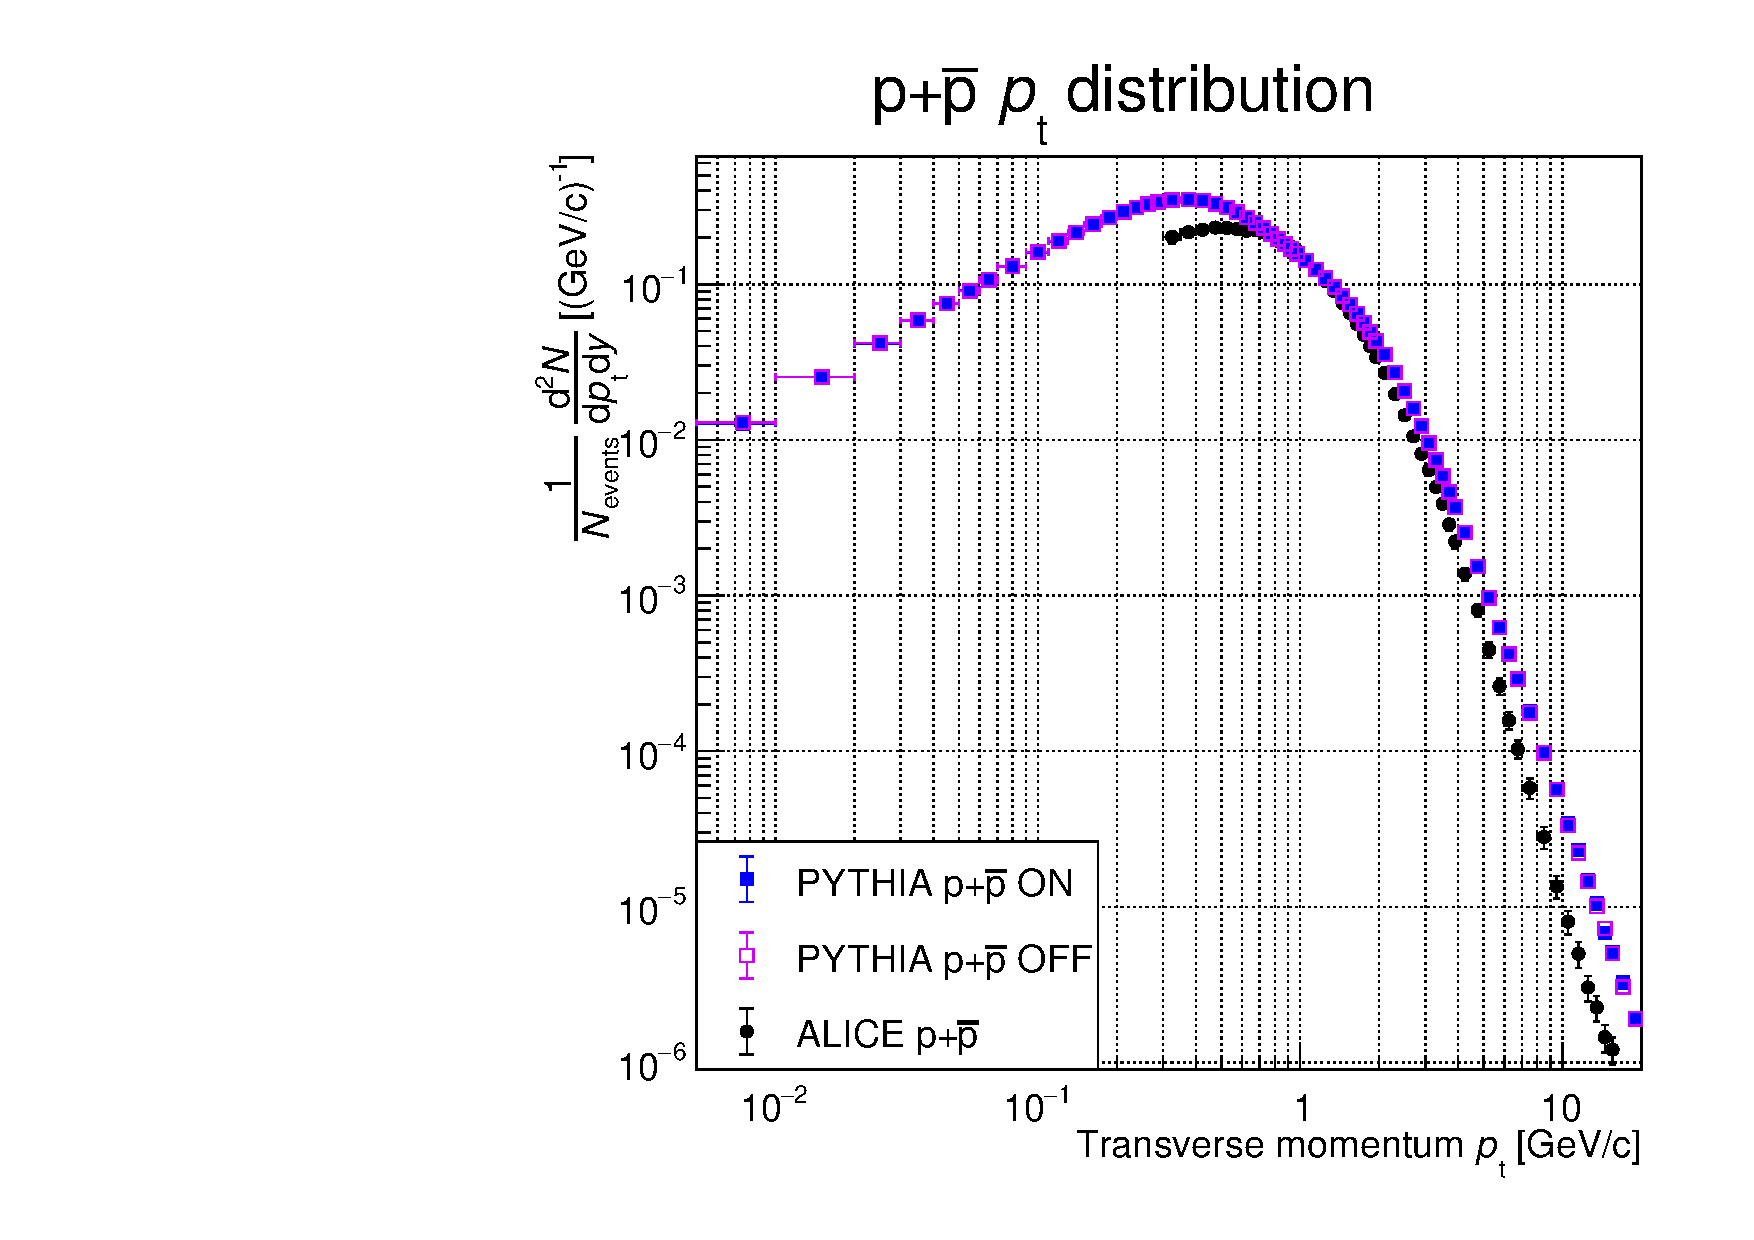
\includegraphics[width=\textwidth]{image/3-risultati/analyse/A/pp.pdf}
        \caption{}
        \label{fig:A_pp}
    \end{subfigure}
    %\hspace{1cm}
    \begin{subfigure}{.49\textwidth}
        \centering
        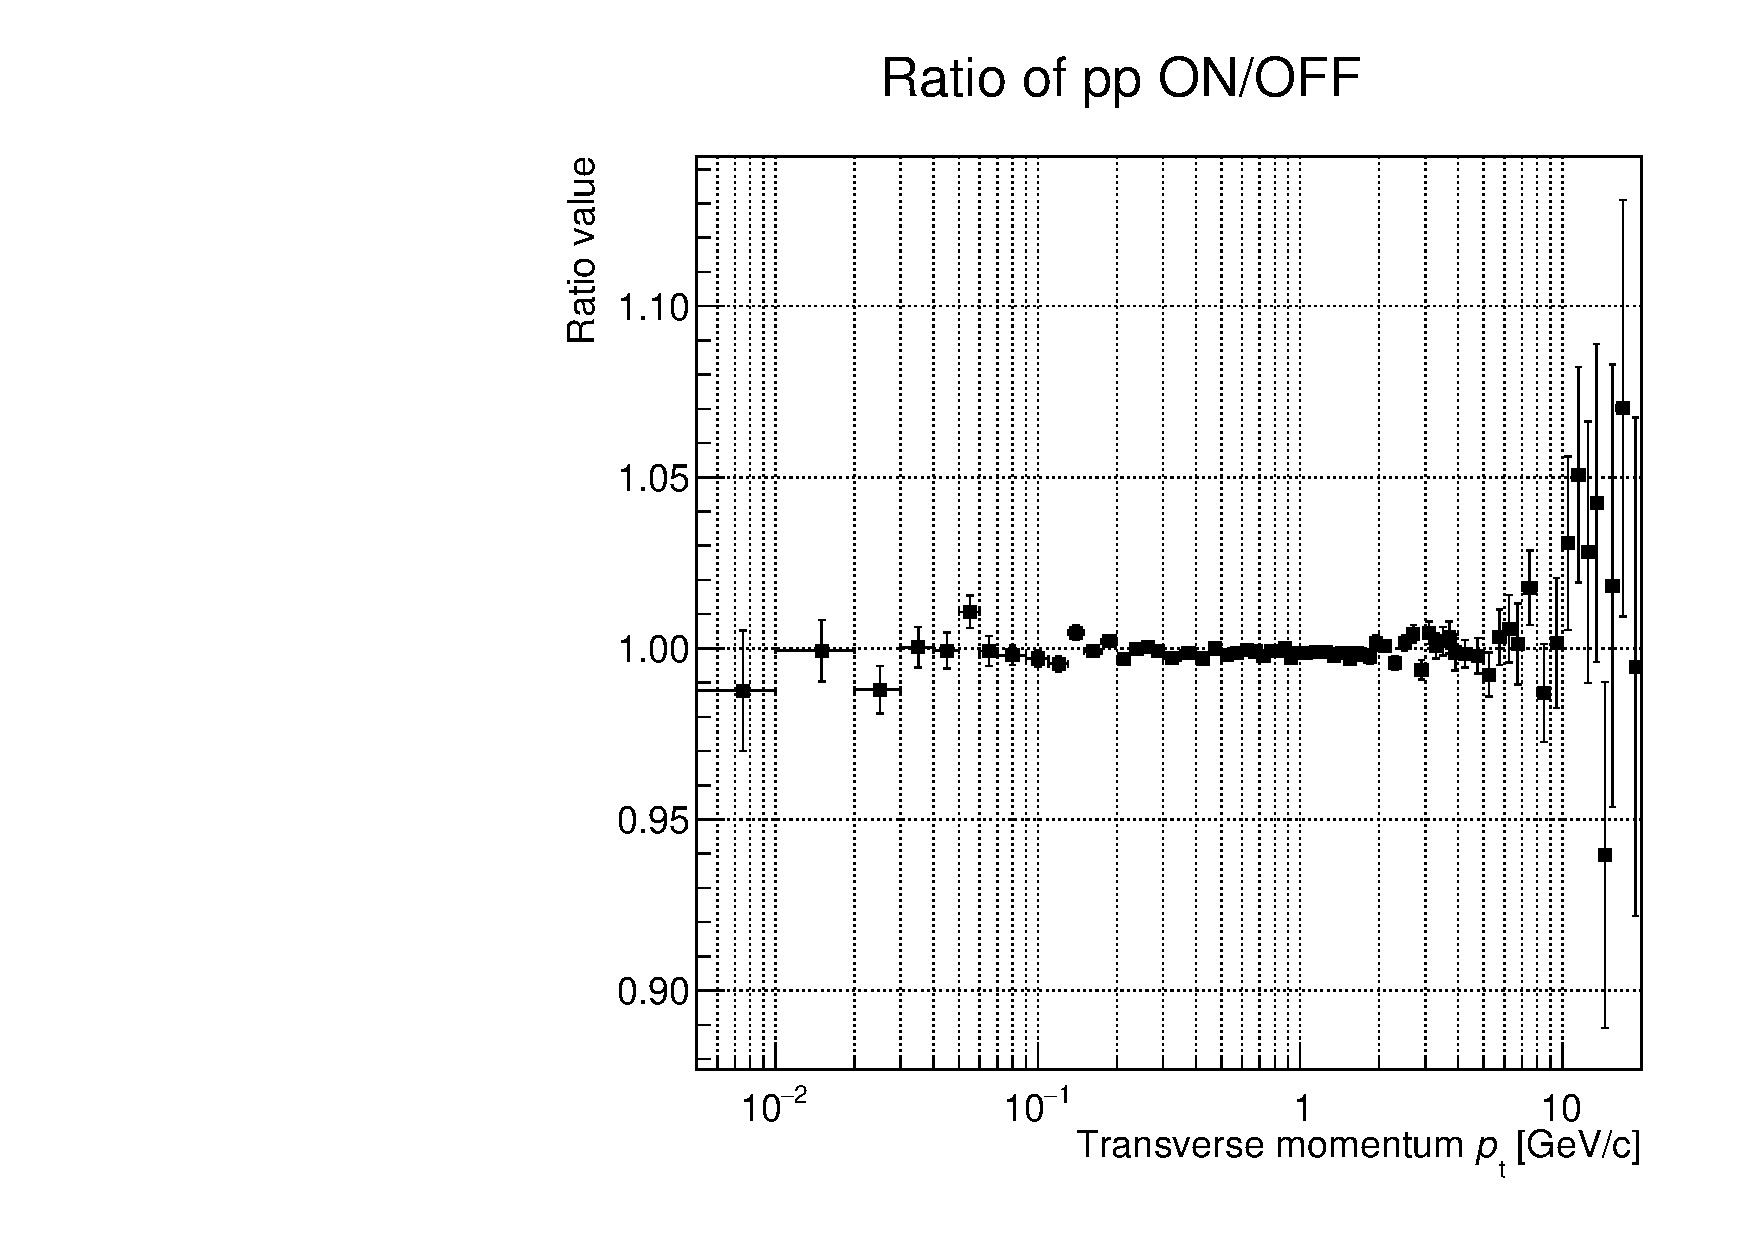
\includegraphics[width=\textwidth]{image/3-risultati/analyse/A/ratio_pp_ON_OFF.pdf}
        \caption{}
        \label{fig:A_ratio_pp_ON_OFF}
    \end{subfigure}
    \captionwithsource{\emph{\rmfamily (a)} Distribuzione dell'impulso trasverso di $p+\bar p$ con produzione deuteronica attivata e disattivata ("ON" e "OFF") in confronto con i dati sperimentali di ALICE ("ALICE"). \emph{\rmfamily (b)} Frazione della distribuzione dell'impulso trasverso di $p+\bar p$ con produzione deuteronica attivata e con produzione non attivata.}{\cite{ALICE:2020jsh}}
    \label{fig:A_pp_prod}
\end{figure}
Eseguendo la simulazione una volta con i parametri predefiniti e una volta con la produzione deuteronica disattivata (\ttbox{HadronLevel:DeuteronProduction = off}), otteniamo i vari spettri di produzione.
Ci si aspetta una piccola differenza tra il caso in cui la produzione di deuteroni è attivata e non, in particolare il numero di protoni dovrebbe essere leggermente minore in cui la produzione si attivata, visto che una parte di questi si ricombina per formare un deuterone.
Dalla \autoref{ch:objectives_alice} sappiamo che il numero di deuteroni prodotti deve essere circa 1000 volte inferiore al numero di protoni, per cui il rapporto tra numero di protoni con produzione (anti)deuteronica attivata e disattivata dovrebbe avvicinarsi al valore di 0.999.
\begin{figure}[htb]
    \centering
    \begin{subfigure}{.49\textwidth}
    \centering
        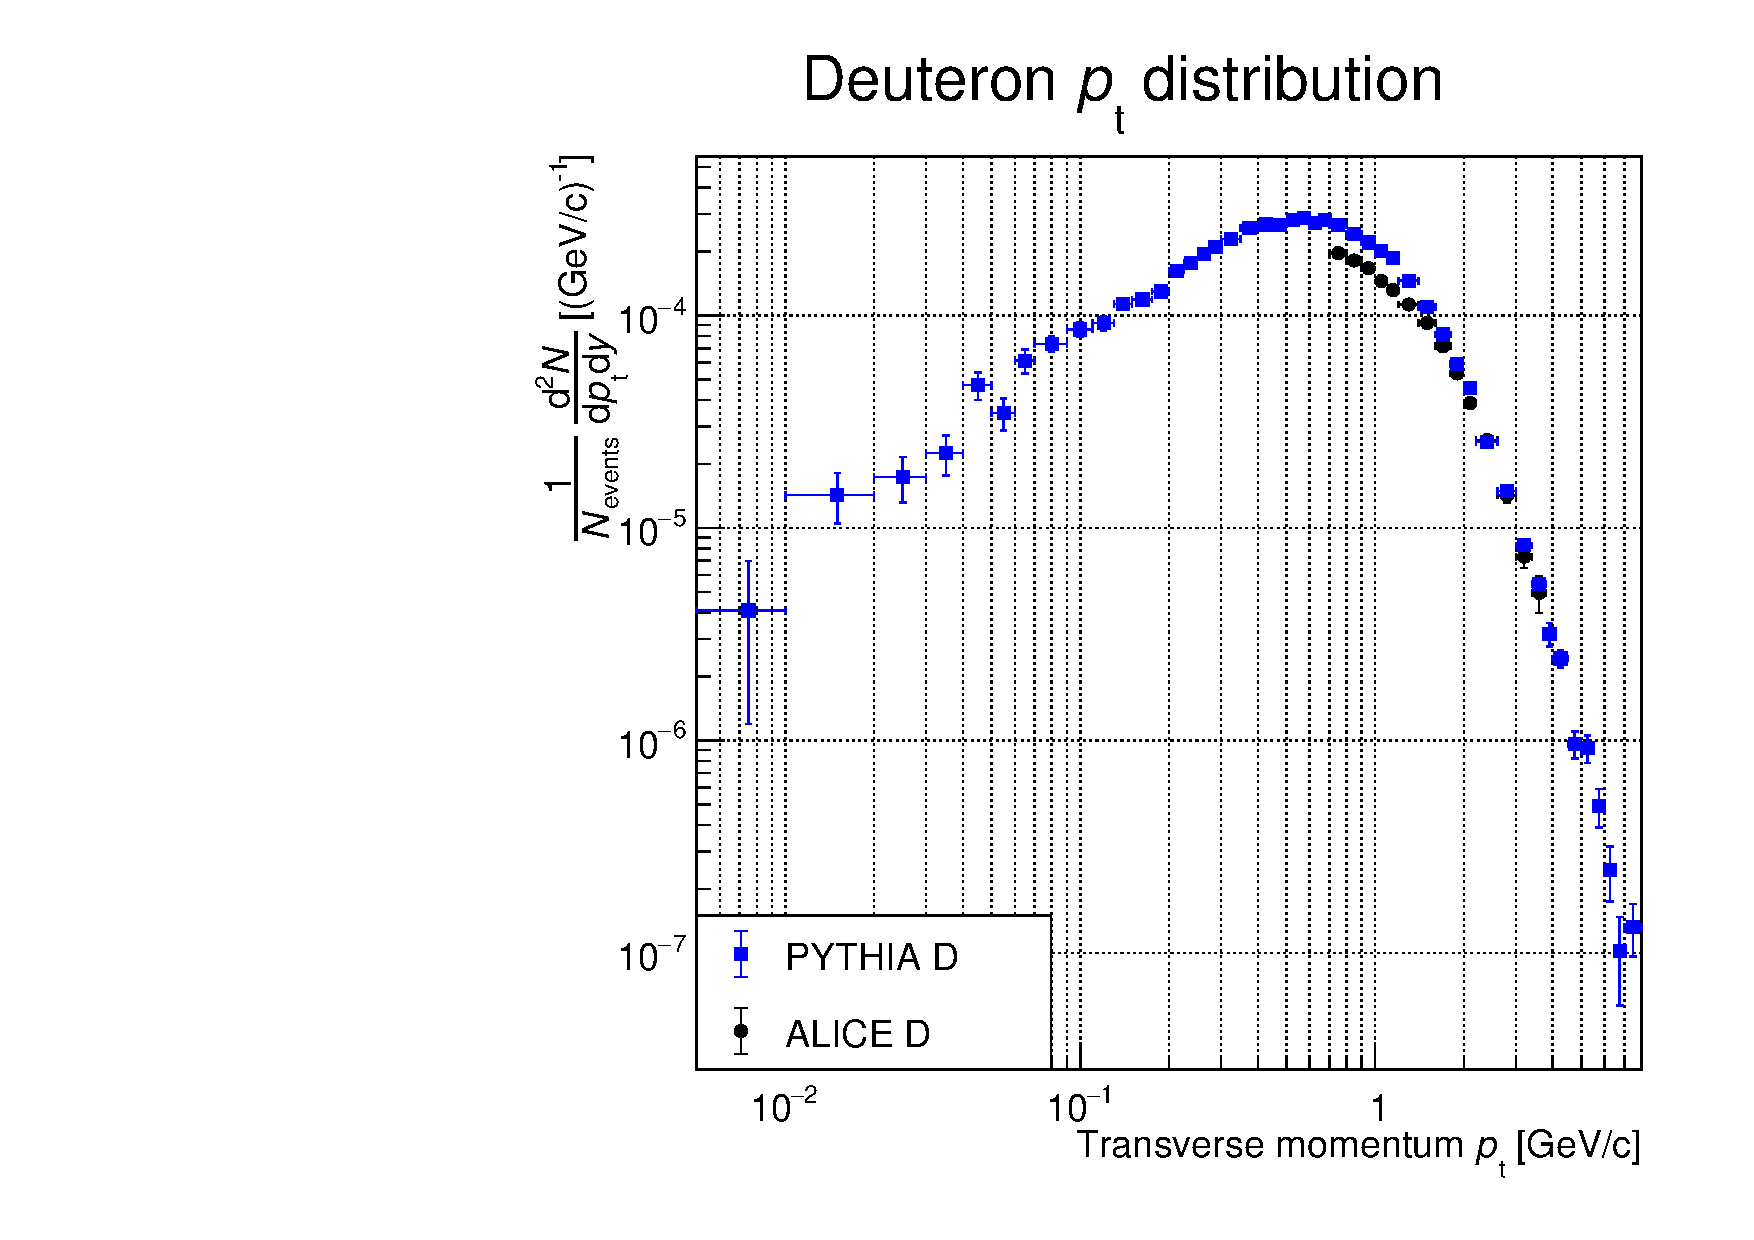
\includegraphics[width=\textwidth]{image/3-risultati/analyse/A/deuteron.pdf}
        \caption{}
        \label{fig:A_deuteron}
    \end{subfigure}
    %\hspace{1cm}
    \begin{subfigure}{.49\textwidth}
        \centering
        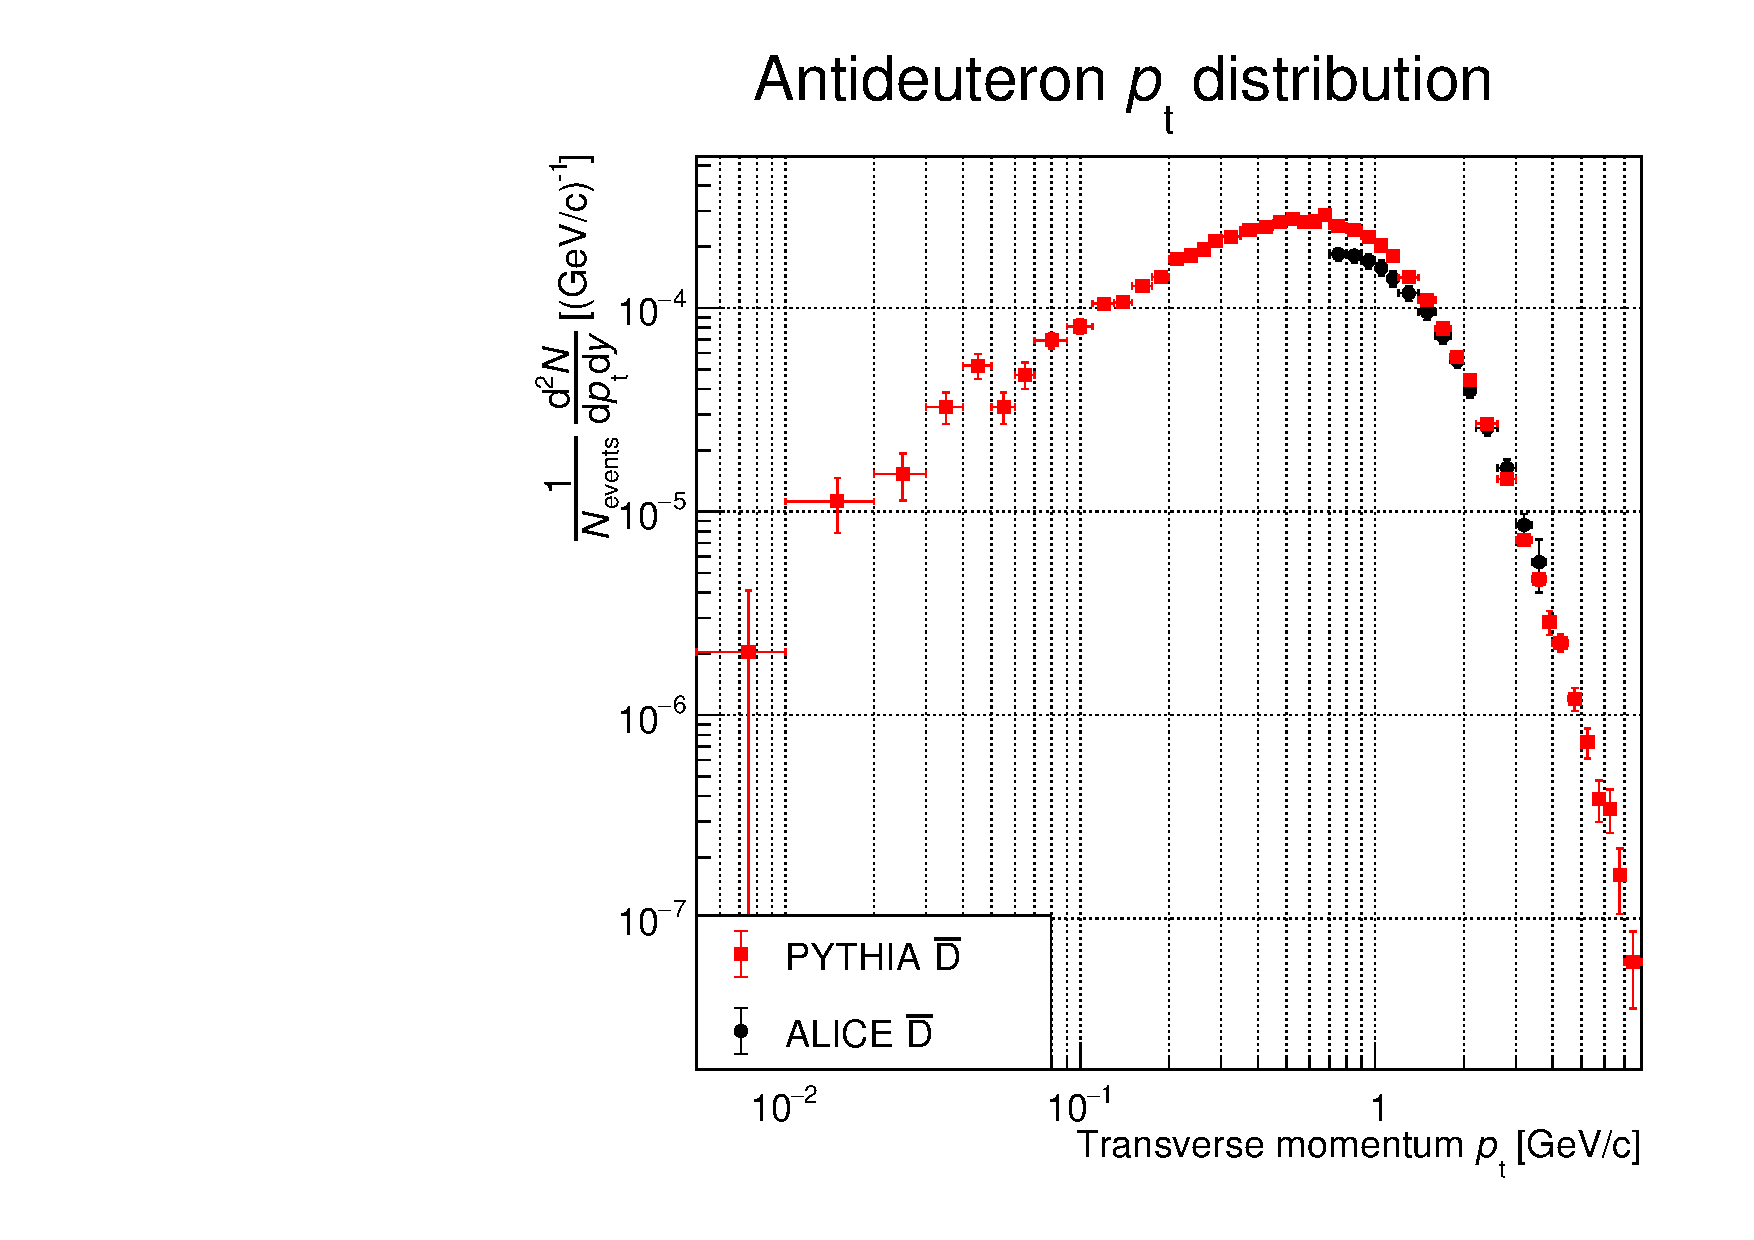
\includegraphics[width=\textwidth]{image/3-risultati/analyse/A/antideuteron.pdf}
        \caption{}
        \label{fig:A_antideuteron}
    \end{subfigure}
    \captionwithsource{Distribuzione dell'impulso trasverso di \emph{\rmfamily (a)} $D$ e \emph{\rmfamily (b)} di $\bar D$ in confronto con i dati di ALICE.}{\cite{ALICE:2020foi}}
    \label{fig:A_(anti)deuteron}
\end{figure}

In \autoref{fig:A_pp} osserviamo lo spettro di produzione della somma di protoni e antiprotoni nel caso in cui la produzione deuteronica sia attivata e non attivata, messo in confronto con i dati sperimentali.
Da questo grafico possiamo dedurre che la riproduzione di \pythiaa{} dello spettro dei protoni è fedele solamente nell'intorno di $p_t \sim 1$ GeV/$c$.
Gli andamenti degli spettri con produzione attivata e disattivata non presentano  particolari differenze, se non negli impulsi più alti, ma ciò è dovuto alle maggiori fluttuazioni dovute alla minore statistica.
Eseguendo un rapporto dei due istogrammi, visibile in \autoref{fig:A_ratio_pp_ON_OFF}, si ottiene che la media pesata del valore della frazione risulta essere $0.9988 \pm 0.0002$, inferiore a 1, compatibile con il valore atteso di 0.999.
Bisogna menzionare che le predizioni per la produzione di protoni da \pythiaa{} sono note per non descrivere fedelmente le misure sperimentali.
Questo è perché il tune di \pythiaa{} non è stato ottimizzato per riprodurre la produzione di nucleoni all'LHC, ma è comunque utilizzato come base per la maggior parte delle predizioni ed è stato utilizzato per la stima dei parametri per la sezione d'urto efficace, giustificando la scelta del \textit{tuning} per questo studio.
La produzione dei (anti)nuclei dipende essa stessa dallo spettro di produzione di protoni, che risulta interconnessa con tali parametri, ma la descrizione delle misure di protoni esula dallo scopo di questa tesi.

Se andiamo a confrontare invece lo spettro dei deuteroni e degli antideuteroni con i dati di ALICE \cite{ALICE:2020foi}, osserviamo in \autoref{fig:A_(anti)deuteron} che la produzione (anti)deuteronica è accurata solamente per gli impulsi più alti, nell'intorno di $p_t \sim 3$ GeV/$c$.
Infatti, eseguendo una divisione tra i dati di \pythia e di ALICE per i (anti)deuteroni, è possibile osservare che il rapporto si avvicina al valore unitario in quell'intorno, come si vede in \autoref{fig:A_division}.
In generale si osserva una sovrapproduzione sia per i deuteroni e sia per gli antideuteroni, con le medie pesate rispettivamente di $1.203 \pm 0.017$ e di $1.129 \pm 0.023$.
\begin{figure}[htb]
    \centering
    \begin{subfigure}{.49\textwidth}
    \centering
        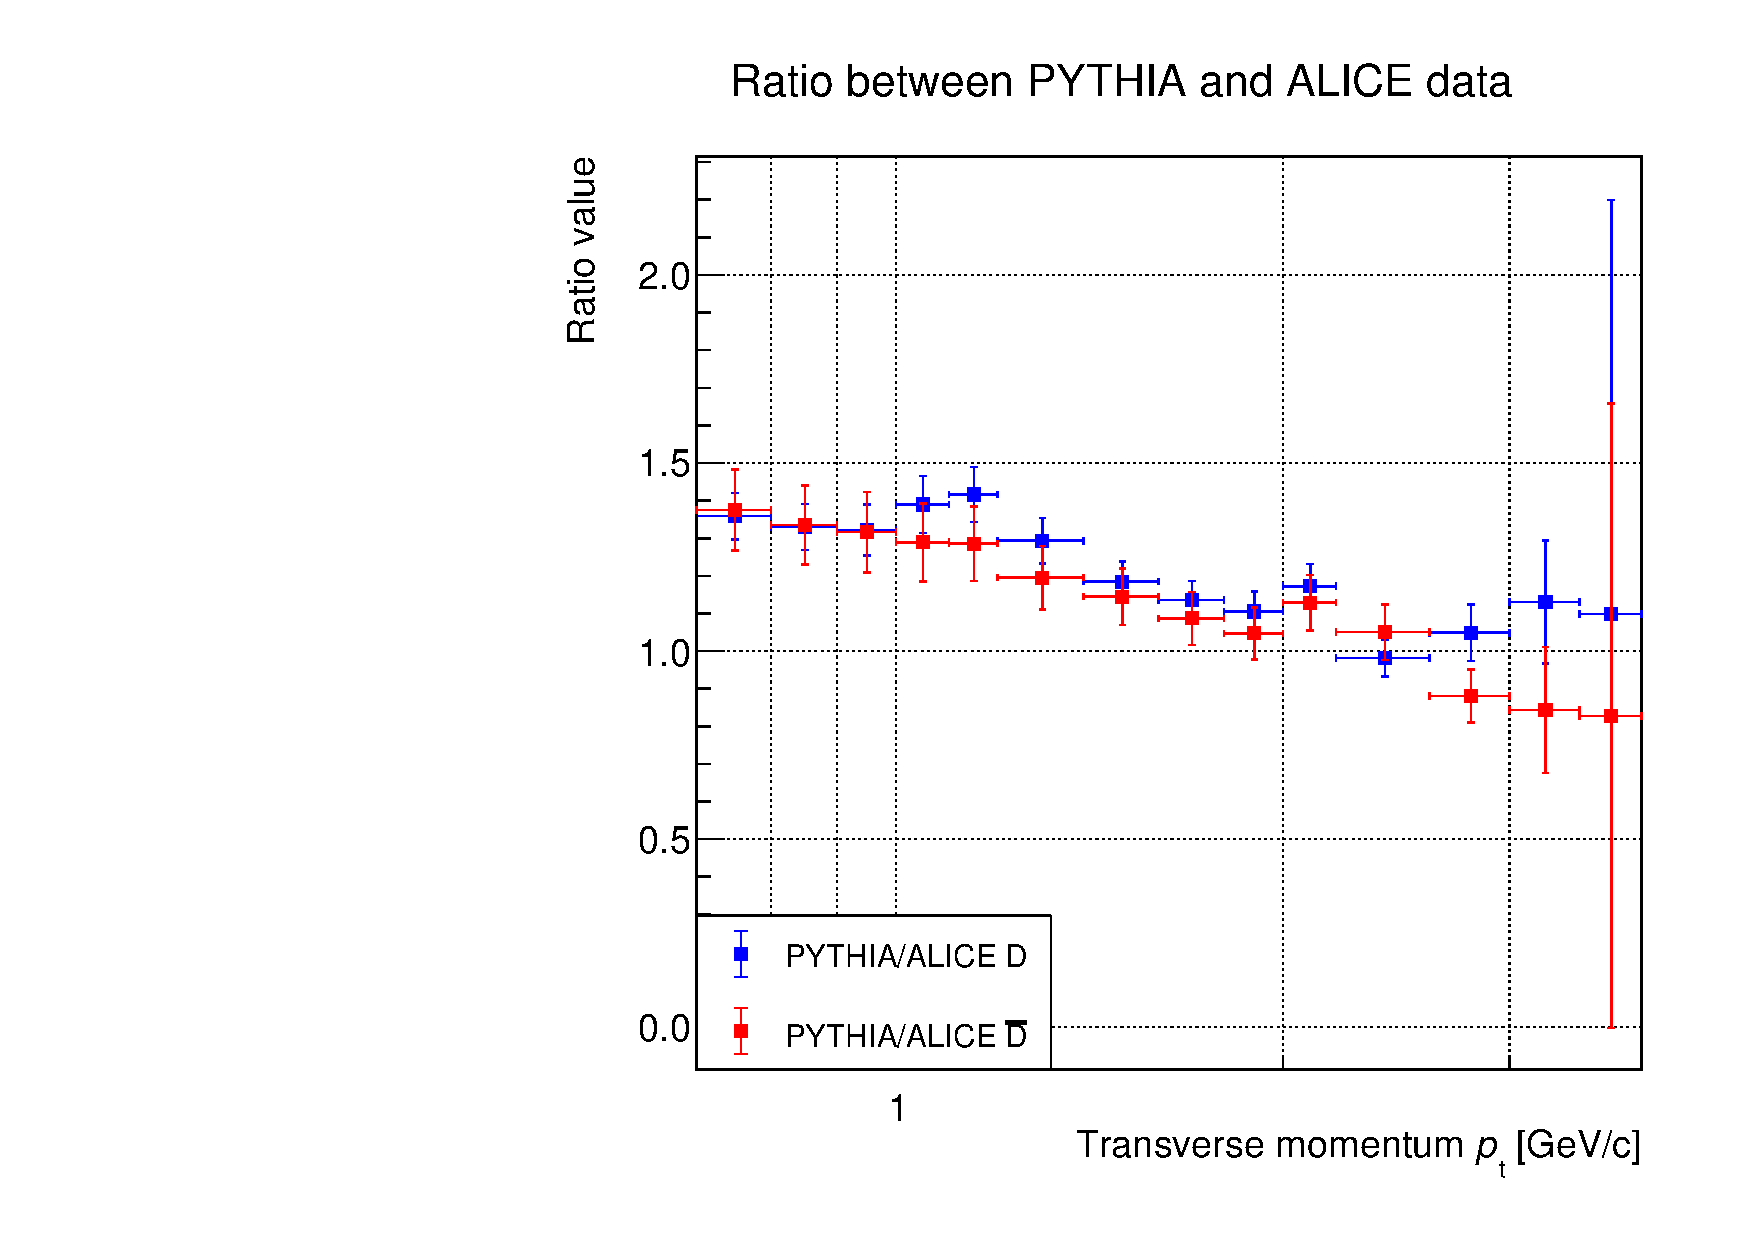
\includegraphics[width=\textwidth]{image/3-risultati/analyse/A/division.pdf}
        \caption{}
        \label{fig:A_division}
    \end{subfigure}
    %\hspace{1cm}
    \begin{subfigure}{.49\textwidth}
        \centering
        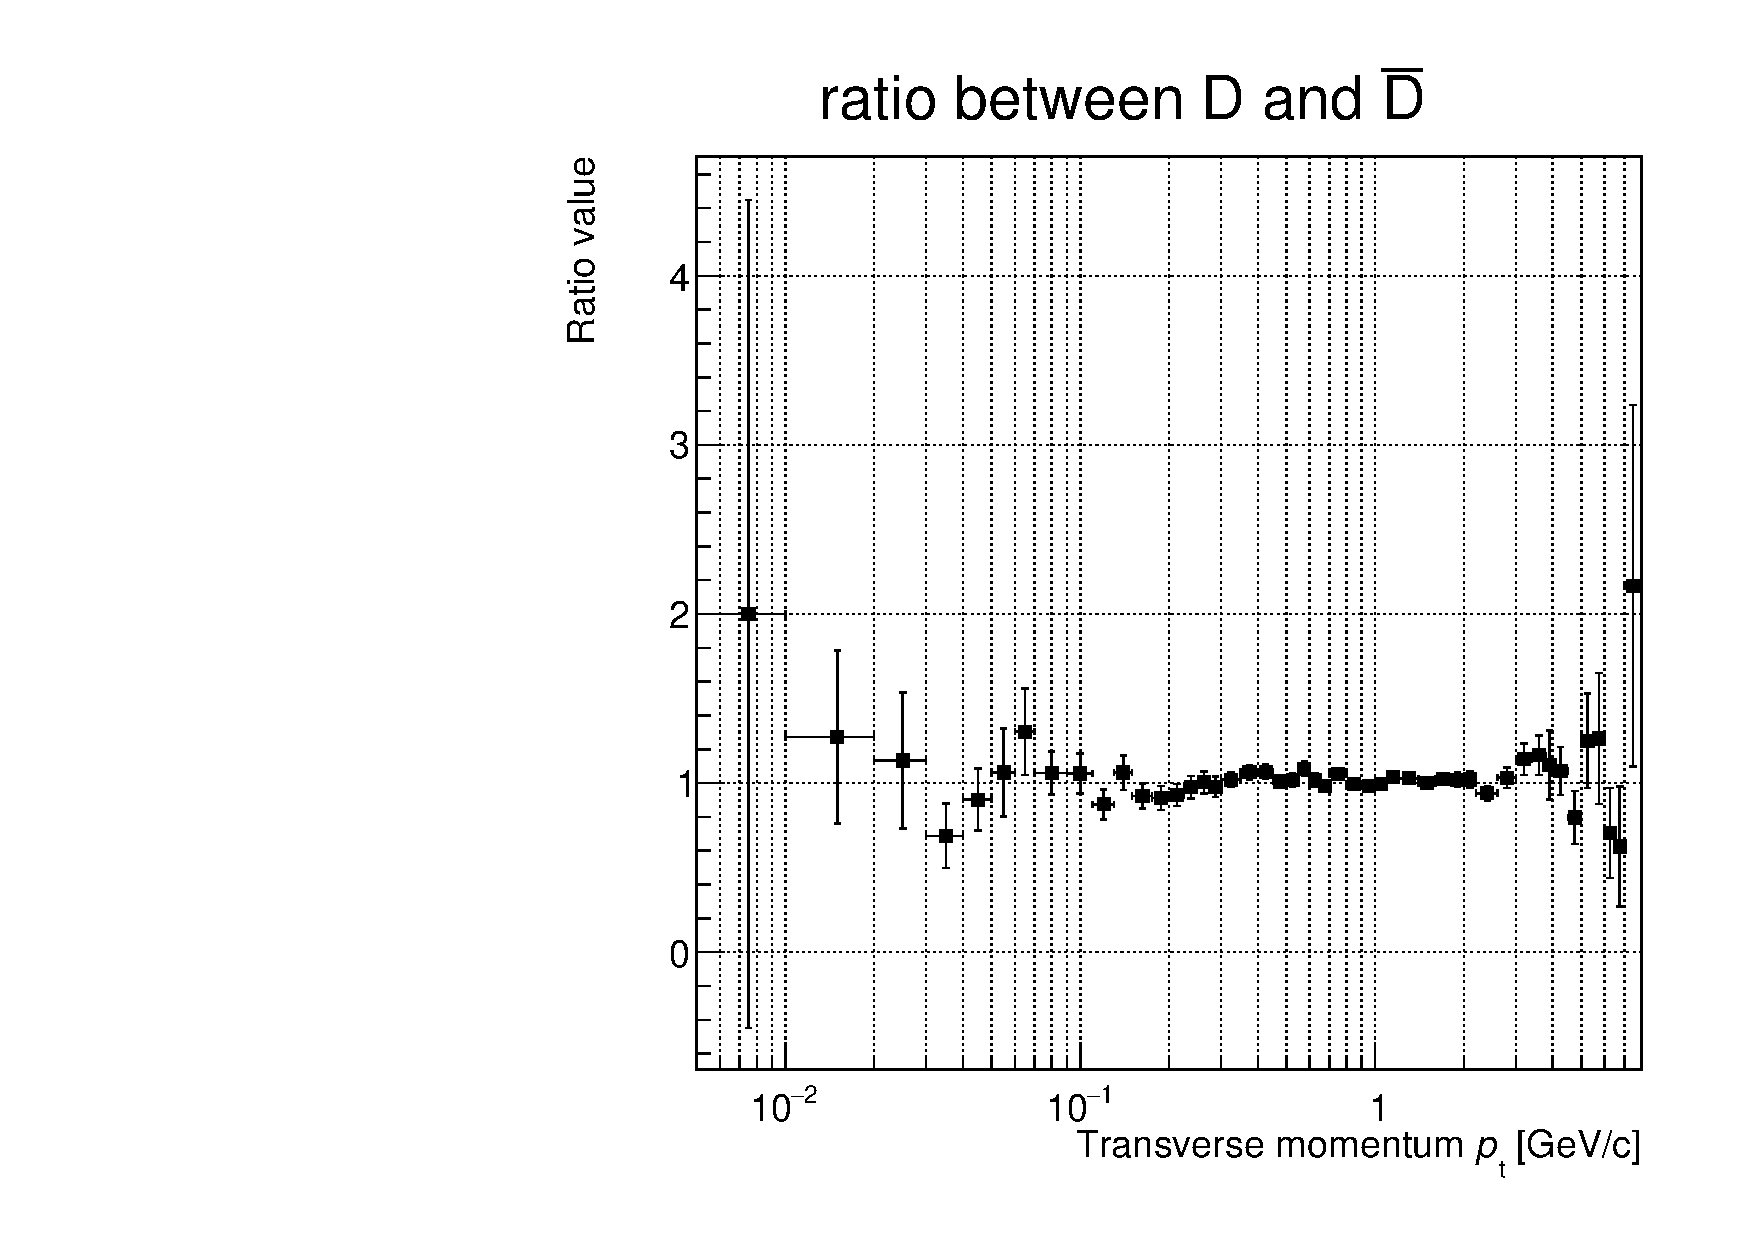
\includegraphics[width=\textwidth]{image/3-risultati/analyse/A/ratio_DD.pdf}
        \caption{}
        \label{fig:A_ratio_DD}
    \end{subfigure}
    \caption{\emph{\rmfamily (a)} Divisione tra la distribuzione dell'impulso trasverso di $D$ e $\bar D$ con i dati di ALICE. \emph{\rmfamily (b)} Rapporto delle distribuzione dell'impulso trasverso di $D$ con quello di $\bar D$.}
    \label{fig:A_ratio_DD_}
\end{figure}

Per verificare ulteriormente la correttezza delle predizioni si è fatto un ulteriore rapporto, riportato in \autoref{fig:A_ratio_DD}, tra lo spettro dei deuteroni e lo spettro degli antideuteroni.
La media pesata del rapporto risulta essere $1.013 \pm 0.008$, con una leggera sovrapproduzione di deuteroni.
%%%%%%%%%%%%%%%%%%%%%%%%%%%%%%%%%%%%%%%%%%
\section{I principali canali di produzione}\label{ch:channels}
Andando ad analizzare invece quali siano i canali che producono più deuteroni, si è andati \textit{in primis} a riempire gli istogrammi relativi alle particelle di partenza, ossia si è andato a vedere per ogni deuterone prodotto quali siano le loro particelle madri.
Per semplificare la nomenclatura, prendendo in considerazione la \autoref{tab:canali}, chiameremo i canali (1-4) "canali $pn$", i canali (5-6) "canali $pp$" e i canali (7-8) "canali $nn$".
Lo stesso vale per gli antideuteroni con canali $\bar p\bar n$, $\bar p\bar p$ e $\bar n\bar n$.
Da ciò abbiamo tre distribuzioni per i deuteroni e tre per gli antideuteroni, rispettivamente con i canali $pn$, $pp$, $nn$ e $\bar p\bar n$, $\bar p\bar p$, $\bar n\bar n$.
In \autoref{fig:A_ov_deut} e in \autoref{fig:A_ov_antideut} vengono riportate le distribuzioni di questi canali in sovrapposizione, mentre in \autoref{fig:A_ov_stack_deut} e in \autoref{fig:A_ov_stack_antideut} viene riportata la produzione relativa di (anti)deuteroni.  
Si può osservare che \pythiaa{} assegna a ognuno di questi canali uno stesso peso nella produzione sia deuteronica e sia antideuteronica, se non per un piccolo incremento per il canale $pn$ nei deuteroni e il canale $\bar p\bar n$ negli antideuteroni.\\

Successivamente si è andati ad analizzare la produzione relativa dei subcanali dei canali $pn$, $pp$ e $nn$ e delle relative antiparticelle, andando a vedere quali siano i loro principali contributi.
In \autoref{fig:A_deut_subchannels} e in \autoref{fig:A_antideut_subchannels} possiamo osservare tali contributi.
Si nota che il contributo più abbondante per tutti e sei i canali è quello in cui avviene la produzione di un (anti)deuterone e di un pione, mentre il contributo minore nella produzione è la cattura radiativa.
Invece la produzione di un deuterone e di due pioni è meno abbondante, perché essa richiede più energia ed è meno probabile che avvenga.

È curioso notare che in \autoref{fig:A_pn_stack_deut} e in \autoref{fig:A_pn_stack_antideut} il processo $pn\to \pi^+\pi^- D$ ($ \bar p \bar n\to \pi^+\pi^- \bar D$) pare più abbondante del processo $pn\to \pi^0\pi^0D$ ($ \bar p \bar n\to \pi^0\pi^0 \bar D$).
Questo può essere spiegato con l'invarianza di isospin, per cui si ha che (\cite{Dal_2015})
\begin{equation}
    \sigma_{pn\to\pi^+\pi^-D} = 2\sigma_{pn\to\pi^0\pi^0D} + \dfrac12\sigma_{pp\to\pi^+\pi^0D}
\end{equation}
con $\sigma_\text{processo}$ la sezione d'urto del processo associato.
\begin{figure}[htbp]
    \centering
    \begin{subfigure}{.49\textwidth}
    \centering
        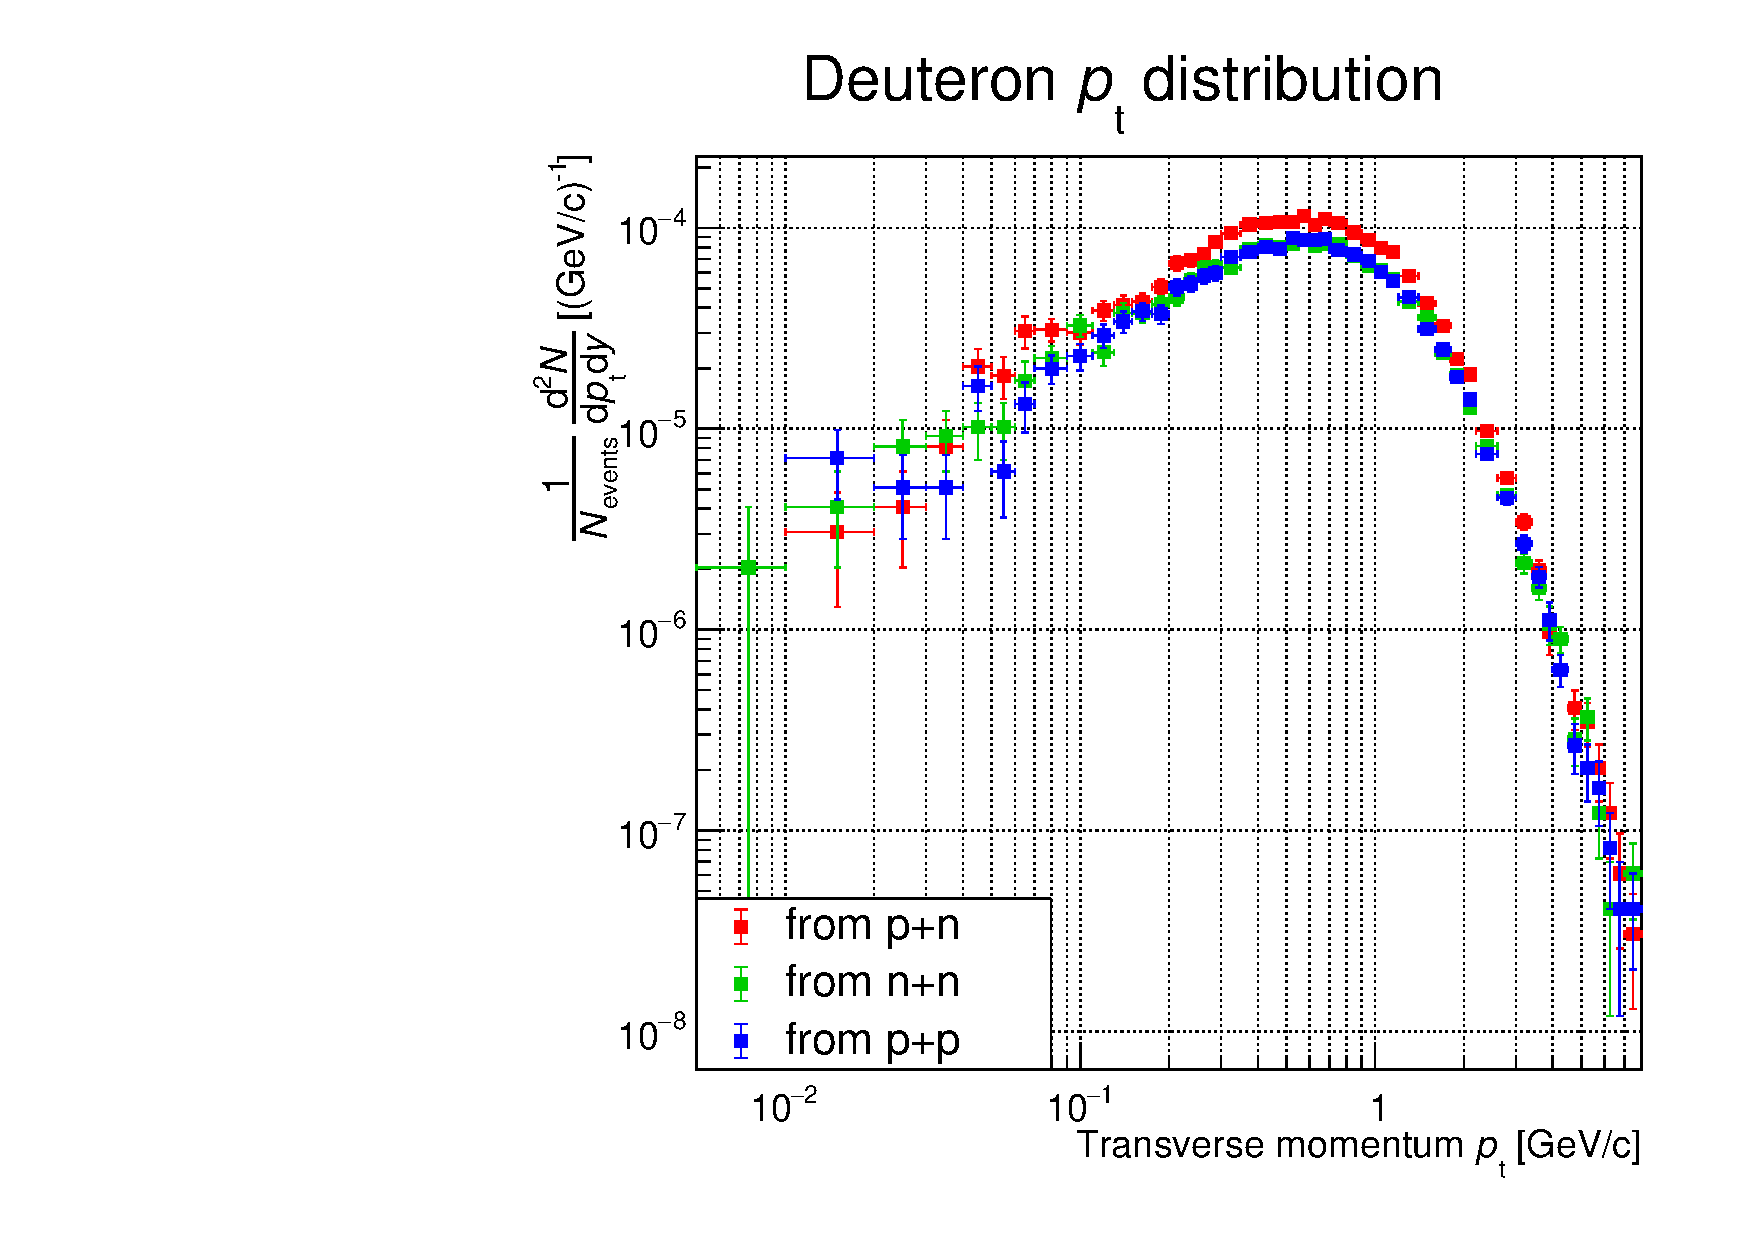
\includegraphics[width=\textwidth]{image/3-risultati/deuteron_analyse/A/ov_log.pdf}
        \caption{}
        \label{fig:A_ov_deut}
    \end{subfigure}
    %\hspace{1cm}
    \begin{subfigure}{.49\textwidth}
        \centering
        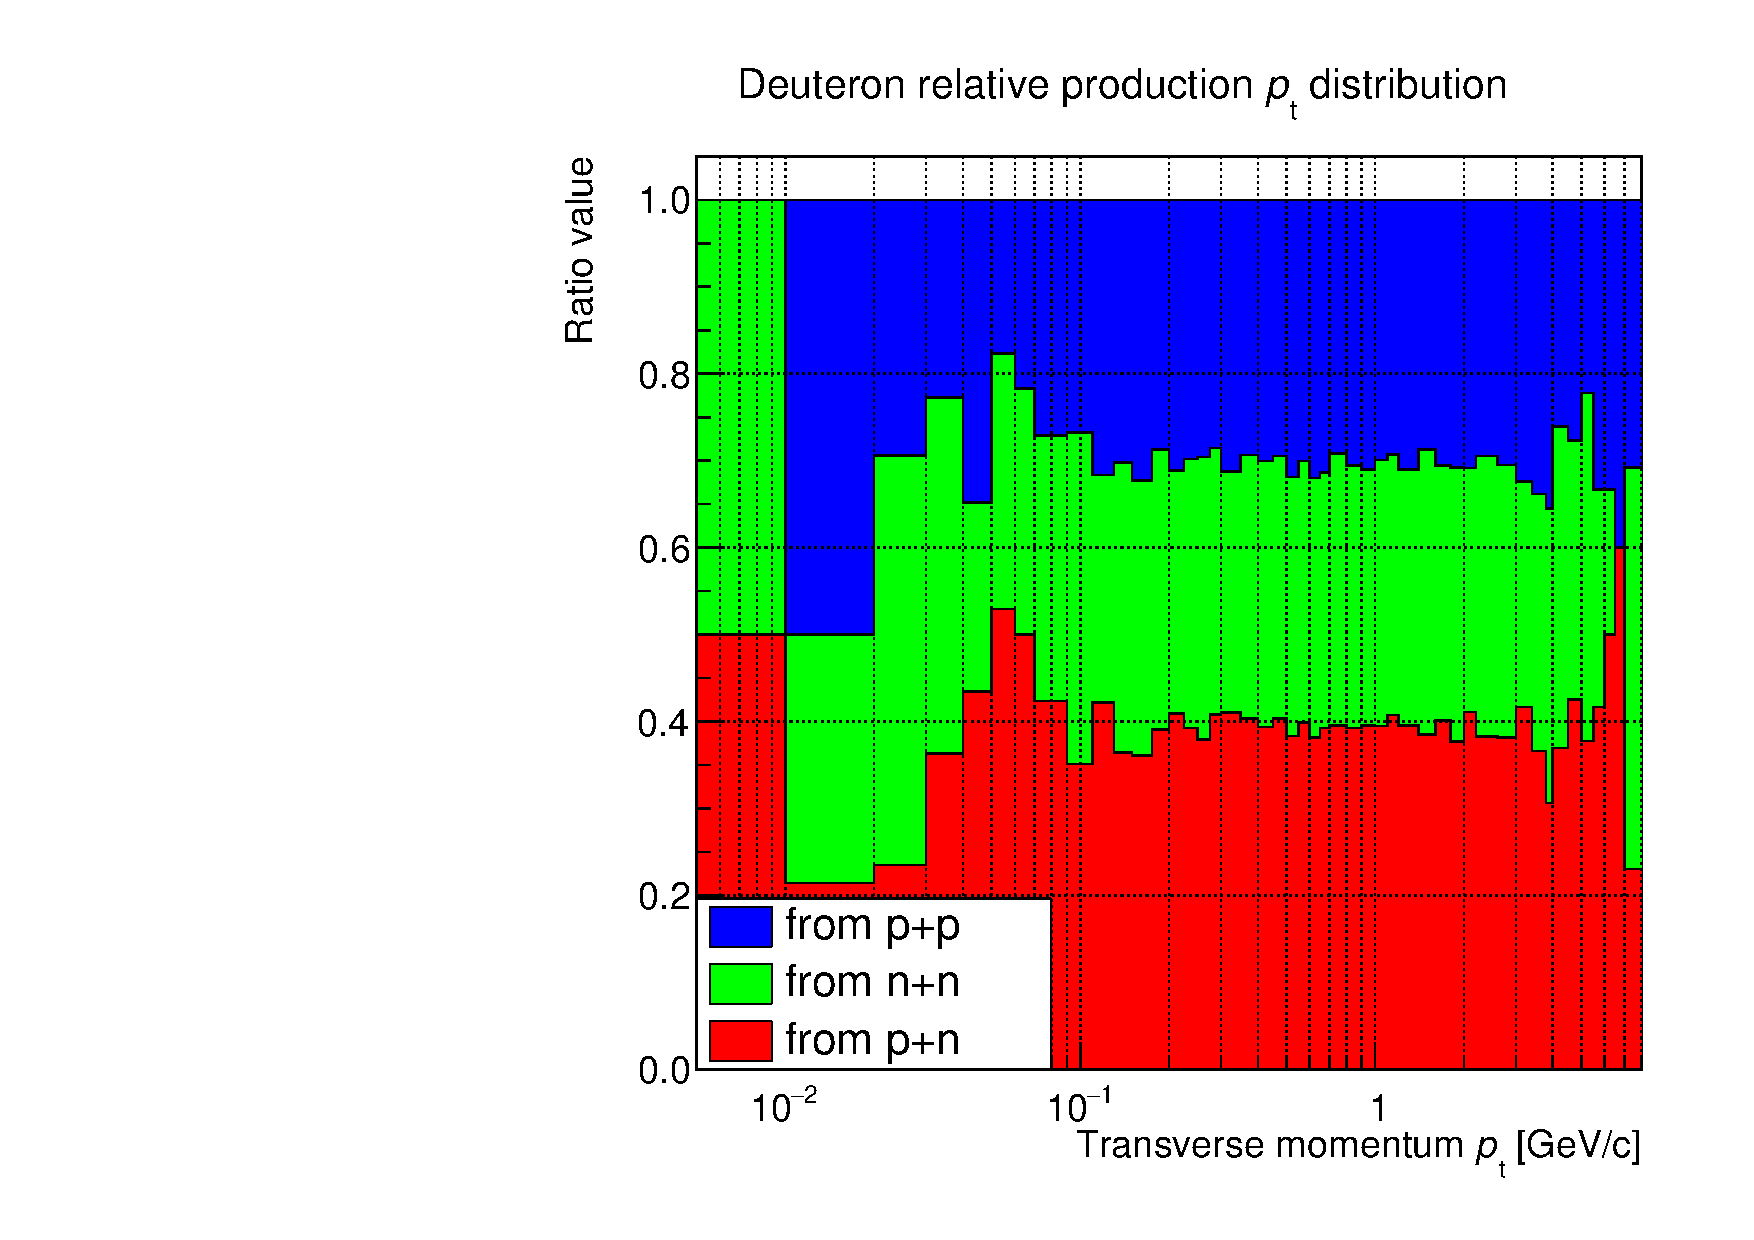
\includegraphics[width=\textwidth]{image/3-risultati/deuteron_analyse/A/ov_stack.pdf}
        \caption{}
        \label{fig:A_ov_stack_deut}
    \end{subfigure}
    \begin{subfigure}{.49\textwidth}
    \centering
        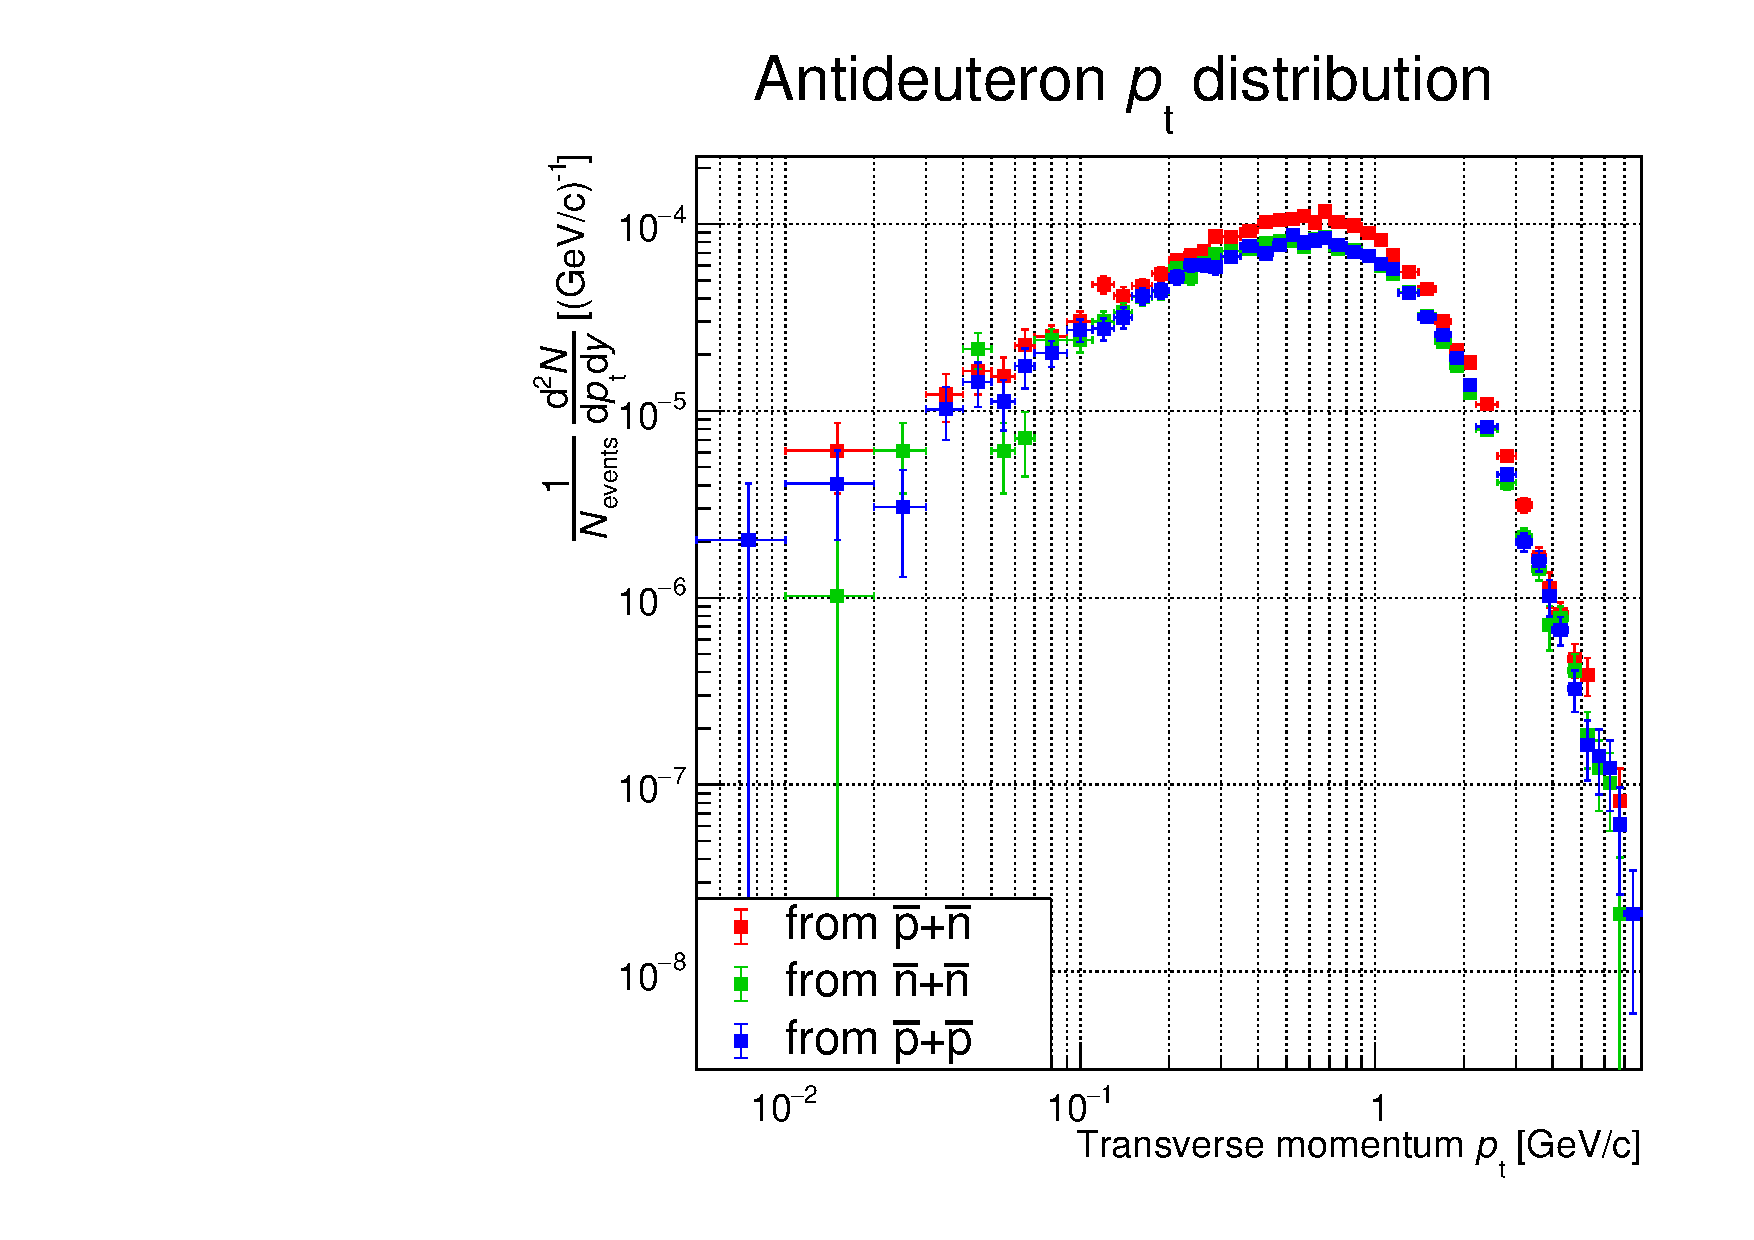
\includegraphics[width=\textwidth]{image/3-risultati/antideuteron_analyse/A/ov_log.pdf}
        \caption{}
        \label{fig:A_ov_antideut}
    \end{subfigure}
    %\hspace{1cm}
    \begin{subfigure}{.49\textwidth}
        \centering
        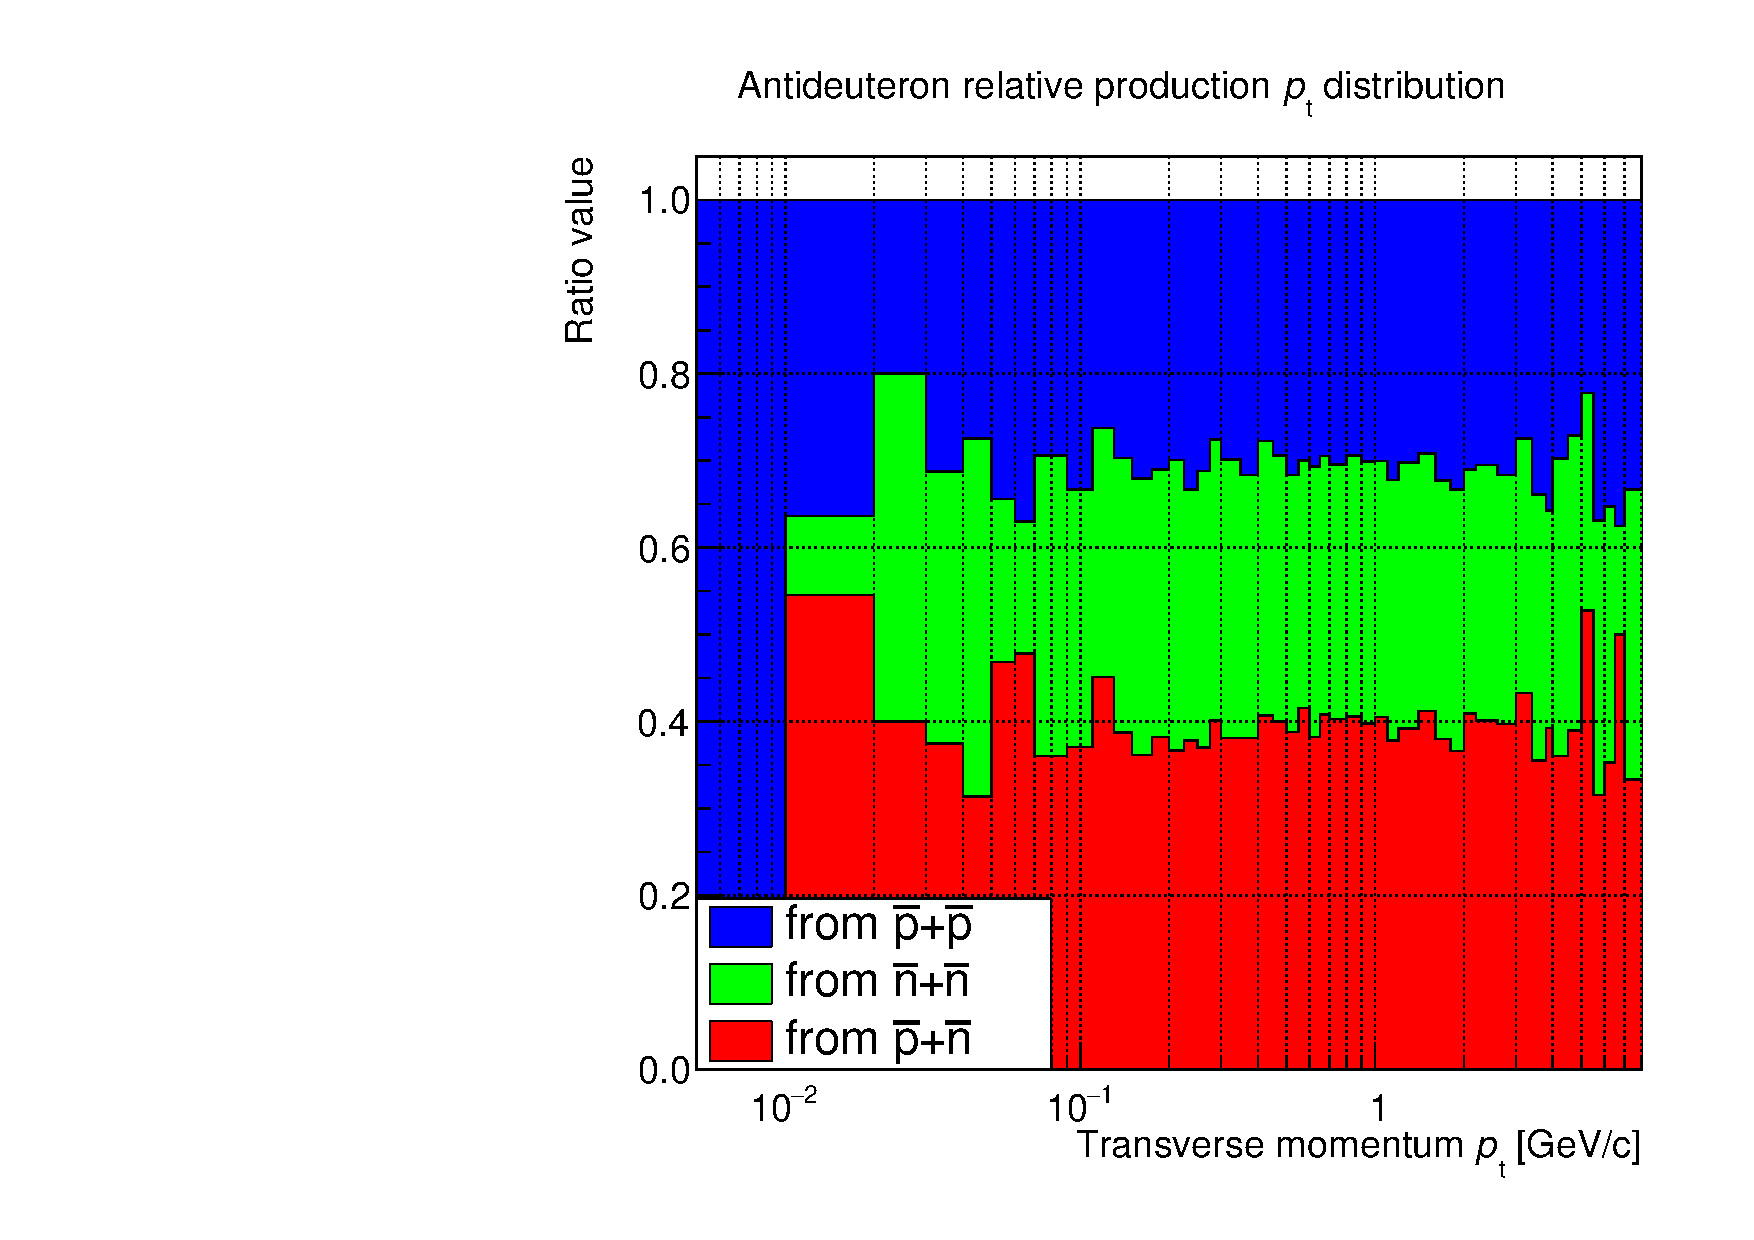
\includegraphics[width=\textwidth]{image/3-risultati/antideuteron_analyse/A/ov_stack.pdf}
        \caption{}
        \label{fig:A_ov_stack_antideut}
    \end{subfigure}
    \caption{\emph{\rmfamily (a)} Distribuzioni dell'impulso trasverso di $D$ dei canali $pn$, $pp$ e $nn$ e \emph{\rmfamily (b)} la produzione relativa nei vari canali di $D$. \emph{\rmfamily (c)} Distribuzioni dell'impulso trasverso di $\bar D$ dei canali $\bar p\bar n$, $\bar p\bar p$ e $\bar n\bar n$ e \emph{\rmfamily (d)} la produzione relativa nei vari canali di $\bar D$.}
    \label{fig:A_ov}
\end{figure}
\begin{figure}[htbp]
    \centering
    \begin{subfigure}{.49\textwidth}
    \centering
        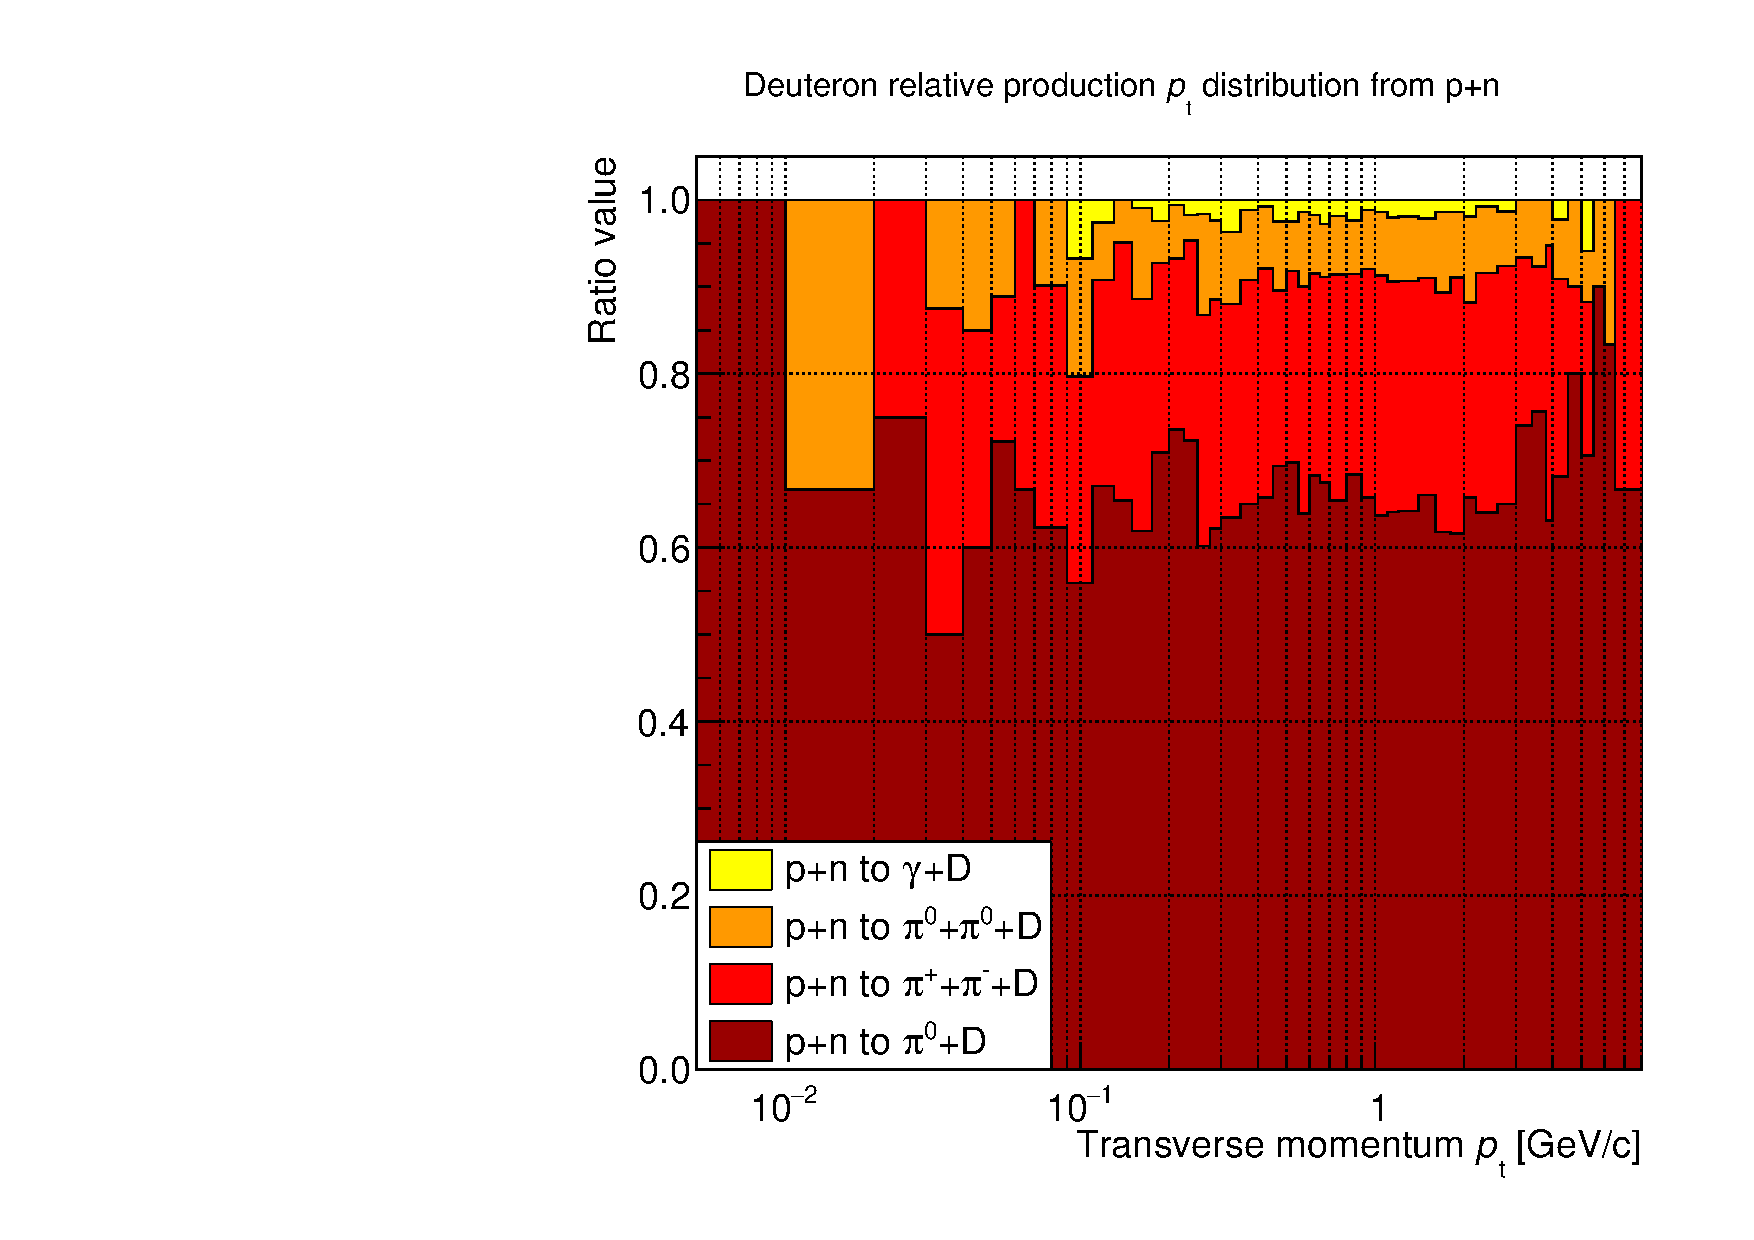
\includegraphics[width=\textwidth]{image/3-risultati/deuteron_analyse/A/p_n_stack.pdf}
        \caption{}
        \label{fig:A_pn_stack_deut}
    \end{subfigure}
    %\hspace{1cm}
    \begin{subfigure}{.49\textwidth}
        \centering
        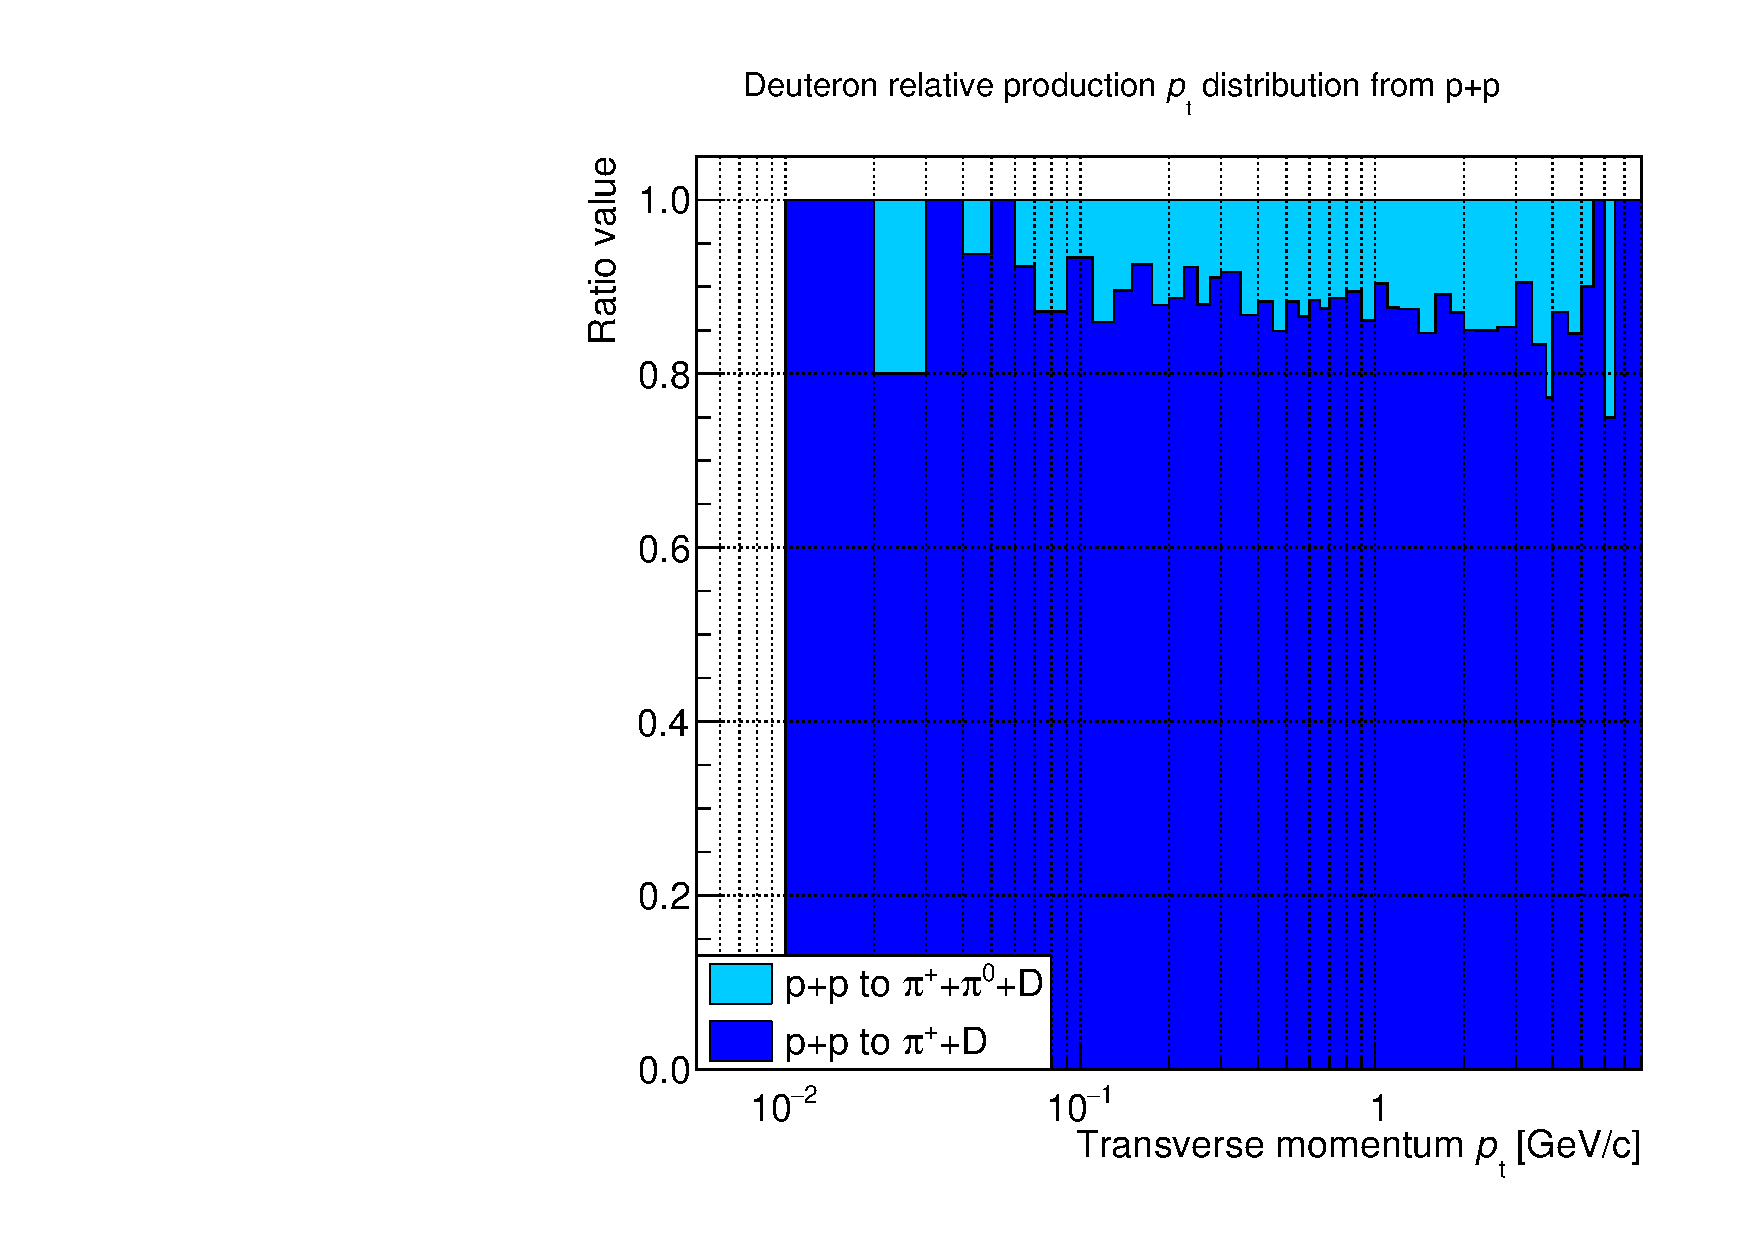
\includegraphics[width=\textwidth]{image/3-risultati/deuteron_analyse/A/p_p_stack.pdf}
        \caption{}
        \label{fig:A_pp_stack_deut}
    \end{subfigure}
    \begin{subfigure}{.49\textwidth}
    \centering
        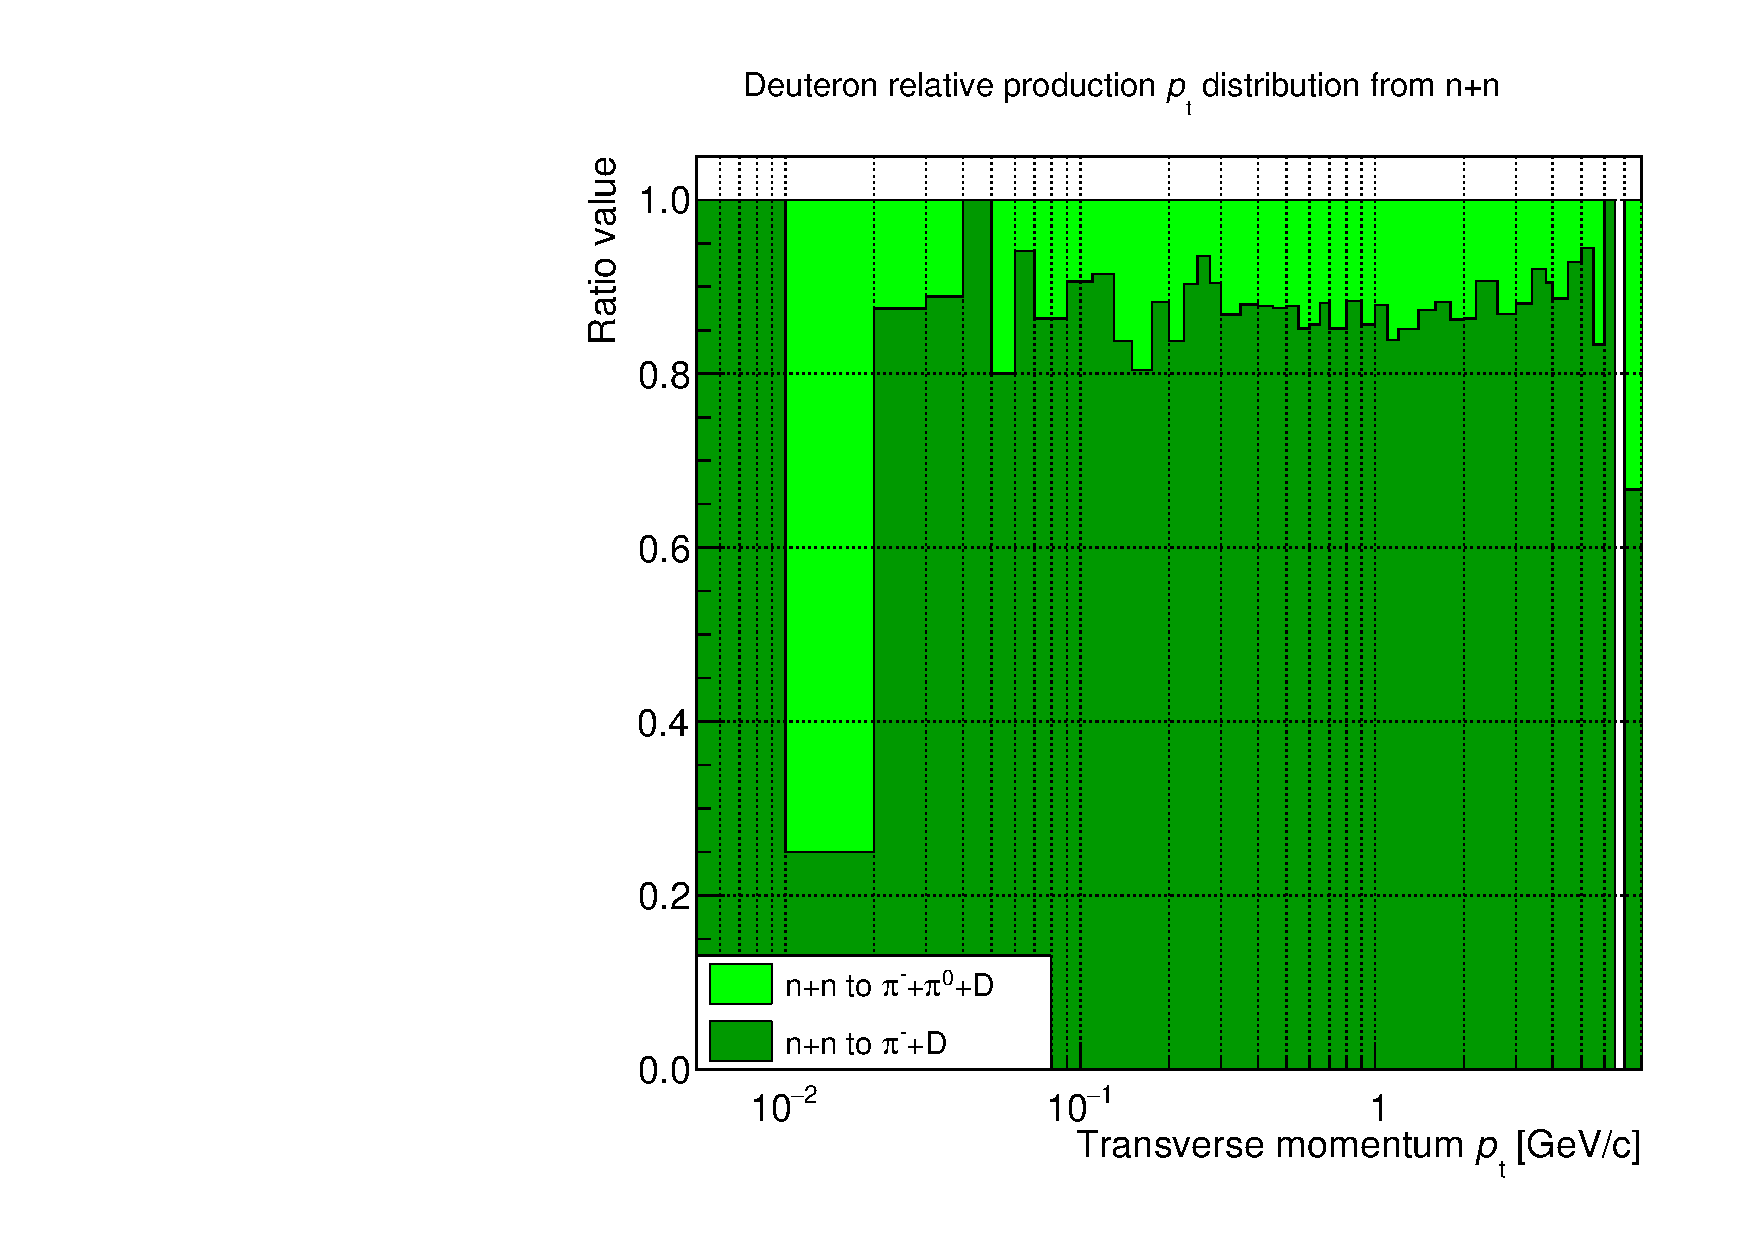
\includegraphics[width=\textwidth]{image/3-risultati/deuteron_analyse/A/n_n_stack.pdf}
        \caption{}
        \label{fig:A_nn_stack_deut}
    \end{subfigure}
    \caption{Produzione relativa di $D$ dei canali \emph{\rmfamily (a)} $pn$, \emph{\rmfamily (b)} $pp$ e \emph{\rmfamily (c)} $nn$.}
    \label{fig:A_deut_subchannels}
\end{figure}
\begin{figure}[htbp]
    \centering
    \begin{subfigure}{.49\textwidth}
    \centering
        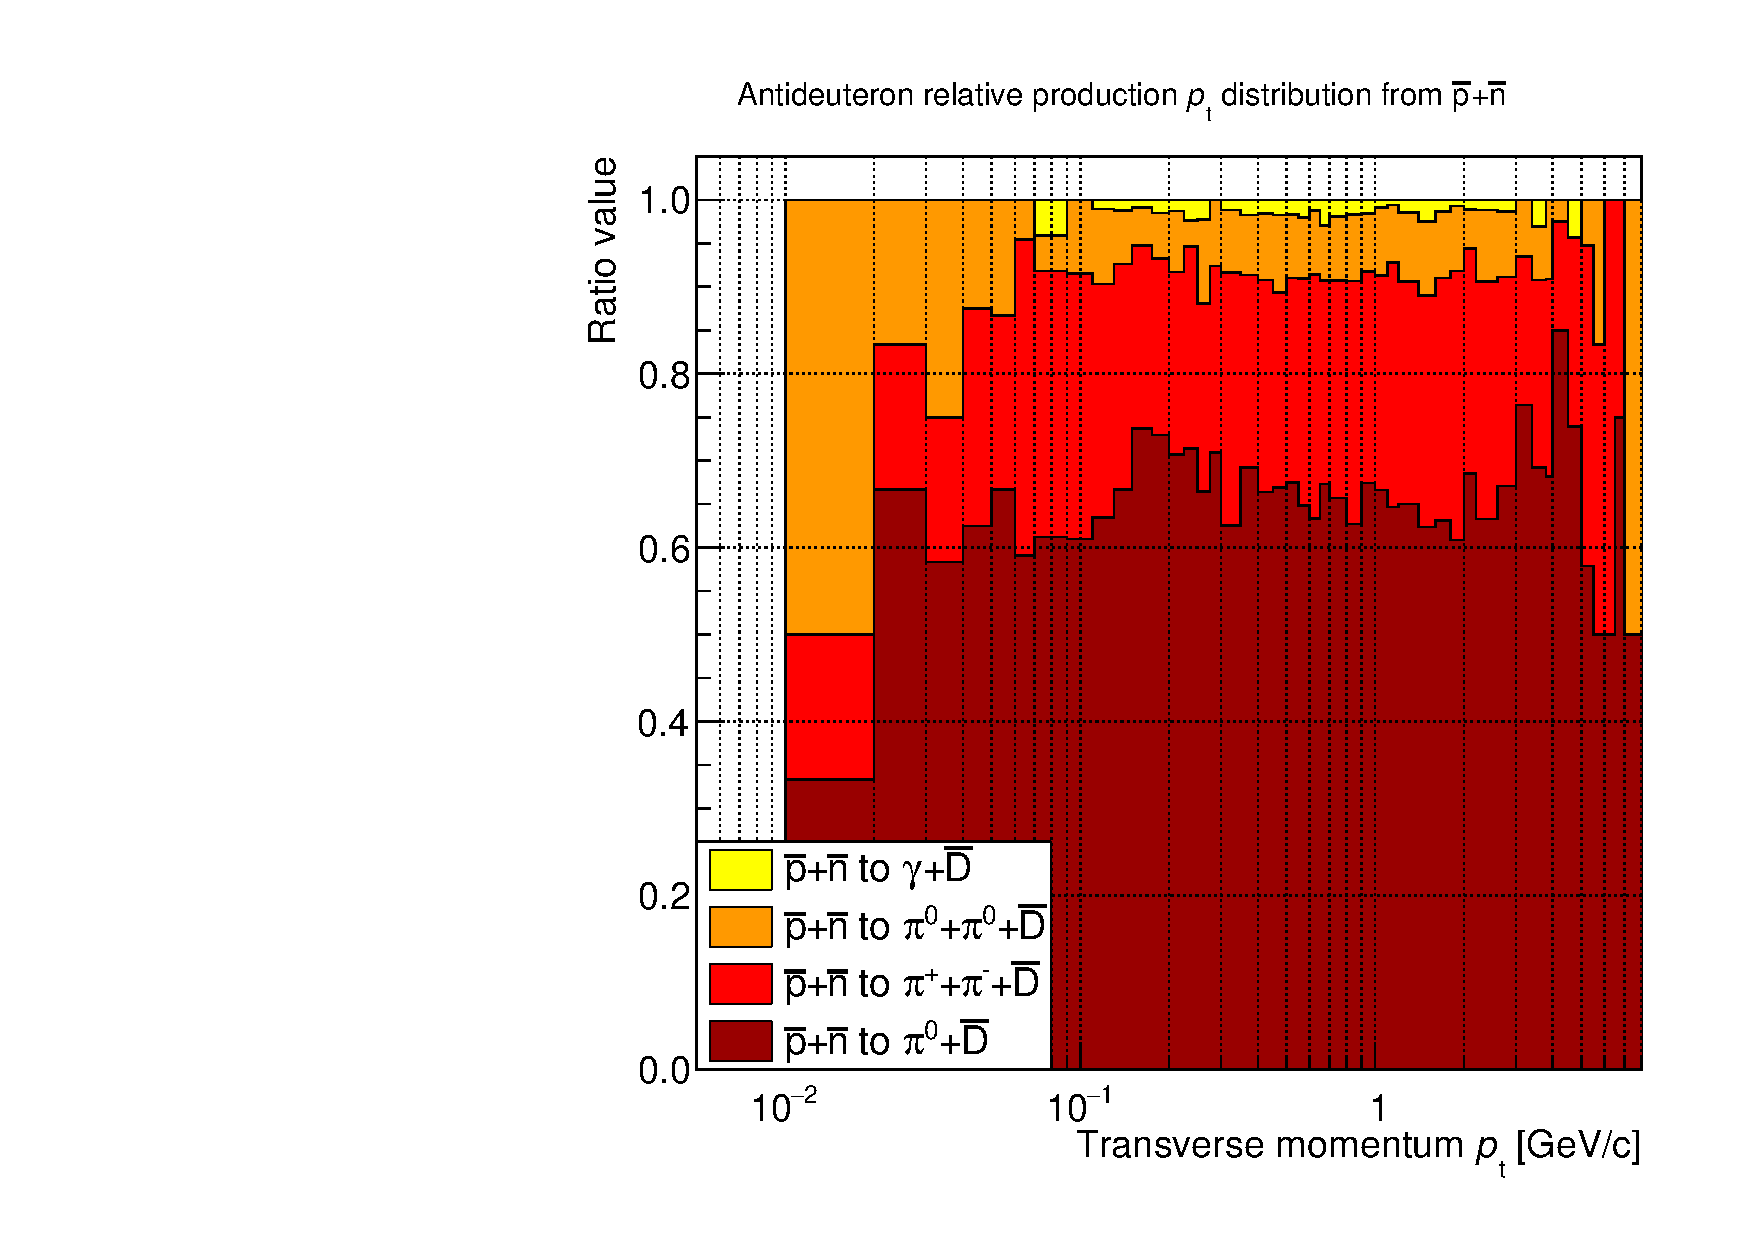
\includegraphics[width=\textwidth]{image/3-risultati/antideuteron_analyse/A/p_n_stack.pdf}
        \caption{}
        \label{fig:A_pn_stack_antideut}
    \end{subfigure}
    %\hspace{1cm}
    \begin{subfigure}{.49\textwidth}
        \centering
        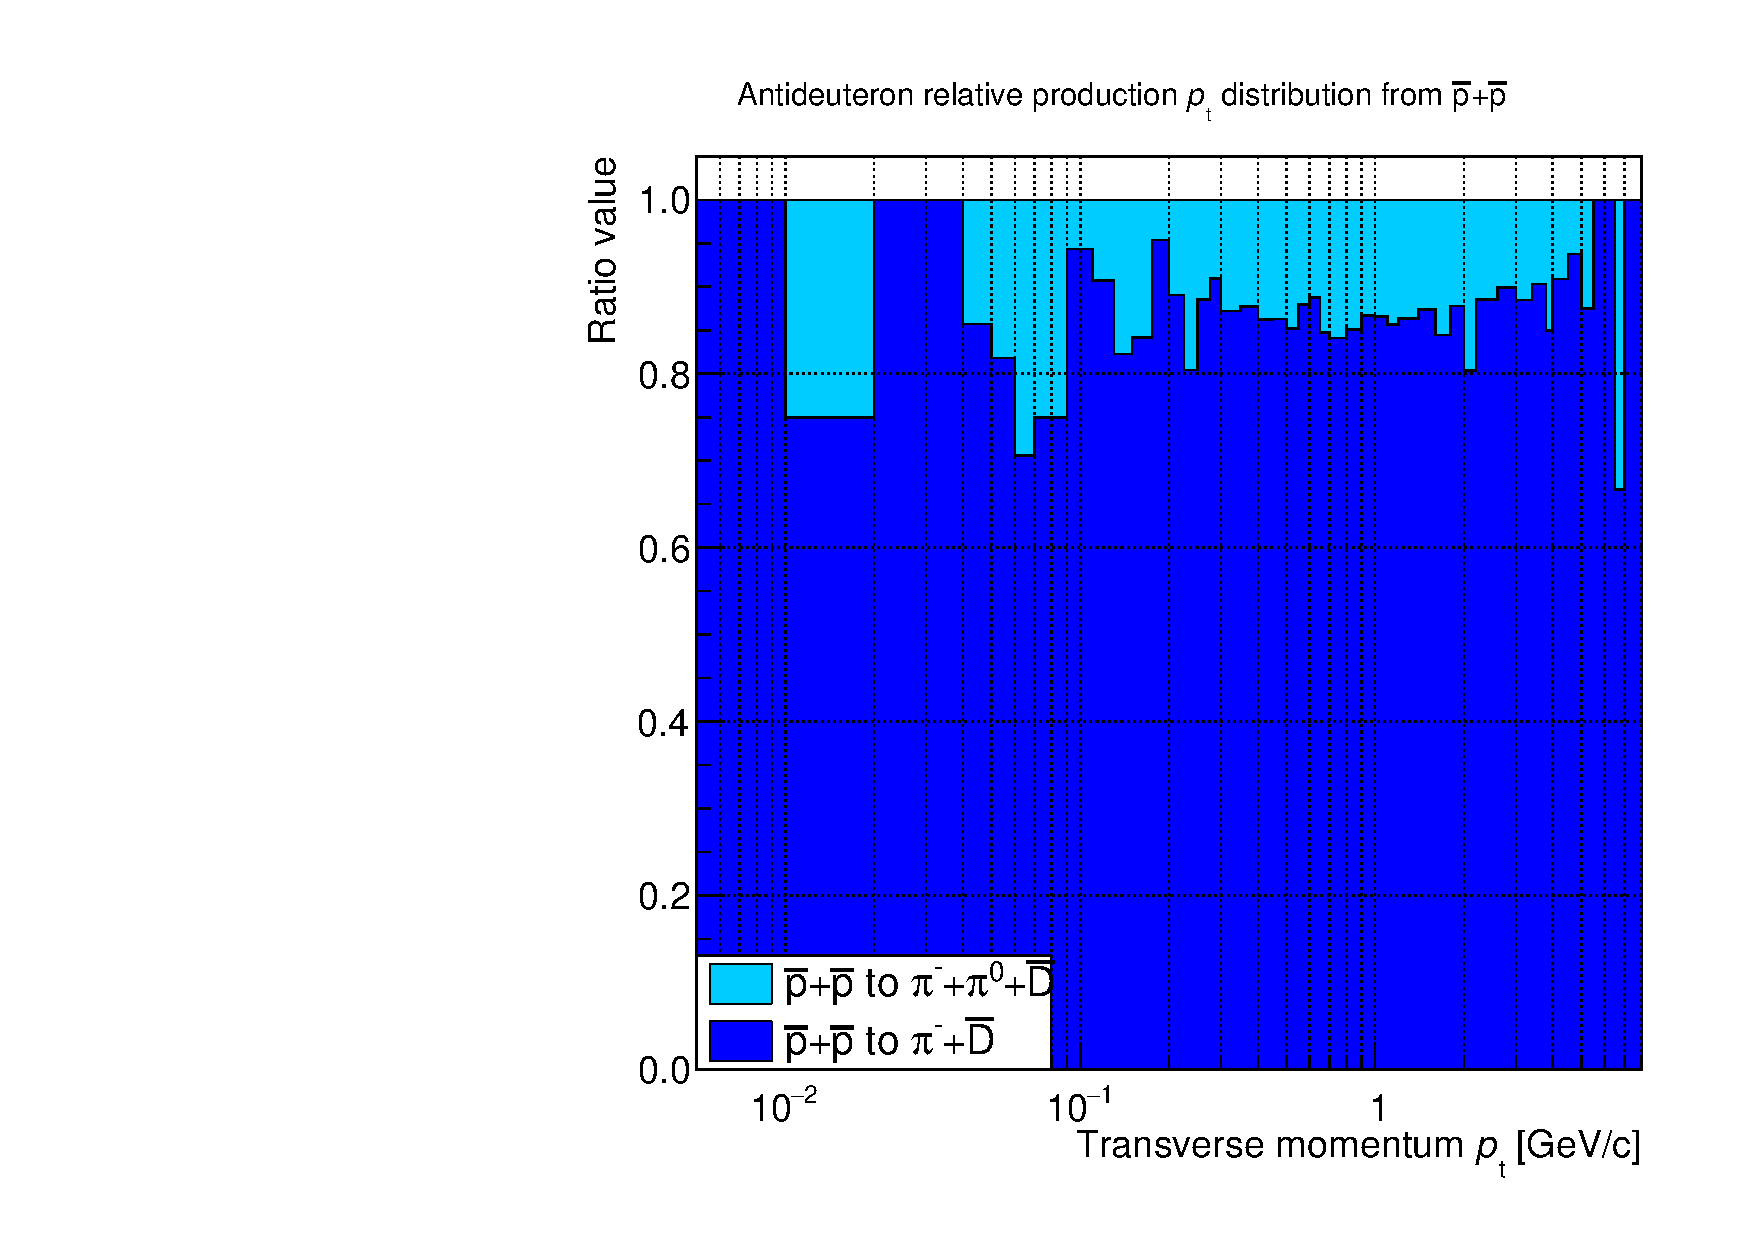
\includegraphics[width=\textwidth]{image/3-risultati/antideuteron_analyse/A/p_p_stack.pdf}
        \caption{}
        \label{fig:A_pp_stack_antideut}
    \end{subfigure}
    \begin{subfigure}{.49\textwidth}
    \centering
        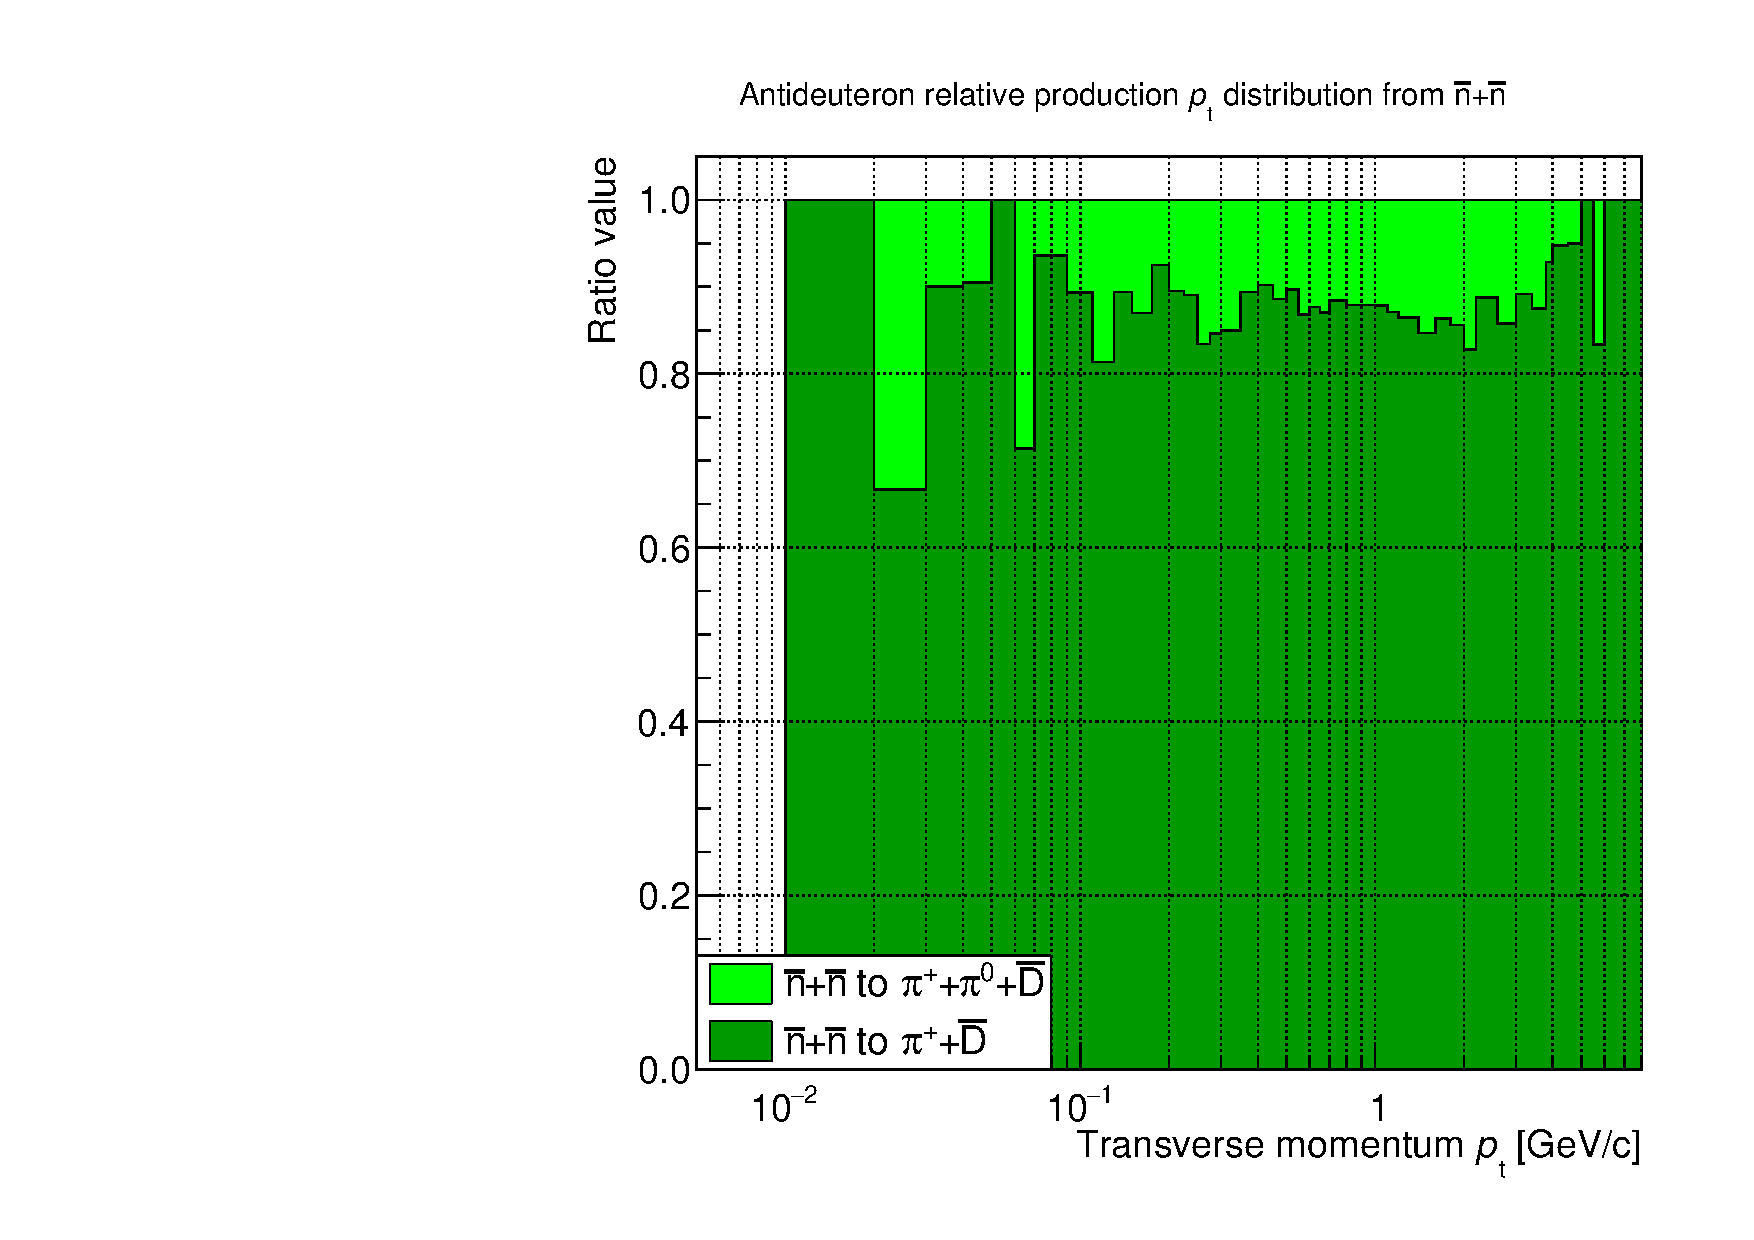
\includegraphics[width=\textwidth]{image/3-risultati/antideuteron_analyse/A/n_n_stack.pdf}
        \caption{}
        \label{fig:A_nn_stack_antideut}
    \end{subfigure}
    \caption{Produzione relativa di $\bar D$ dei canali \emph{\rmfamily (a)} $\bar p\bar n$, \emph{\rmfamily (b)} $\bar p\bar p$ e \emph{\rmfamily (c)} $\bar n\bar n$.}
    \label{fig:A_antideut_subchannels}
\end{figure}
%%%%%%%%%%%%%%%%%%%%%%%%%%%%%%%%%%%%%%%%%%%%%%%%%%%%
\section{Confronto del modello di coalescenza e di PYTHIA}
Sebbene non nella sua configurazione predefinita, \pythiaa{} ammette anche la produzione deuteronica tramite il modello di coalescenza.
Per far ciò si è andati a ridurre l'insieme di tutti i possibili canali di produzione al singolo canale della cattura radiativa (l'unico rilevante per la coalescenza), assegnando ad essa il modello di coalescenza con il parametro $p_0 = 195$ MeV.
La scelta di questo valore è giustificata da una semplice valutazione della \autoref{tab:valori_p0_1sigma0}: andando ad osservare la colonna $p_0$ si può dedurre che esso raggiunge stabilmente questo valore già a 7 TeV.
Dopodiché, oltre a questo, si è andati a imporre le condizioni già riportate nella \autoref{ch:settings} e si è effettuata la simulazione di Monte Carlo.\\

Andando a osservare lo spettro di produzione di $p+\bar p$ (visibile in \autoref{fig:E_pp}), non si nota una particolare differenza col modello predefinito, come deve essere, dal momento in cui il numero di (anti)deuteroni prodotti dovrebbe essere relativamente piccolo rispetto a quello dei protoni sia per il modello di \pythiaa{} sia per il modello di coalescenza.
\begin{figure}[htb]
    \centering
    \begin{subfigure}{.49\textwidth}
    \centering
        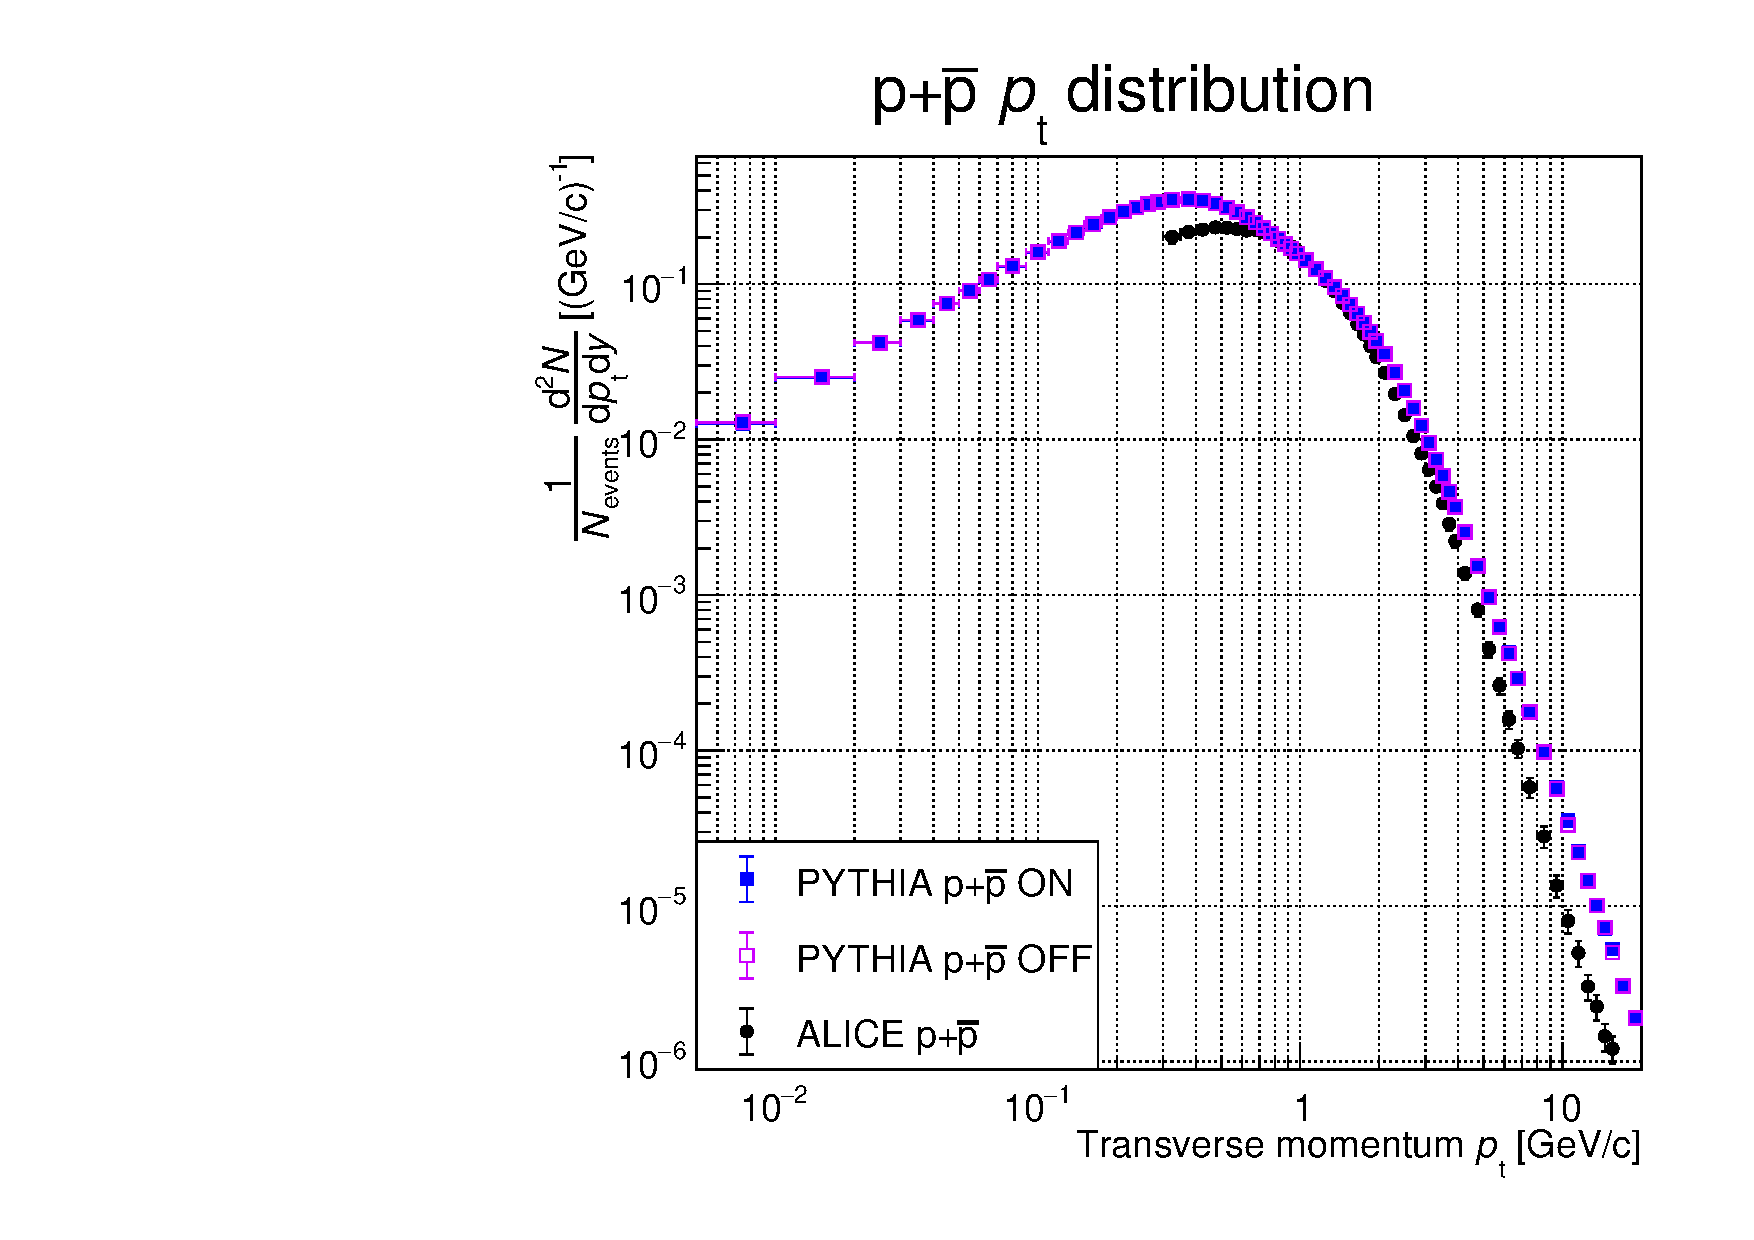
\includegraphics[width=\textwidth]{image/3-risultati/analyse/E/pp.pdf}
        \caption{}
        \label{fig:E_pp}
    \end{subfigure}
    %\hspace{1cm}
    \begin{subfigure}{.49\textwidth}
        \centering
        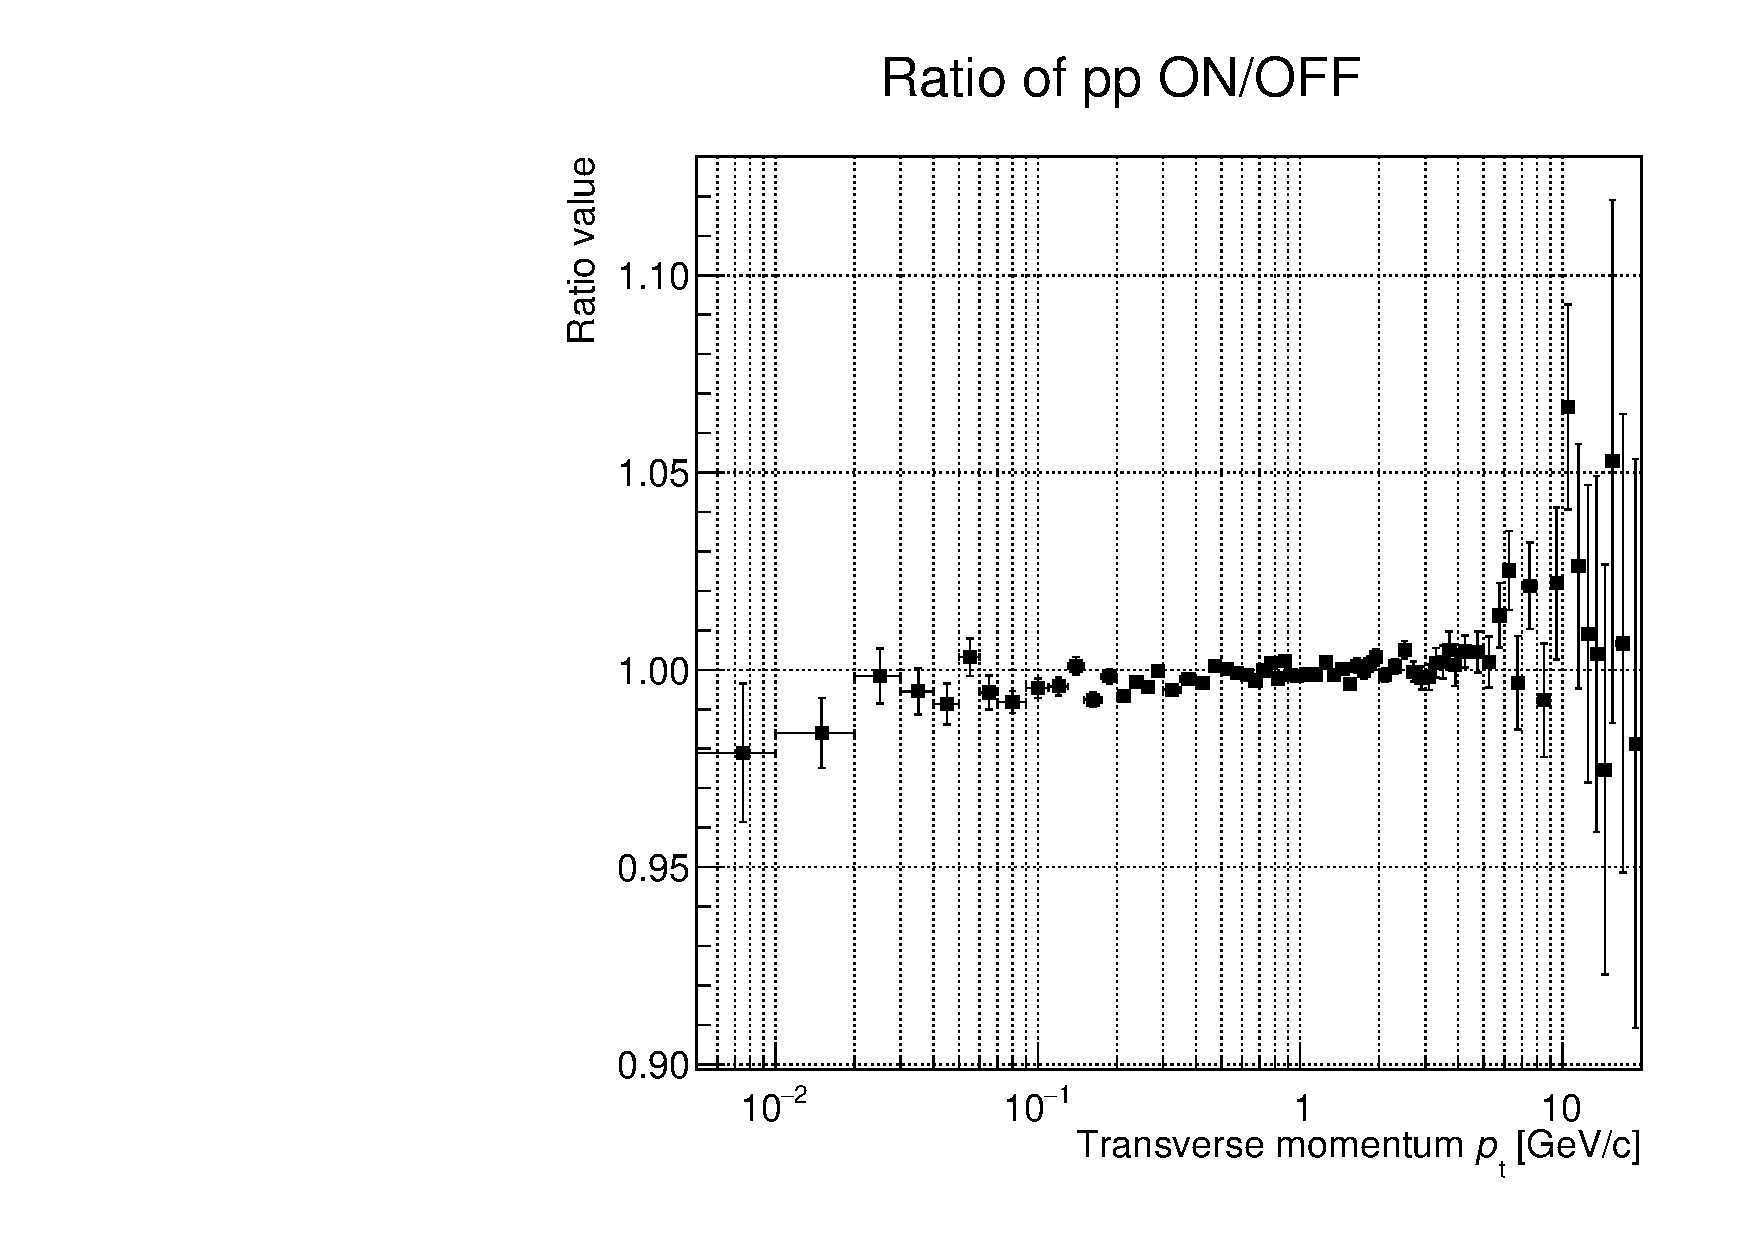
\includegraphics[width=\textwidth]{image/3-risultati/analyse/E/ratio_pp_ON_OFF.pdf}
        \caption{}
        \label{fig:E_ratio_pp_ON_OFF}
    \end{subfigure}
    \captionwithsource{\emph{\rmfamily (a)} Distribuzione dell'impulso trasverso di $p+\bar p$ con produzione deuteronica attivata e disattivata ("ON" e "OFF") in confronto con i dati sperimentali di ALICE ("ALICE"), usando il modello di coalescenza. \emph{\rmfamily (b)} Frazione della distribuzione dell'impulso trasverso di $p+\bar p$ con produzione deuteronica attivata e con produzione non attivata, usando il modello di coalescenza.}{\cite{ALICE:2020jsh}}
    \label{fig:E_pp_prod}
\end{figure}
Neanche la divisione tra il caso in cui la produzione deuteronica sia attivata e quella disattivata presenta particolari differenze, come si può notare in \autoref{fig:E_ratio_pp_ON_OFF}, con un valore della media pesata di $0.99873 \pm 0.00023$, vicino al valore di 0.999.

Invece gli spettri di produzione dei (anti)deuteroni (\autoref{fig:E_(anti)deuteron}) hanno un andamento diverso, come deve essere, visto che i diversi modelli utilizzati sono differenti.
Da questi grafici si osserva un andamento discordante degli spettri per tutto il dominio dei dati di ALICE, sottolineando l'inadeguatezza del modello di coalescenza. 
Eseguendo una divisione tra i dati dei (anti)deuteroni di \pythia{} e di ALICE otteniamo il grafico riportato in \autoref{fig:E_division} ed eseguendo una media pesata del rapporto otteniamo il valore di $0.793 \pm 0.012$ per i deuteroni e $0.738 \pm 0.016$ per gli antideuteroni, quindi una sottoproduzione di circa 20-30\%.\\

Come verifica ulteriore della correttezza delle predizioni è stato misurato il rapporto tra gli istogrammi dei deuteroni e degli antideuteroni (\autoref{fig:E_ratio_DD}), ottenendo un valore della media pesata di $1.008 \pm 0.008$, compatibile con il valore unitario.\\

Ora, eseguendo invece una divisione tra il modello di coalescenza e il modello predefinito di \pythiaa{}, si ottiene il grafico visibile in \autoref{fig:A_vs_E}.
I due modelli presentano un andamento simile solamente nel range tra $0.1-1$ GeV/$c$, in cui per entrambi si è osservato una sovrapproduzione di (anti)deuteroni rispetto ai dati di ALICE.
\begin{figure}[htbp]
    \centering
    \begin{subfigure}{.49\textwidth}
    \centering
        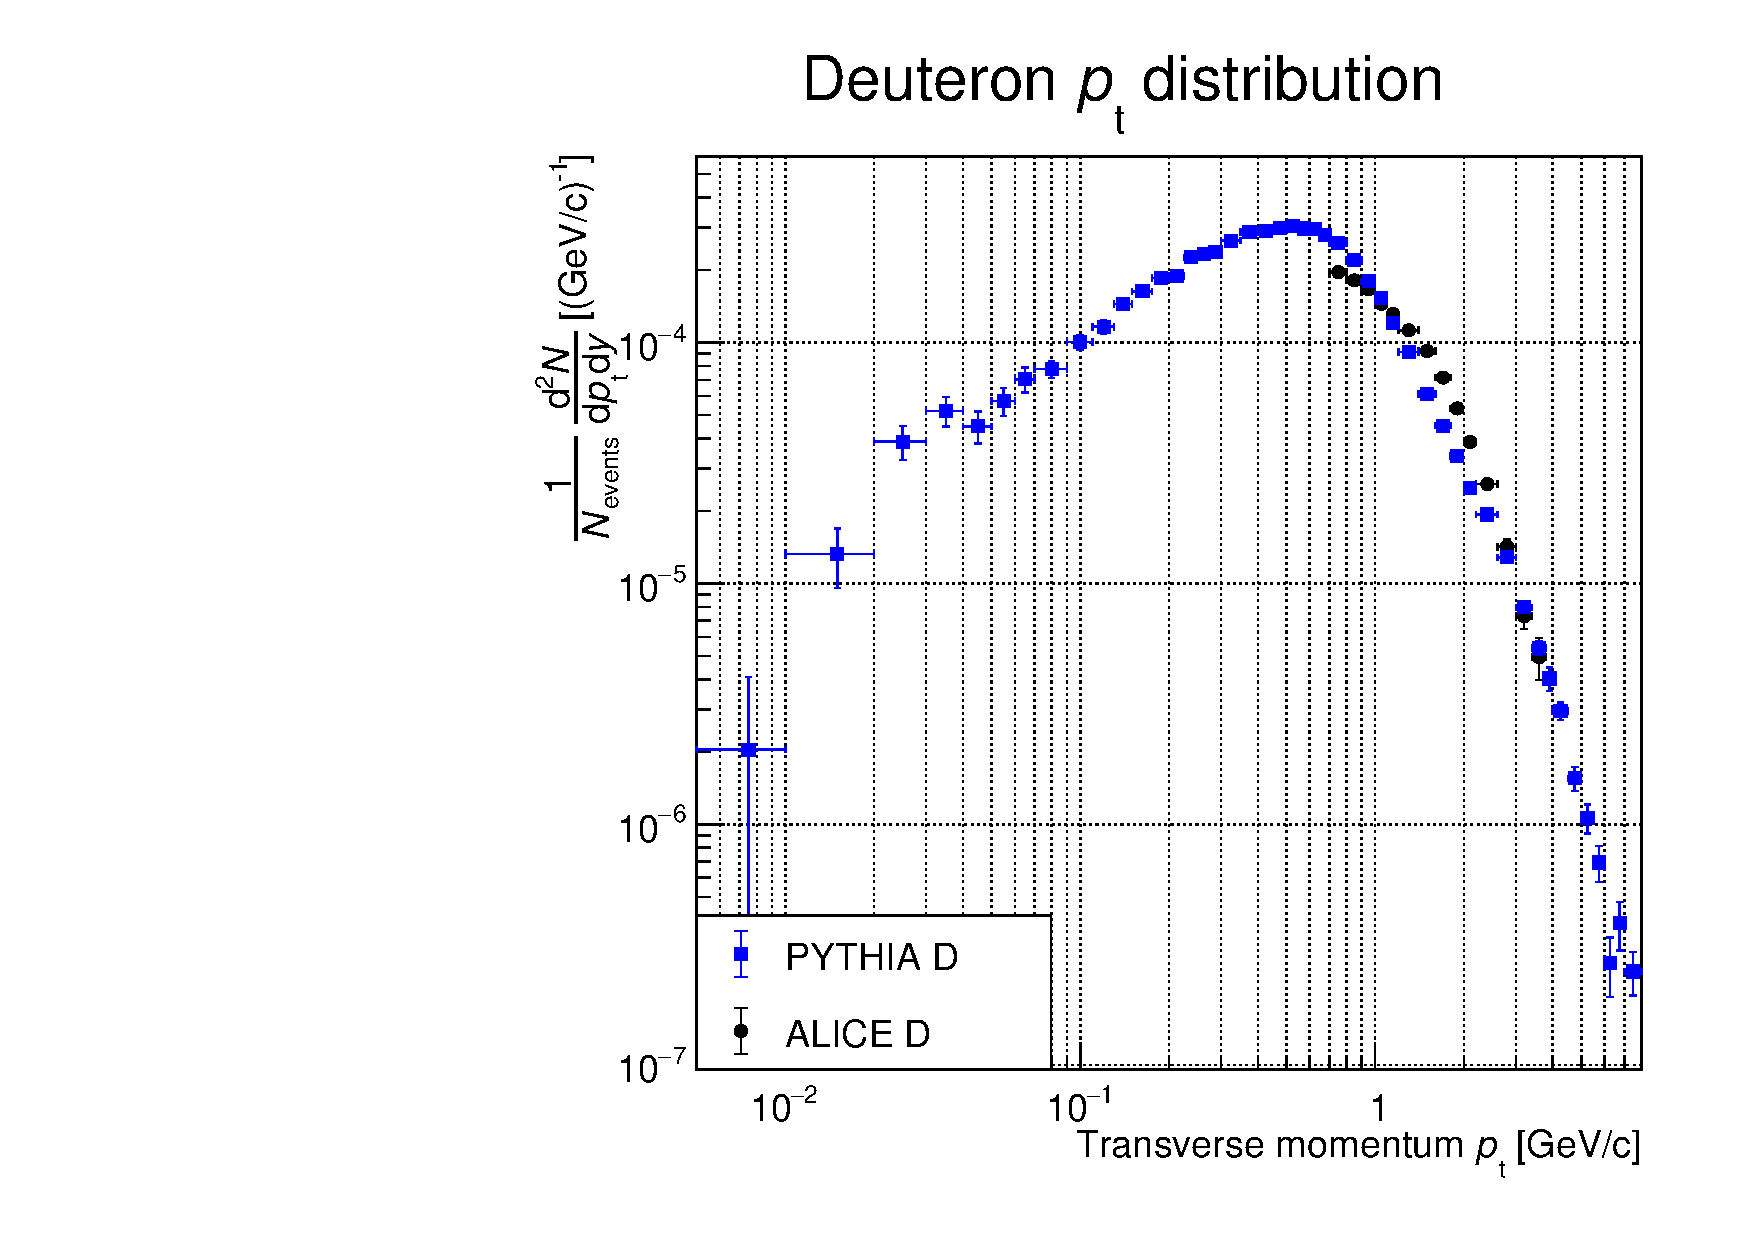
\includegraphics[width=\textwidth]{image/3-risultati/analyse/E/deuteron.pdf}
        \caption{}
        \label{fig:E_deuteron}
    \end{subfigure}
    %\hspace{1cm}
    \begin{subfigure}{.49\textwidth}
        \centering
        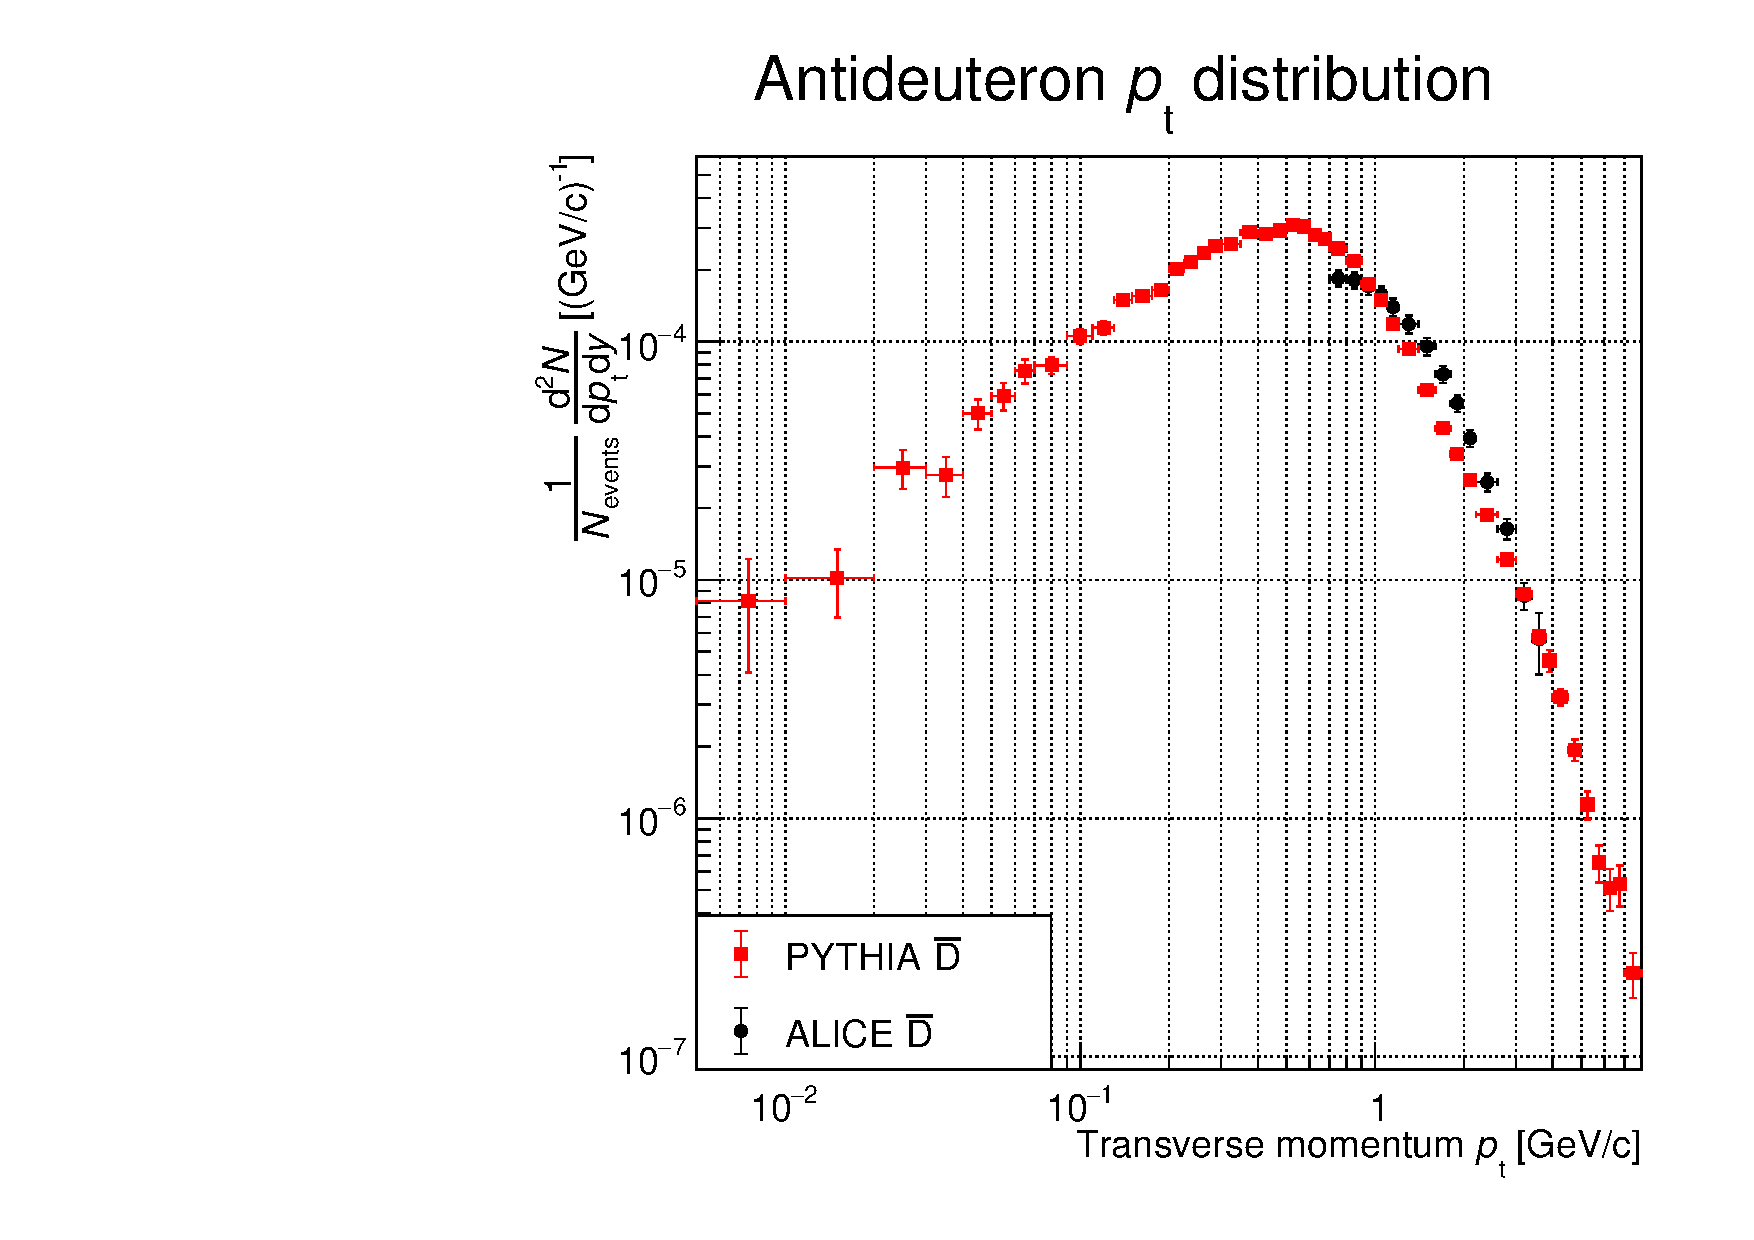
\includegraphics[width=\textwidth]{image/3-risultati/analyse/E/antideuteron.pdf}
        \caption{}
        \label{fig:E_antideuteron}
    \end{subfigure}
    \captionwithsource{Distribuzione dell'impulso trasverso di \emph{\rmfamily (a)} $D$ e \emph{\rmfamily (b)} di $\bar D$ in confronto con i dati di ALICE, utilizzando il modello di coalescenza.}{\cite{ALICE:2020foi}}
    \label{fig:E_(anti)deuteron}
\end{figure}
\begin{figure}[htbp]
    \centering
    \begin{subfigure}{.49\textwidth}
    \centering
        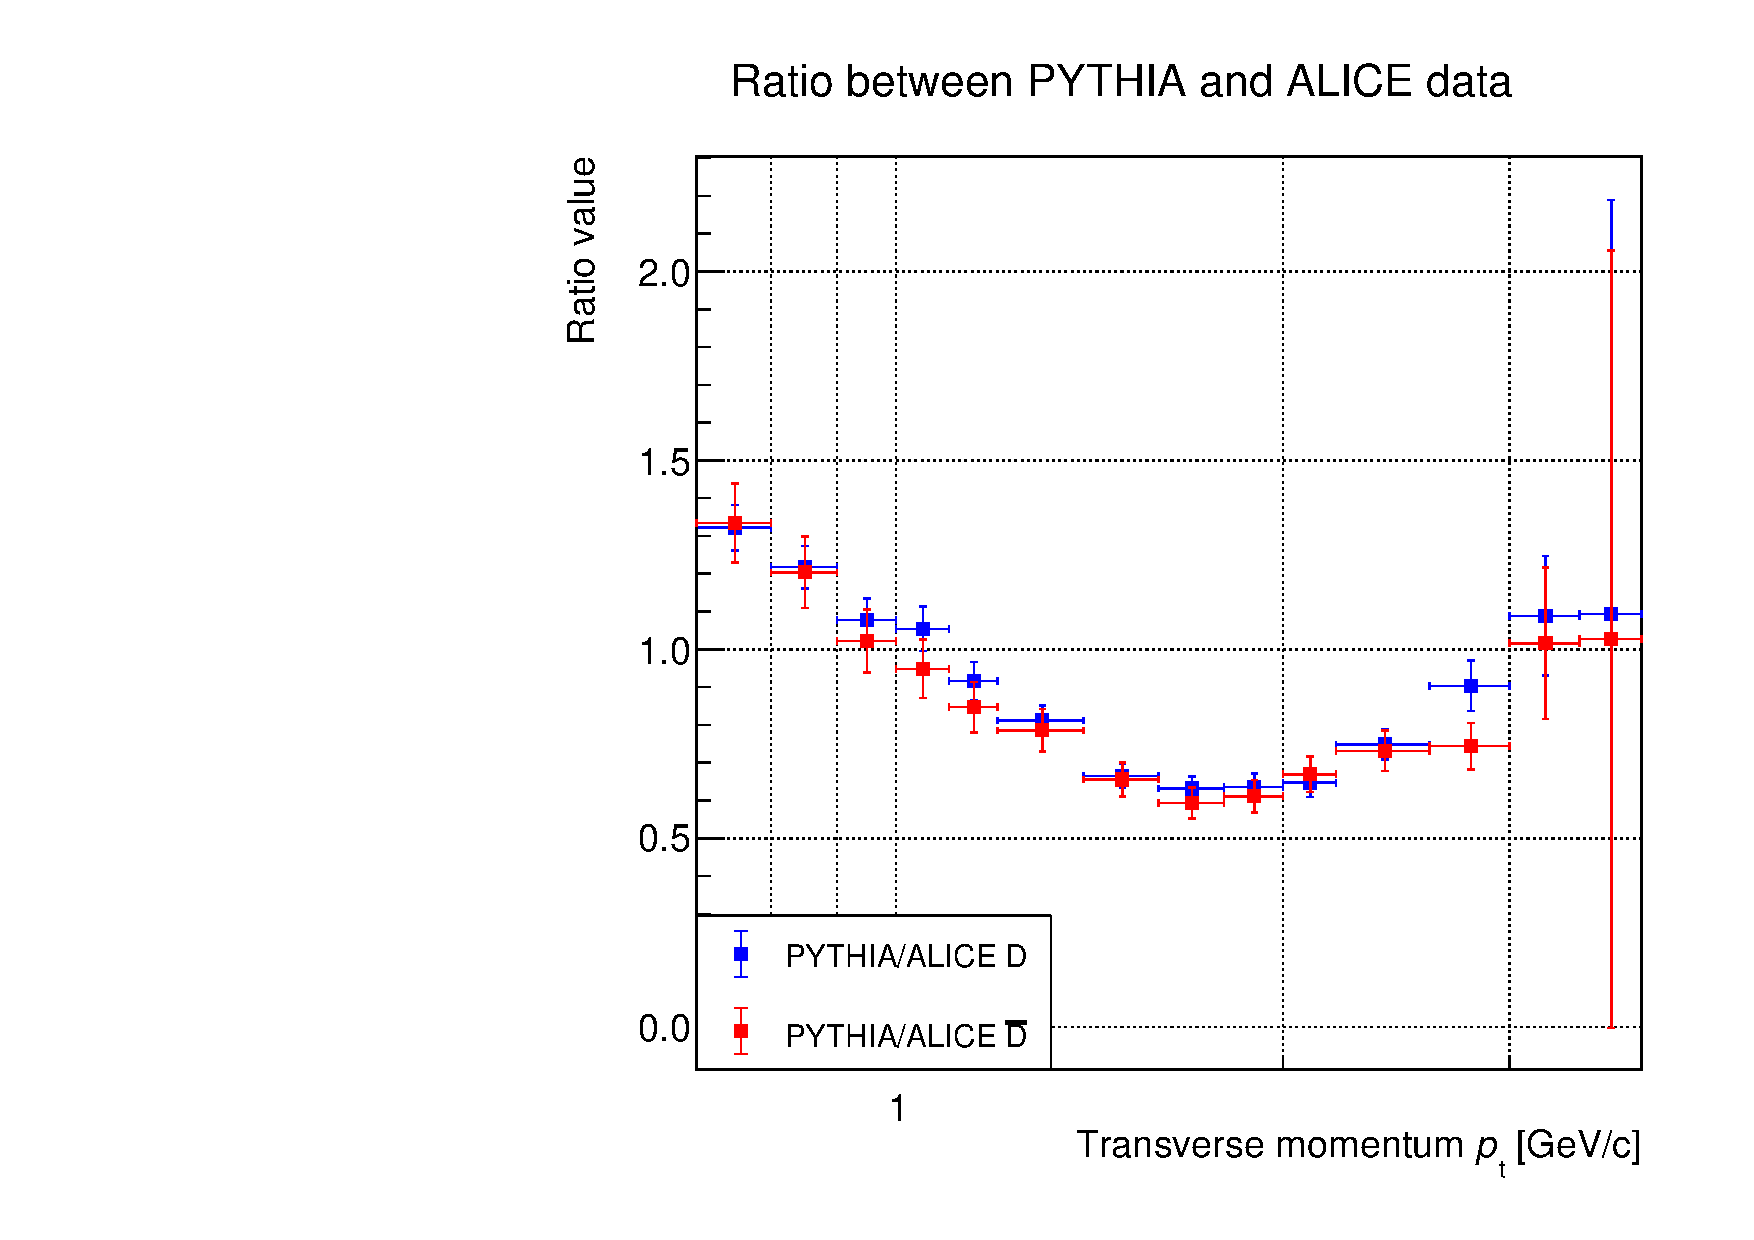
\includegraphics[width=\textwidth]{image/3-risultati/analyse/E/division.pdf}
        \caption{}
        \label{fig:E_division}
    \end{subfigure}
    %\hspace{1cm}
    \begin{subfigure}{.49\textwidth}
        \centering
        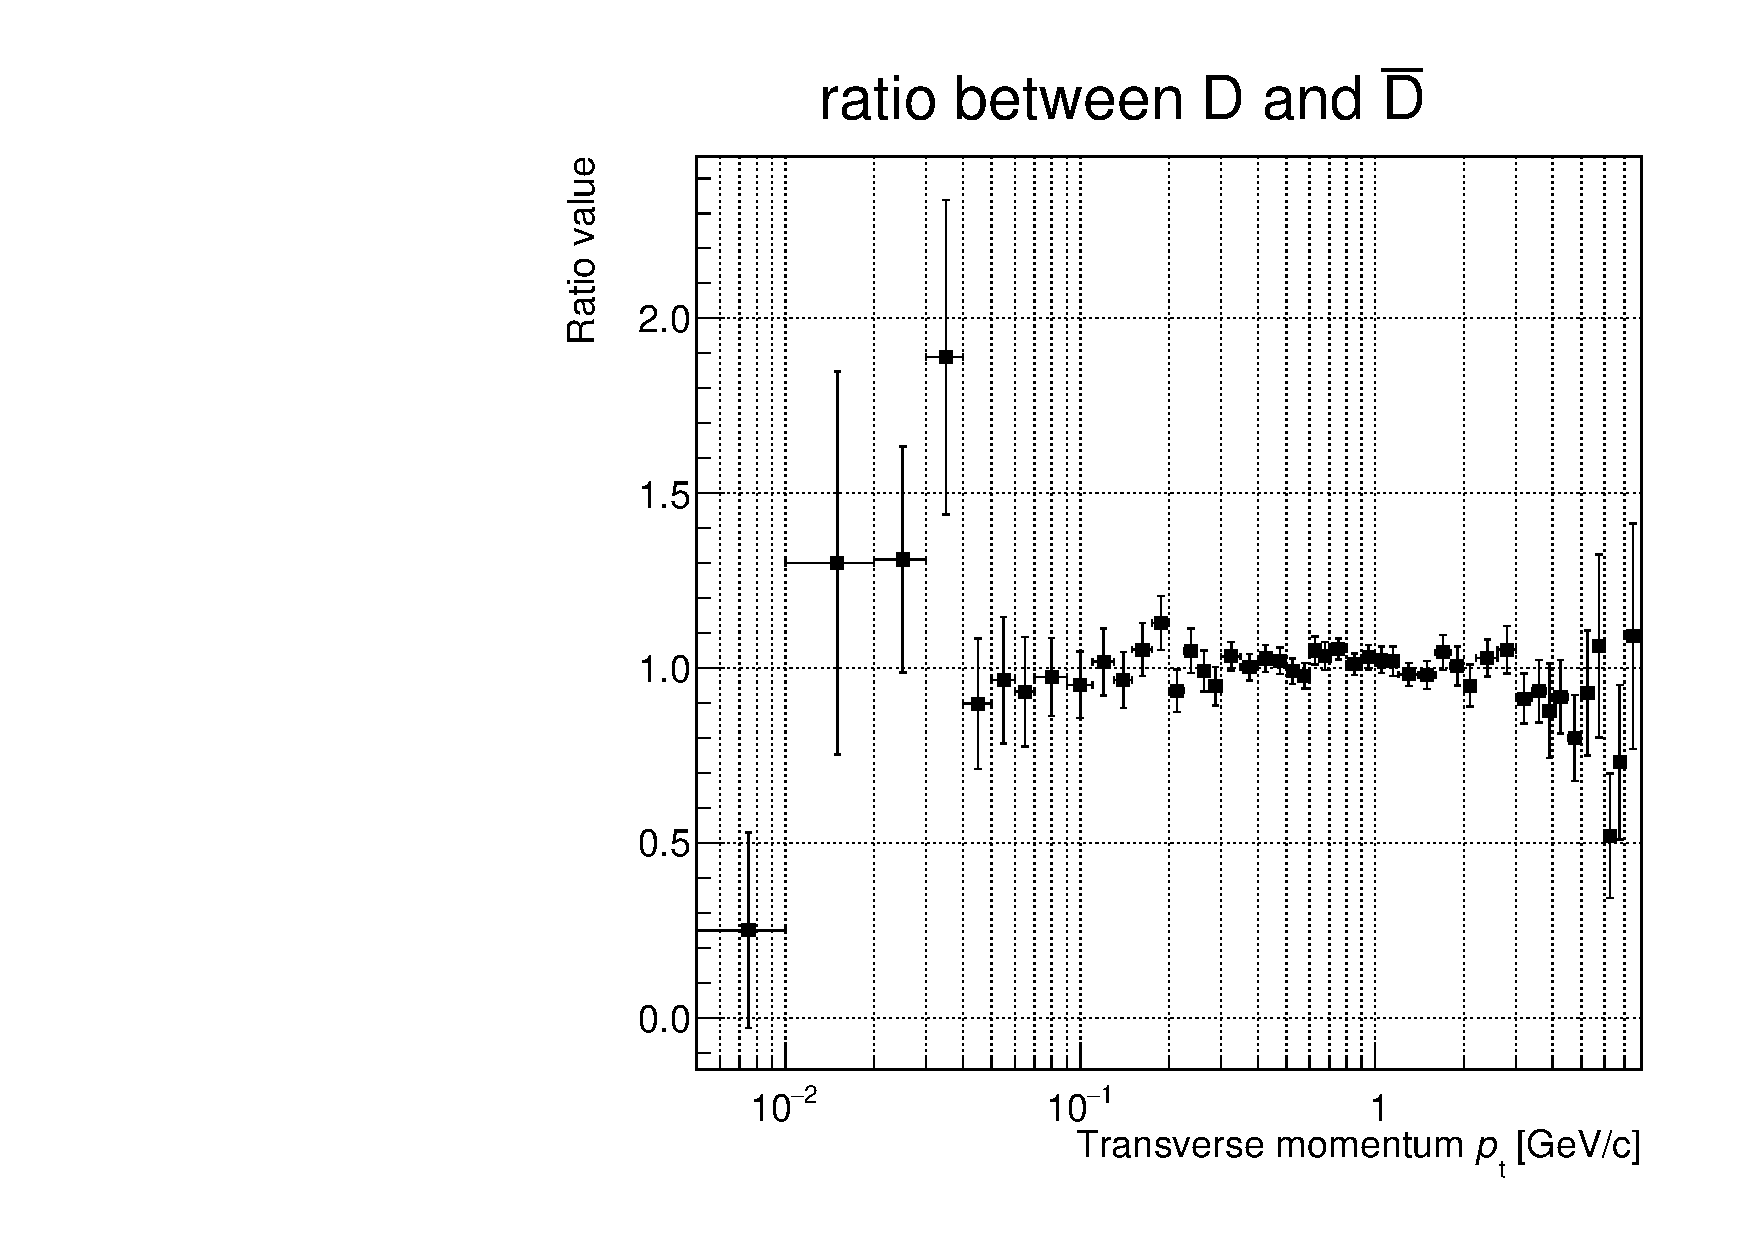
\includegraphics[width=\textwidth]{image/3-risultati/analyse/E/ratio_DD.pdf}
        \caption{}
        \label{fig:E_ratio_DD}
    \end{subfigure}
    \caption{\emph{\rmfamily (a)} Divisione tra la distribuzione dell'impulso trasverso di $D$ e $\bar D$ con i dati di ALICE, utilizzando il modello di coalescenza. \emph{\rmfamily (b)} Frazione delle distribuzione dell'impulso trasverso di $D$ con quello di $\bar D$, utilizzando il modello di coalescenza.}
    \label{fig:E_ratio_DD_}
\end{figure}
\begin{figure}[htp]
    \centering
    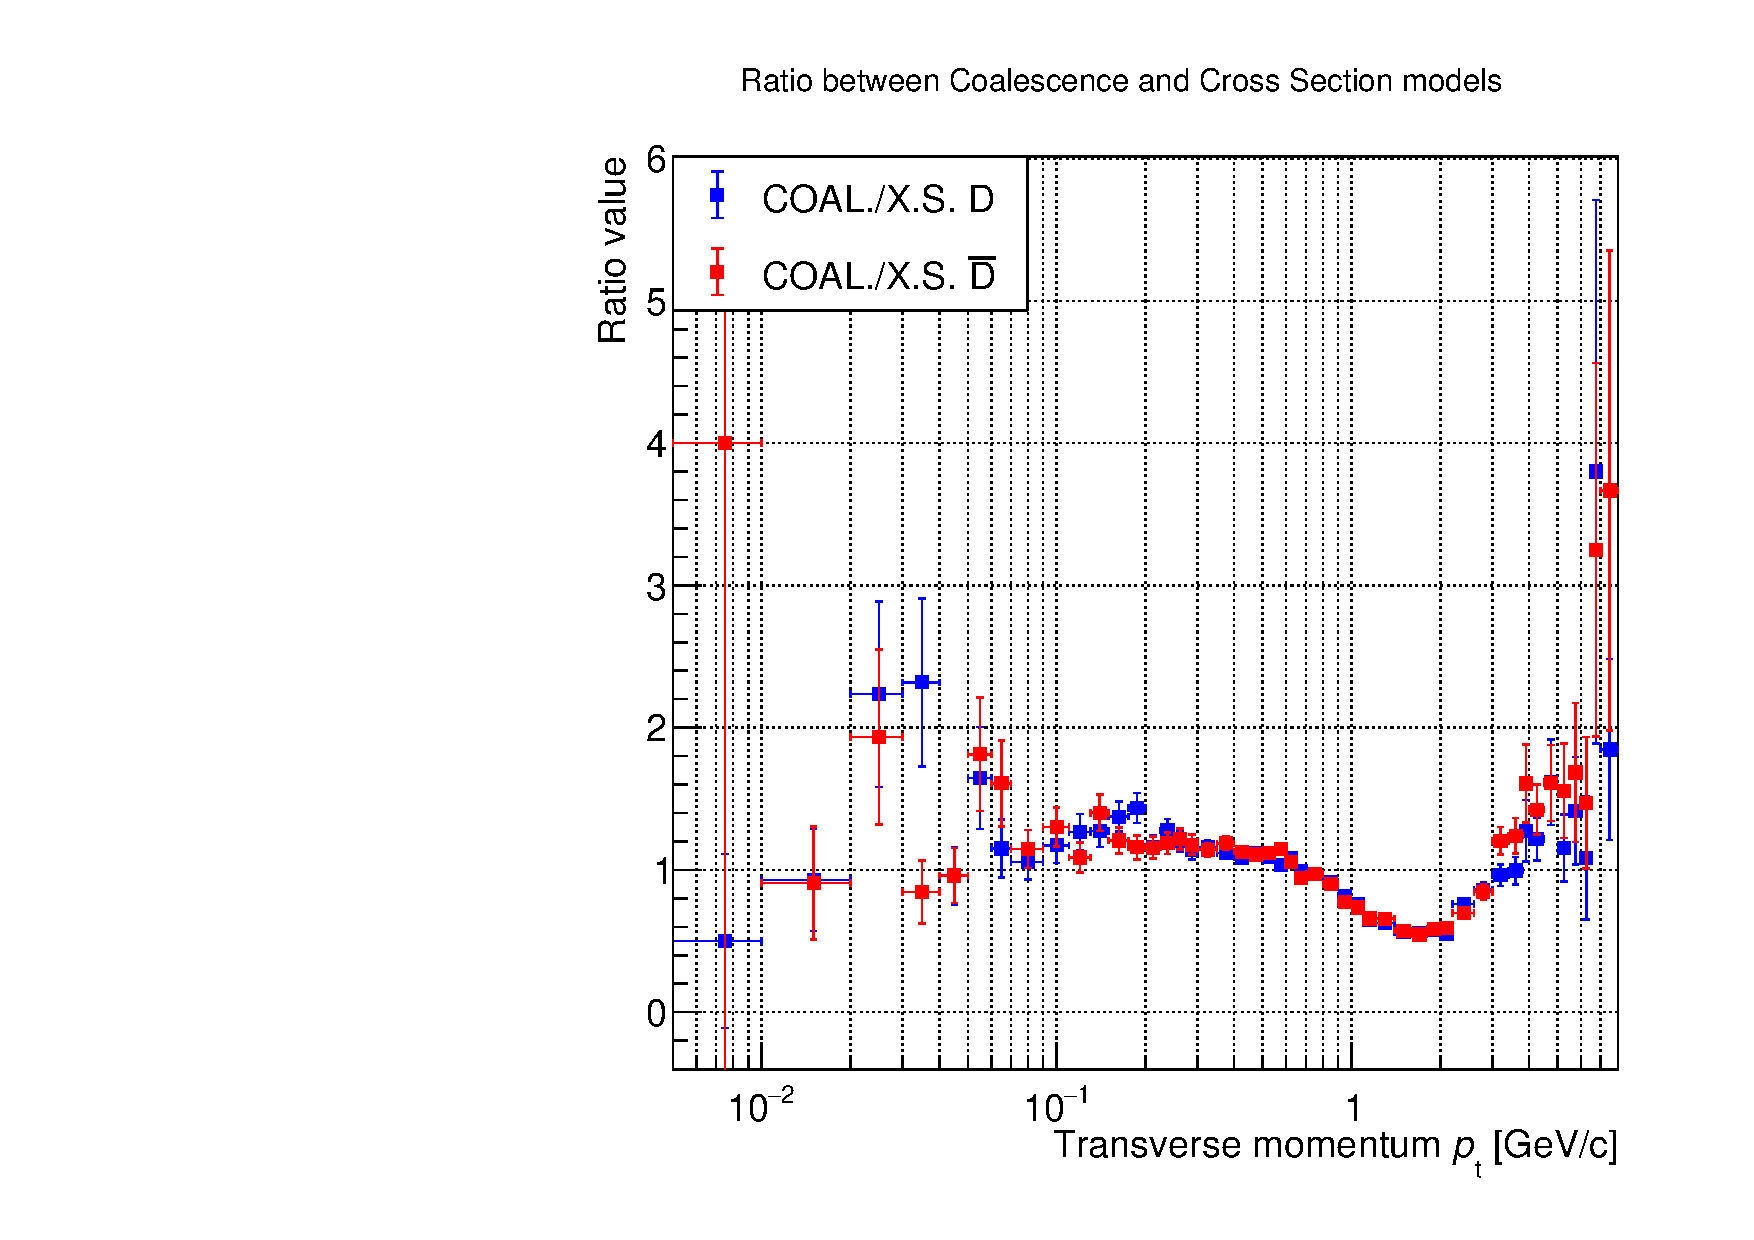
\includegraphics[width=0.49\textwidth]{image/3-risultati/analyse/A/ratio_CXS.pdf}
    \caption{Rapporto tra la distribuzione dell'impulso trasverso di $D$ e $\bar D$ ottenuta con il modello di coalescenza e con il modello predefinito di \emph{\pythiaa}. "COAL" indica il modello di coalescenza, "X.S." indica il modello di \pythiaa{}.}
    \label{fig:A_vs_E}
\end{figure}
%%%%%%%%%%%%%%%%%%%%%%%%%%%%%%%%%%%%%%%%%%
\section{Ottimizzazione del modello di PYTHIA}
Il lavoro principale di questa tesi è stato quello di andare a ottimizzare il parametro \ttbox{norm}.
Originariamente il gruppo di \pythiaa{} aveva calcolato questo parametro scegliendo il valore di $1/\sigma_0$ con energia di centro di massa $\sqrt s = 7$ TeV per il caso dei deuteroni, ossia $1/\sigma_0 = 2.63$ \si{barn^{-1}} (si veda la \autoref{tab:valori_p0_1sigma0}).
Questo dovrebbe spiegare gli andamenti dei grafici in \autoref{fig:A_(anti)deuteron} che non riproducono fedelmente quelli di ALICE.
Quindi si è andati a prendere in considerazione la \autoref{tab:valori_p0_1sigma0} e a cercare di determinare il valore di $1/\sigma_0$ corrispondente a una energia del centro di massa $\sqrt s = 13$ TeV.
Visto che le impostazioni predefinite hanno prodotto una sovrapproduzione, allora vuol dire che $1/\sigma_0$ ha assunto un valore troppo alto per $\sqrt s = 13$ TeV.
Ciò è supportato dal fatto che $1/\sigma_0$ ha un andamento decrescente nella \autoref{tab:valori_p0_1sigma0}.
Quindi l'obiettivo è stato quello di estrapolare questo parametro dalla tabella in questione, facendo attenzione al numero ridotto di punti che si ha a disposizione.

\subsubsection{Fit lineare}
Un primo approccio è stato quello di effettuare un fit lineare ai dati del deuterone per cercare di ottenere un valore preliminare tramite il quale andare a raffinare il parametro.
Tramite questo fit lineare (\autoref{fig:fit_norm}) l'estrapolazione di $1/\sigma_0$ a $\sqrt{s} = 13$ TeV fornisce un valore di $1.7136$ \si{barn^{-1}}, con un valore di $\ttbox{norm} = 183.56$.
\begin{figure}[htb]
    \centering
    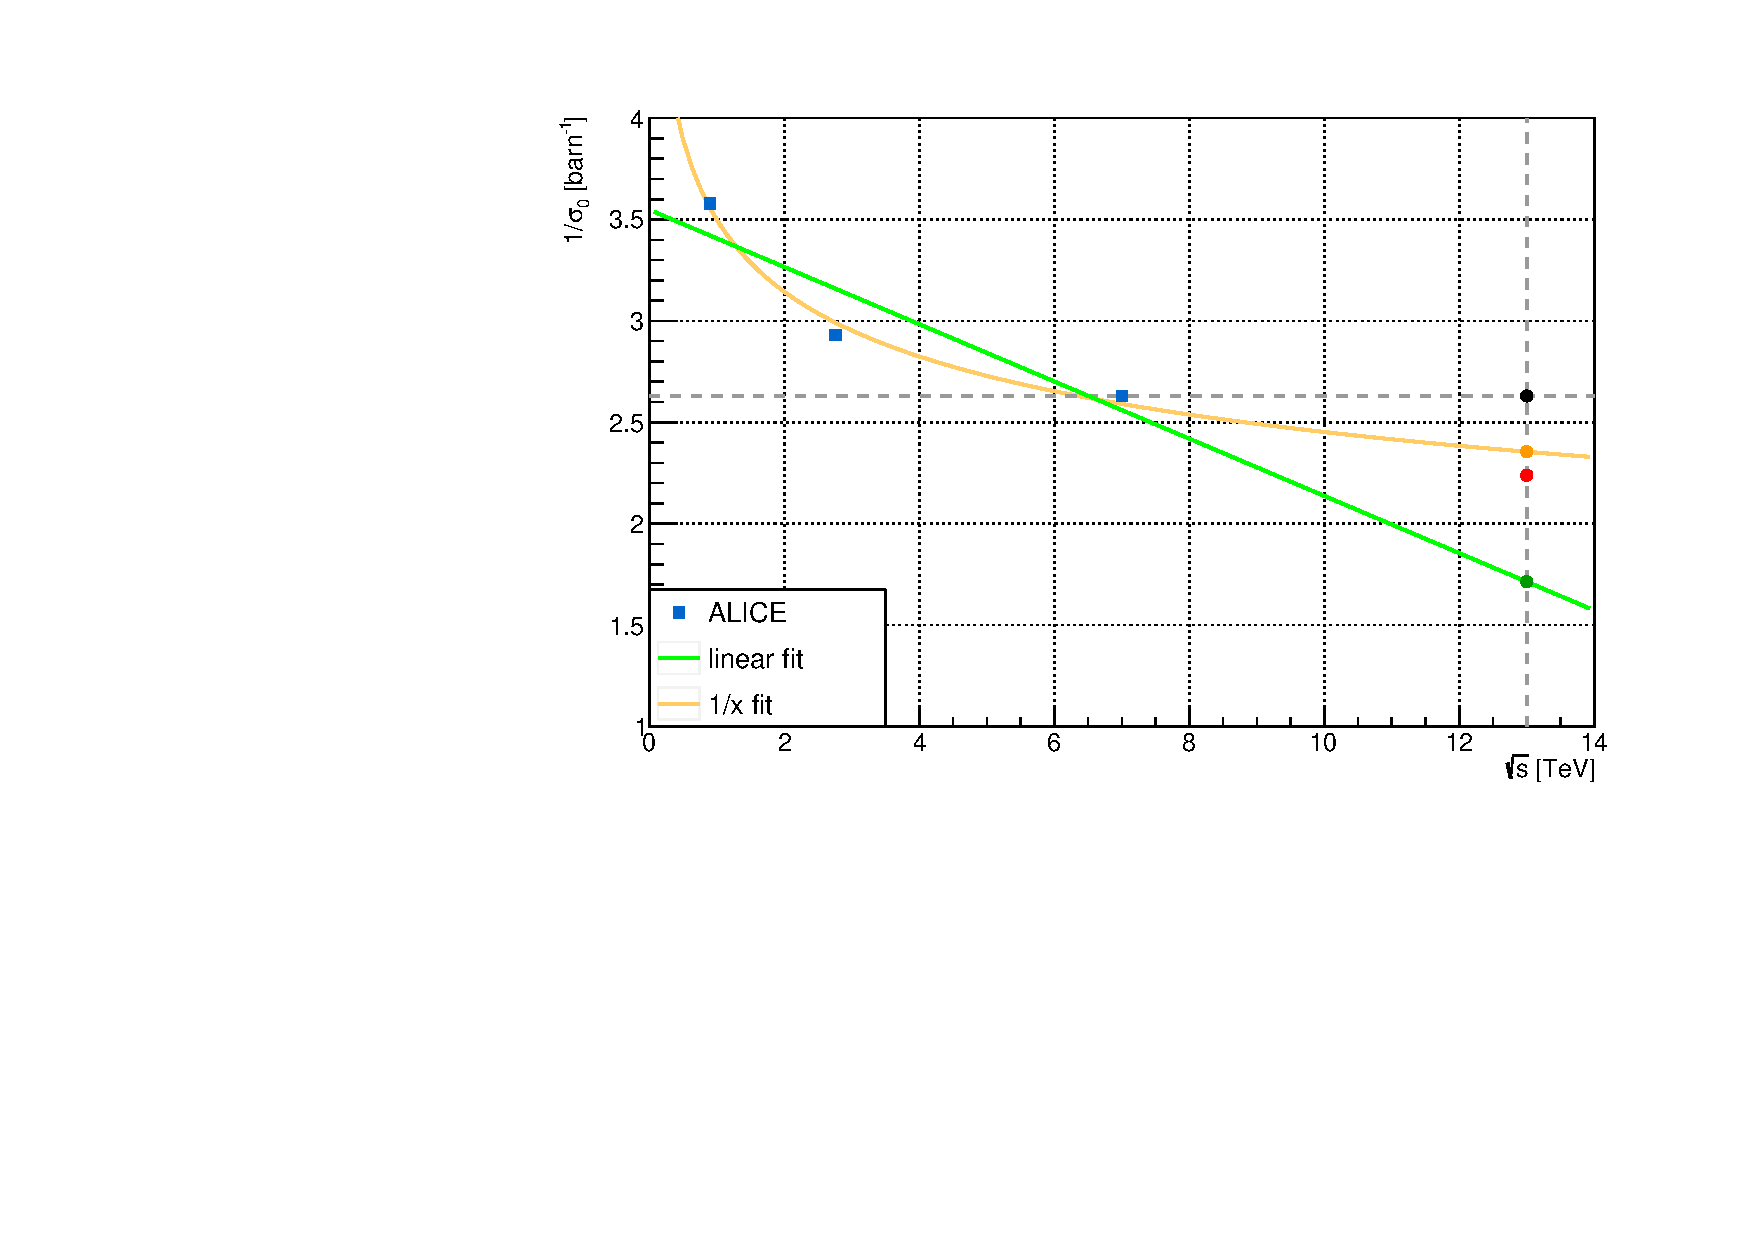
\includegraphics[width=0.9\textwidth]{image/canvas.pdf}
    \caption{Risultati del fit lineare e $1/x$ del parametro $1/\sigma_0$ per i deuteroni. La retta tratteggiata in orizzontale rappresenta $1/\sigma_0 = 2.63$ \si{barn^{-1}}, quella verticale $\sqrt s = 13$ TeV. Su quest'ultima vi sono quattro punti, che in ordine rappresentano (dall'alto verso il basso) il parametro default, del fit $1/x$, ottimizzato e del fit lineare.
    "ALICE" indica i punti derivati da \autoref{tab:valori_p0_1sigma0} nella colonna dei deuteroni.}
    \label{fig:fit_norm}
\end{figure}
Per verificare l'attendibilità di questo valore si è andati a effettuare una simulazione con questo valore di \ttbox{norm} e a confrontare lo spettro di produzione dei (anti)deuteroni con quelli di ALICE.
Le medie pesate derivate dai rapporti tra i dati di \pythiaa{} e di ALICE (in \autoref{fig:B_division}) hanno portato a un valore di $0.789 \pm 0.012$ e $0.746 \pm 0.016$ rispettivamente per i deuteroni e per gli antideuteroni, indicando una sottoproduzione del circa 20-25\%.
Da ciò si può dedurre che il valore $1/\sigma_0$ estrapolato tramite un fit lineare è inferiore rispetto al parametro ideale.
Un fit analogo del parametro $1/\sigma_0$ per gli antideuteroni ha fornito un valore di $1.56872$ \si{barn^{-1}}, corrispondente a $\ttbox{norm} = 200.51$, che tuttavia risulta troppo alto visto il risultato della simulazione con $\ttbox{norm} = 183.56$; tale valore perciò non è stato considerato.

\subsubsection{Fit ${\bf 1/x}$}
Un secondo approccio più realistico è stato quello di tentare di fittare i tre punti con una funzione del tipo
\begin{equation}
    1/\sigma_0\left(\sqrt s\right) = \dfrac{a}{x^b}
\end{equation}
Eseguendo il fit (\autoref{fig:fit_norm}) con questa funzione si è riusciti a ottenere i seguenti valori dei parametri di fit: $a = (3.50 \pm 0.07)$ \si{barn^{-1}} e $b = 0.154 \pm 0.017$.
Così il valore di $1/\sigma_0$ estrapolato a $\sqrt s = 13$ TeV risulta essere di $2.35473$ \si{barn^{-1}}, quindi $\ttbox{norm} = 133.58$, valore accettabile perché compreso tra 119.6 e 183.56.
Eseguendo le simulazioni Monte Carlo con questo parametro si ottiene che gli andamenti degli spettri dei (anti)deuteroni si avvicinano di più ai dati di ALICE rispetto alle simulazioni precedenti.
\begin{figure}[h]
    \centering
    \begin{subfigure}{.49\textwidth}
    \centering
        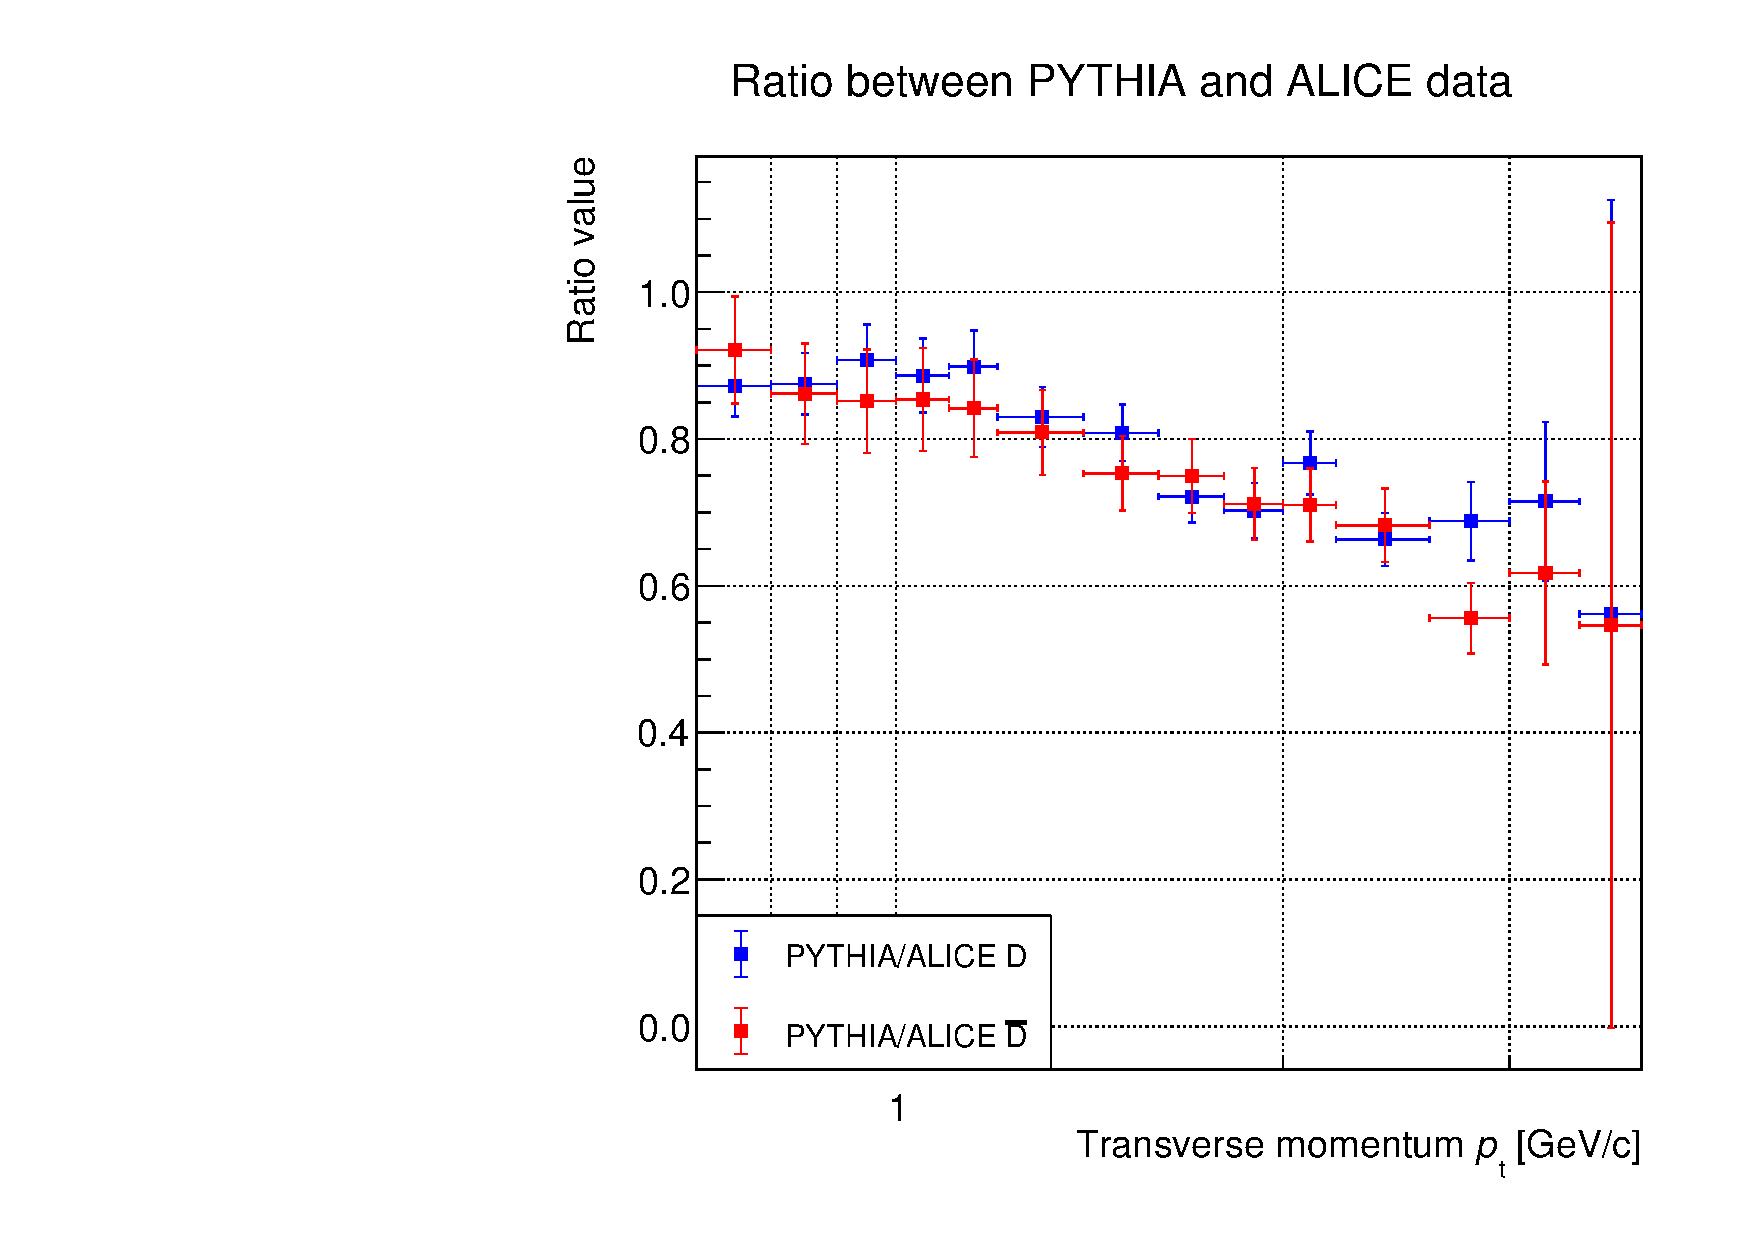
\includegraphics[width=\textwidth]{image/3-risultati/analyse/B/division.pdf}
        \caption{}
        \label{fig:B_division}
    \end{subfigure}
    %\hspace{1cm}
    \begin{subfigure}{.49\textwidth}
        \centering
        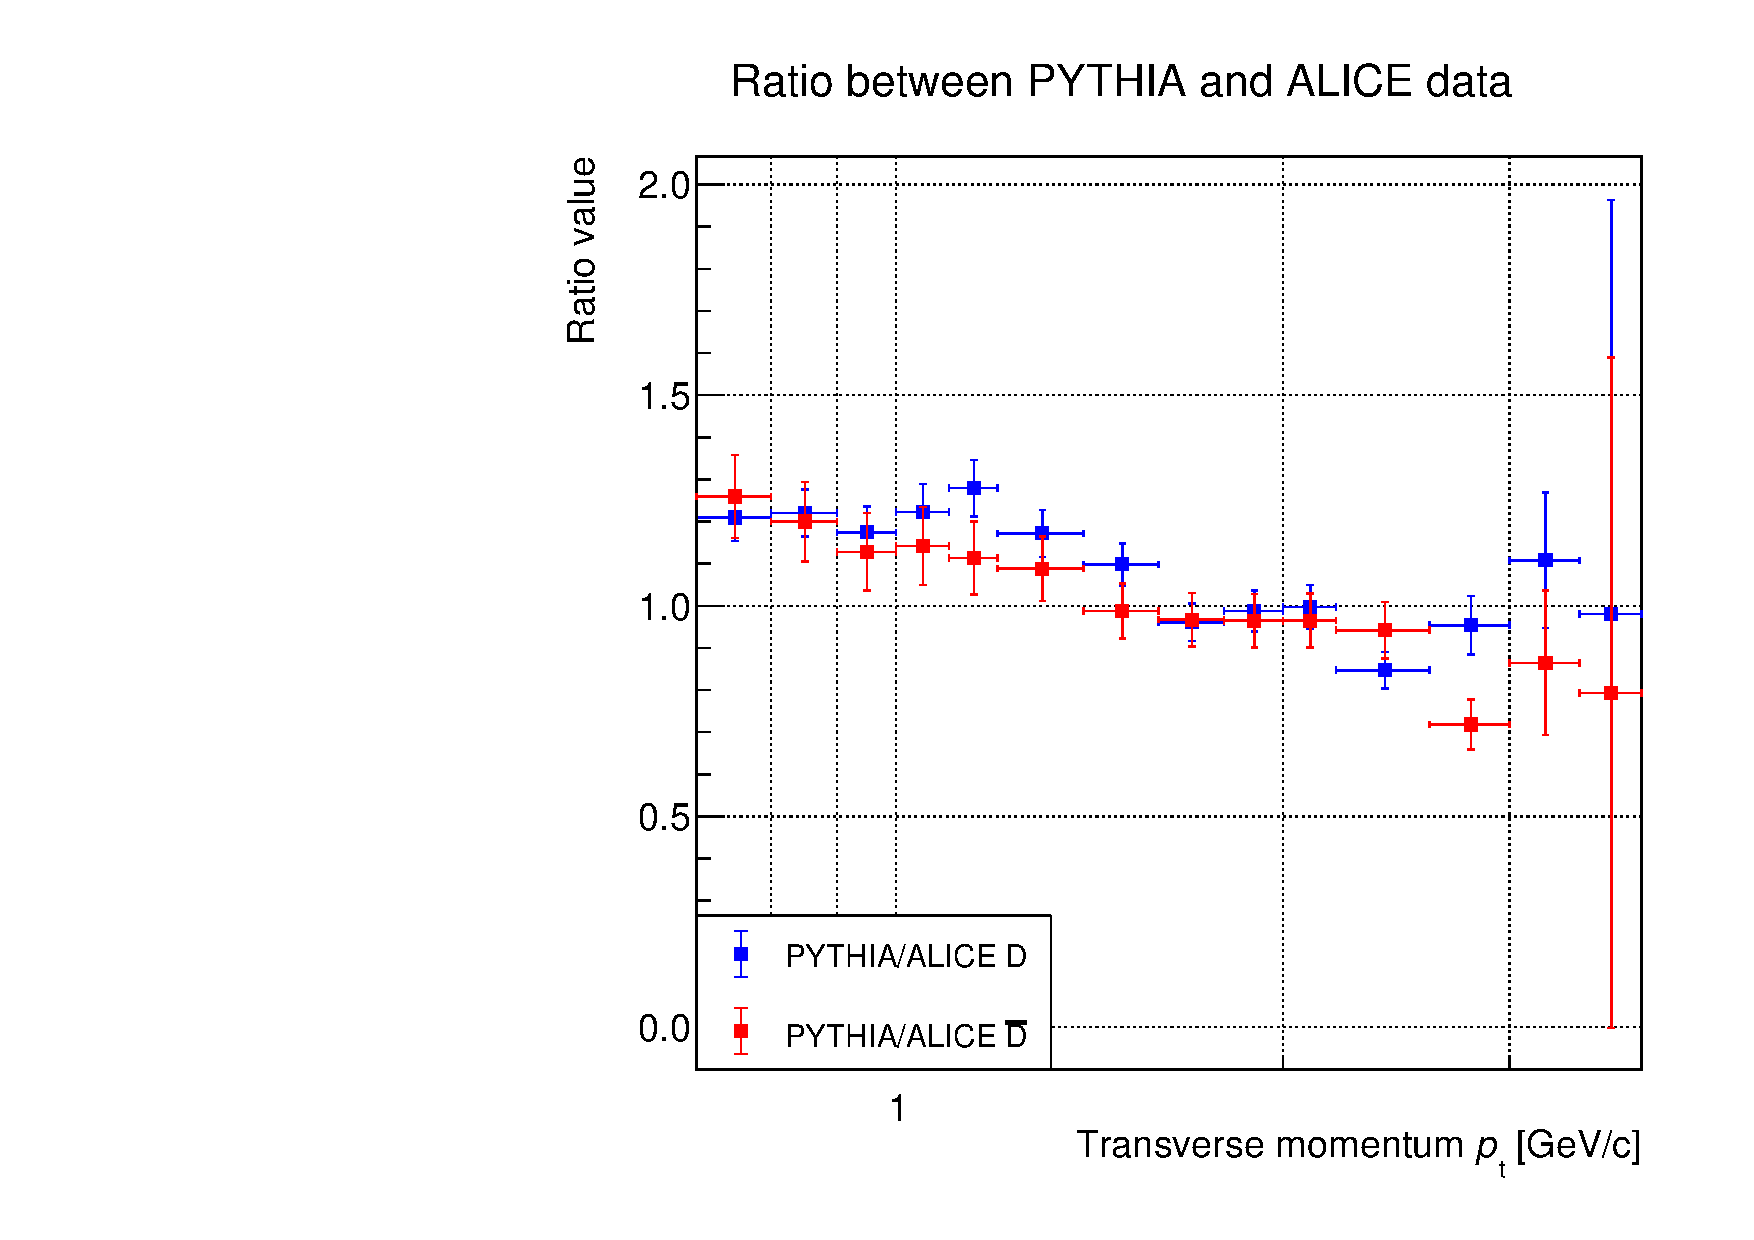
\includegraphics[width=\textwidth]{image/3-risultati/analyse/F/division.pdf}
        \caption{}
        \label{fig:F_division}
    \end{subfigure}
    \caption{Rapporto tra la distribuzione dell'impulso trasverso di $D$ e $\bar D$ con i dati di ALICE \emph{\rmfamily (a)} con \emph{\ttbox{norm}}$=183.56$ e \emph{\rmfamily (b)} con \emph{\ttbox{norm}}$=133.58$.}
    \label{fig:ratio_pp_ON_OFF_BF}
\end{figure}
Questo è supportato dal valore della media pesata del rapporto tra lo spettro dei (anti)deuteroni con i dati di ALICE (\autoref{fig:F_division}) che vale $1.067 \pm 0.015$ e di $0.993 \pm 0.021$ rispettivamente per i deuteroni e per gli antideuteroni. Quindi si nota che il valore di \ttbox{norm} per gli antideuteroni risulta già compatibile entro gli errori con il valore unitario, ma non per i deuteroni.
Questo valore del parametro potrebbe apparire come valore  ottimale, ma ricordando che i valori considerati della \autoref{tab:valori_p0_1sigma0} si riferiscono solamente ai deuteroni, perciò si è proseguiti con l'ottimizzazione del parametro.

\subsubsection{Bisezione}
Per trovare un valore del parametro \ttbox{norm} tale da soddisfare sia la produzione di deuteroni e antideuteroni si è proceduti con un altro metodo alternativo, ispirato al metodo di bisezione.
Per far ciò si correla il parametro \ttbox{norm} con la relativa media pesata.
Andando a considerare i punti del modello predefinito ($\ttbox{norm} = 119.6$, media pesata $= 1.203 \pm 0.017$) e del fit $1/x$ ($\ttbox{norm} = 133.58$, media pesata $= 1.067 \pm 0.03$), si è andati a stimare il valore ottimale del parametro eseguendo empiricamente un fit lineare dei due punti e ricavare il valore del parametro quando la media assume un valore di 1.
Utilizzando questo approccio si è giunti al valore del parametro di $\ttbox{norm} = 140.46721$, leggermente inferiore al parametro derivato dal fit $1/x$.
Eseguendo le simulazioni Monte Carlo ed effettuando il rapporto tra le produzioni di (anti)deuteroni delle simulazioni e di ALICE, otteniamo i valori di media pesata di $1.036 \pm 0.015$ per i deuteroni e $ 0.939 \pm 0.020$ per gli antideuteroni.
Il valore della media pesata per i deuteroni è vicino a 1, ma non è compatibile entro gli errori.
Tuttavia, per semplicità assumiamo questo valore come valore ideale di \ttbox{norm}, e tramite una formula inversa ricaviamo un valore di $1/\sigma_0$ di 2.24 \si{barn^{-1}}.\\

È doveroso notare che, modificando il parametro \ttbox{norm}, quello che si va a fare non è altro che un un semplice riscalaggio agli spettri dei (anti)deuteroni, senza favorire un particolare canali di produzione della \autoref{tab:valori_p0_1sigma0}.
Per cui l'analisi dei canali (e dei loro subcanali) eseguita in \autoref{ch:channels} dovrebbe valere per tutti i valori di \ttbox{norm} (ignorando le regioni in cui si ha meno statistica poiché si avrebbero più fluttuazioni). 
%%%%%%%%%%%%%%%%%%%%%%%%%%%%%%%%%%%%%%%%
\section{Confronto del modello predefinito e ottimizzato}
Con l'ottimizzazione effettuata nel paragrafo precedente si è andati a effettuare un confronto tra il modello appena ottimizzato e il modello predefinito, utilizzando grafici analoghi a quelli riportati nella \autoref{ch:default}.
Andando a osservare lo spettro di produzione di $p+\bar p$ non dovremmo osservare particolare differenze, come nel modello pedefinito.
Infatti, come visibile in \autoref{fig:D_pp}, osserviamo un andamento praticamente identico a quello di \autoref{fig:A_pp}.
\begin{figure}[htb]
    \centering
    \begin{subfigure}{.49\textwidth}
    \centering
        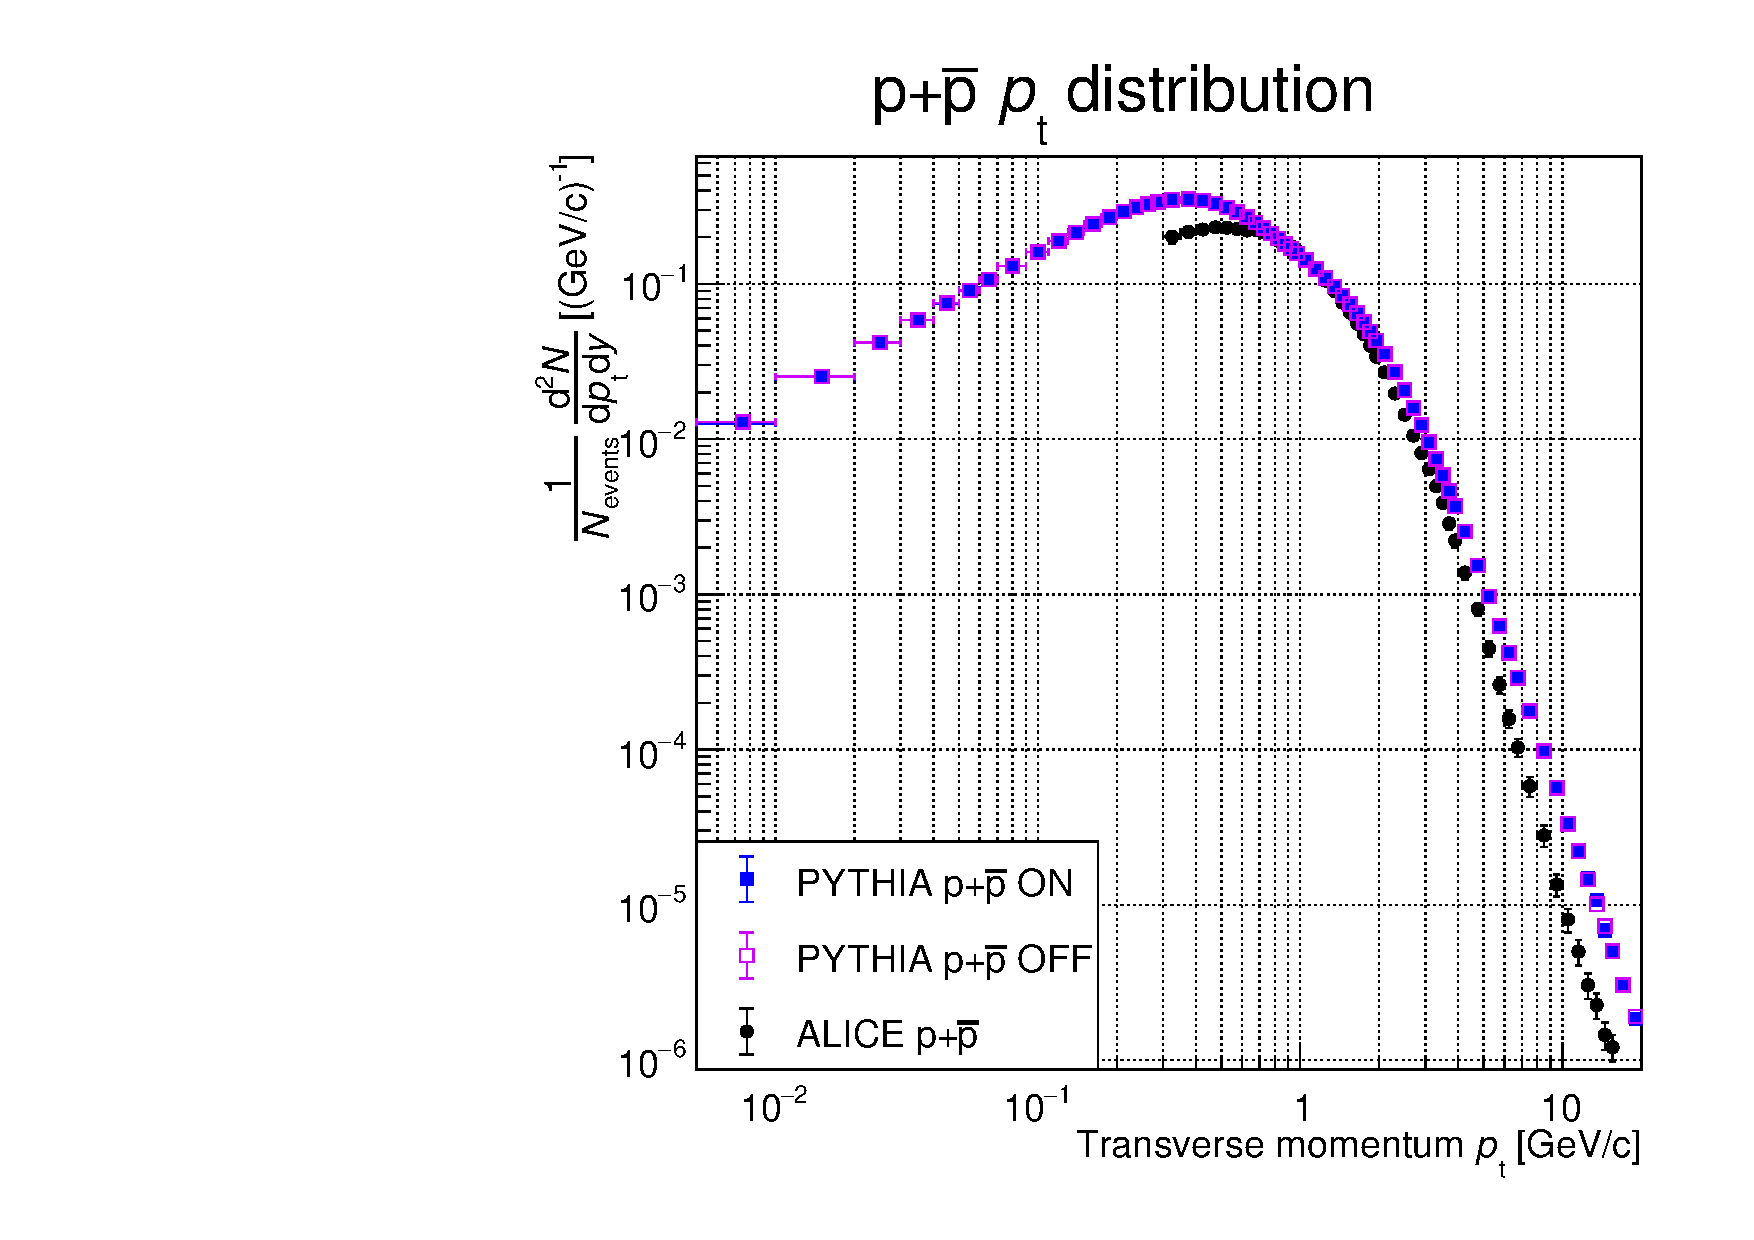
\includegraphics[width=\textwidth]{image/3-risultati/analyse/G/pp.pdf}
        \caption{}
        \label{fig:D_pp}
    \end{subfigure}
    %\hspace{1cm}
    \begin{subfigure}{.49\textwidth}
        \centering
        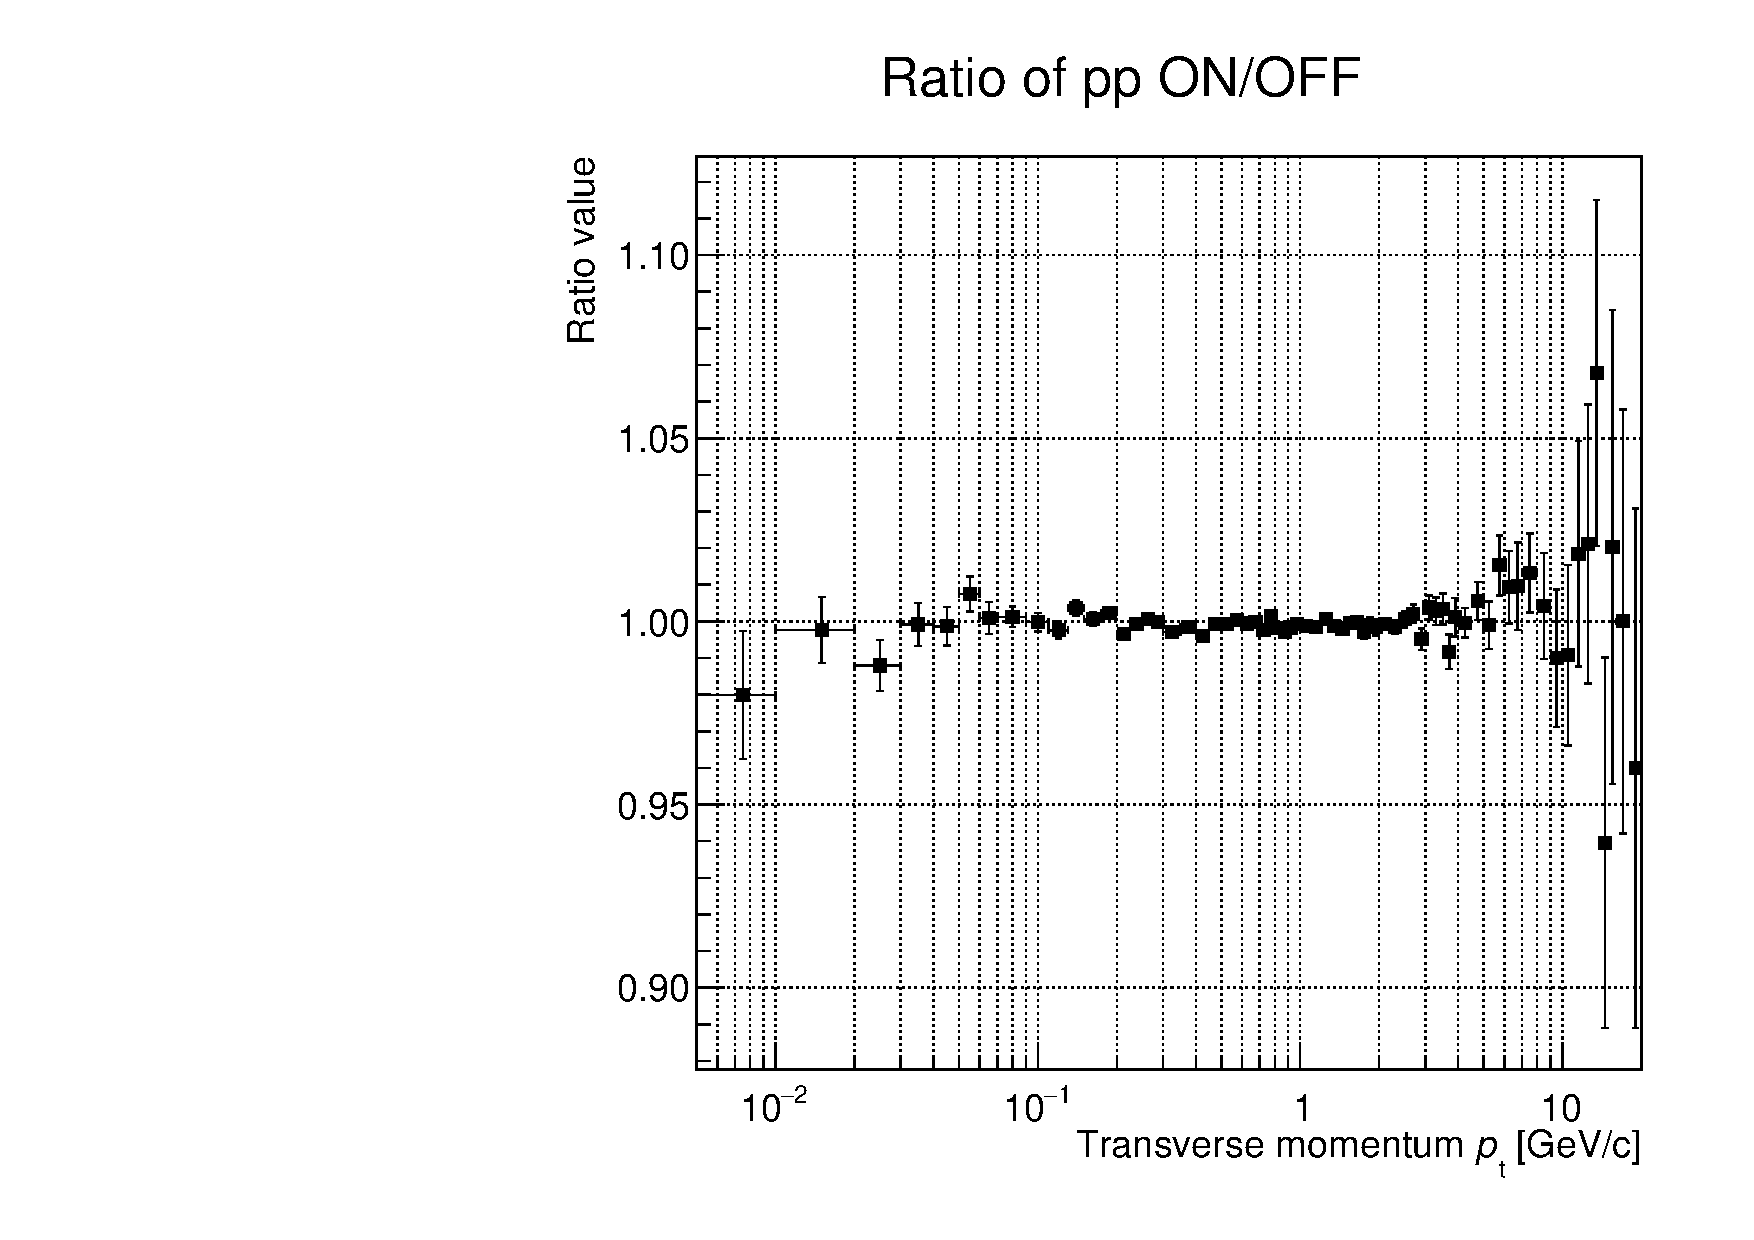
\includegraphics[width=\textwidth]{image/3-risultati/analyse/G/ratio_pp_ON_OFF.pdf}
        \caption{}
        \label{fig:D_ratio_pp_ON_OFF}
    \end{subfigure}
    \captionwithsource{\emph{\rmfamily (a)} Distribuzione dell'impulso trasverso di $p+\bar p$ con produzione deuteronica attivata e disattivata ("ON" e "OFF") in confronto con i dati sperimentali di ALICE ("ALICE"), usando il modello ottimizzato. \emph{\rmfamily (b)} Frazione della distribuzione dell'impulso trasverso di $p+\bar p$ con produzione deuteronica attivata e con produzione non attivata, usando il modello ottimizzato.}{\cite{ALICE:2020jsh}}
    \label{fig:D_pp_prod}
\end{figure}
Neanche il rapporto tra il caso in cui la produzione deuteronica sia attivata e quella disattivata presenta particolari differenze, come si può notare in \autoref{fig:D_ratio_pp_ON_OFF}, con un valore della media pesata di $0.99889 \pm 0.00024$, vicino al valore di 0.999.

Per quanto riguarda gli spettri dei (anti)deuteroni (in \autoref{fig:D_(anti)deuteron}) essi mostrano un accordo migliore con i dati rispetto al modello predefinito, come si può osservare in \autoref{fig:A_(anti)deuteron}.
Ciò è supportato andando a effettuare una divisione tra i dati dei (anti)deuteroni di \pythia{} e di ALICE ottenendo così il grafico riportato in \autoref{fig:D_division}.
Come già anticipato, il valore della media pesata del rapporto è di $1.0467 \pm 0.015$ per i deuteroni e $ 0.968 \pm 0.021$ per gli antideuteroni, più vicini al valore unitario rispetto a quello del modello predefinito.

Anche qui si esegue una verifica della correttezza delle simulazioni andando a vedere il bilancio deuteroni-antideuteroni.
Effettuando una divisione tra gli istogrammi dei deuteroni e degli antideuteroni (\autoref{fig:D_ratio_DD}), si ottiene un valore della media pesata di $1.017 \pm 0.008$, compatibile entro 3 sigma con il valore unitario.\\

Per ultimo si esegue un confronto tra i due modelli.
Si ottiene il grafico visibile in \autoref{fig:def_opt}.
È importante notare come le distribuzioni di produzione di (anti)deuterone in funzione dell'impulso trasverso ottenute con i due modelli abbiano in realtà lo stesso identico andamento ma valori assoluti diversi; ciò è dovuto al fatto che le variazioni del parametro \ttbox{norm} agiscono sul numero complessivo di (anti)deuteroni prodotti in tutti i canali di produzione.
Gli spettri prodotti hanno quindi la medesima forma ma un differente fattore di scala.
\begin{figure}[htp]
    \centering
    \begin{subfigure}{.49\textwidth}
    \centering
        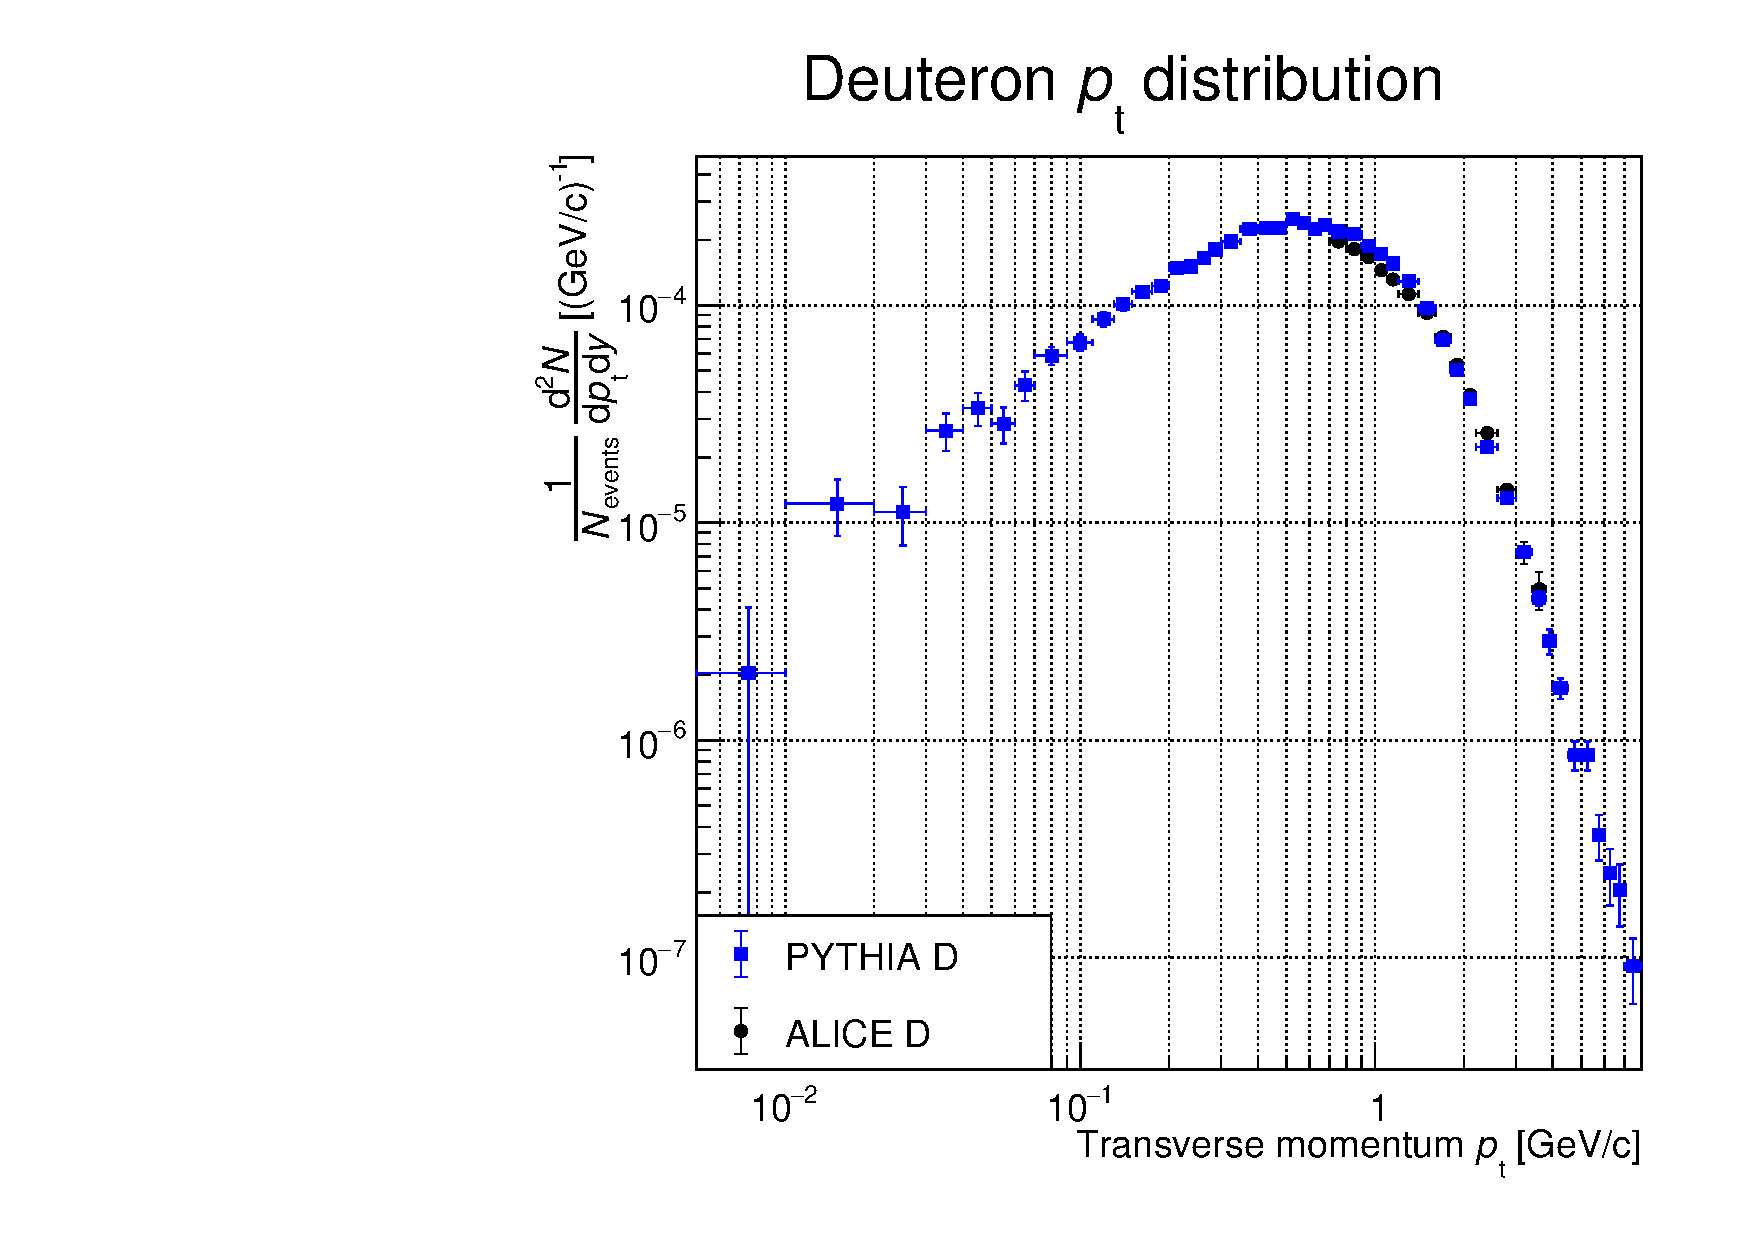
\includegraphics[width=\textwidth]{image/3-risultati/analyse/G/deuteron.pdf}
        \caption{}
        \label{fig:D_deuteron}
    \end{subfigure}
    %\hspace{1cm}
    \begin{subfigure}{.49\textwidth}
        \centering
        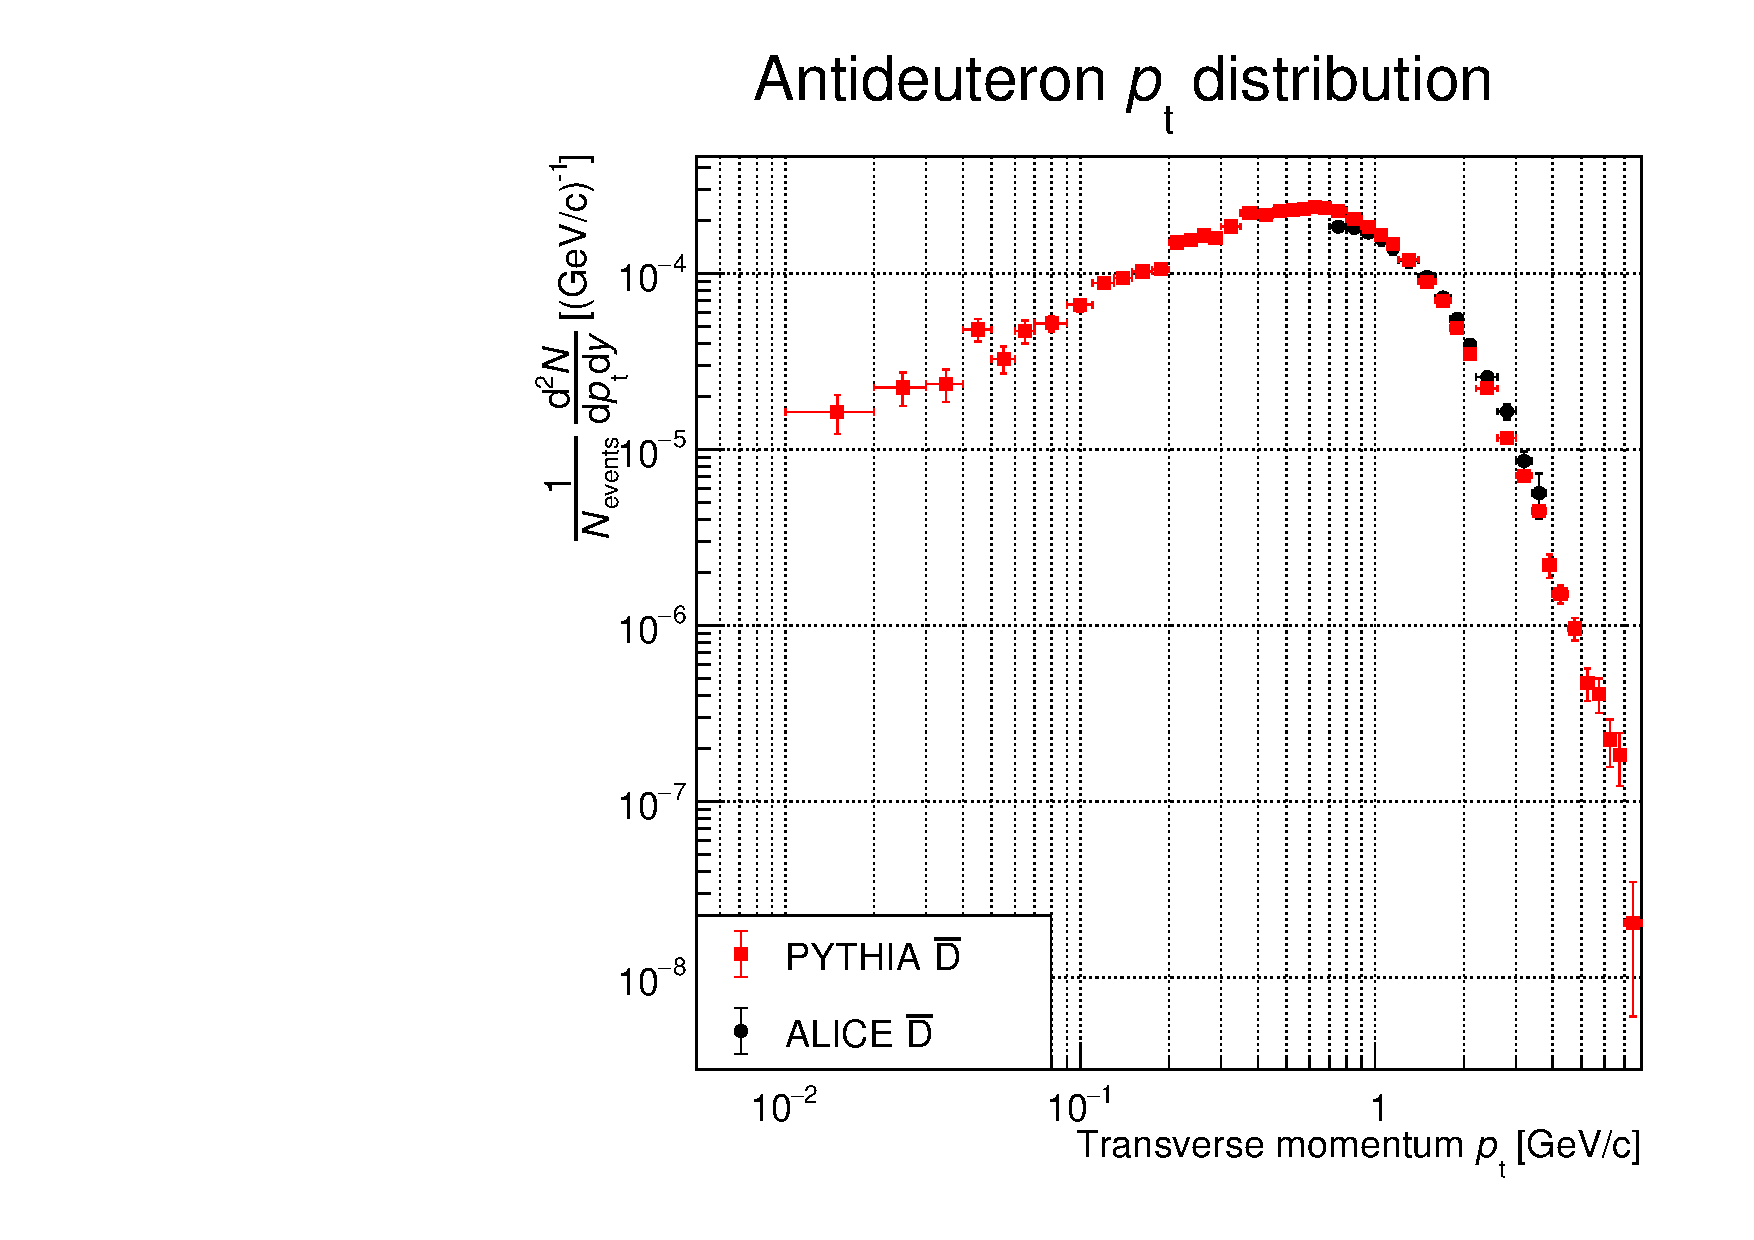
\includegraphics[width=\textwidth]{image/3-risultati/analyse/G/antideuteron.pdf}
        \caption{}
        \label{fig:D_antideuteron}
    \end{subfigure}
    \captionwithsource{Distribuzione dell'impulso trasverso di \emph{\rmfamily (a)} $D$ e \emph{\rmfamily (b)} di $\bar D$ in confronto con i dati di ALICE, utilizzando il modello ottimizzato.}{\cite{ALICE:2020foi}}
    \label{fig:D_(anti)deuteron}
\end{figure}
\begin{figure}[htp]
    \centering
    \begin{subfigure}{.49\textwidth}
    \centering
        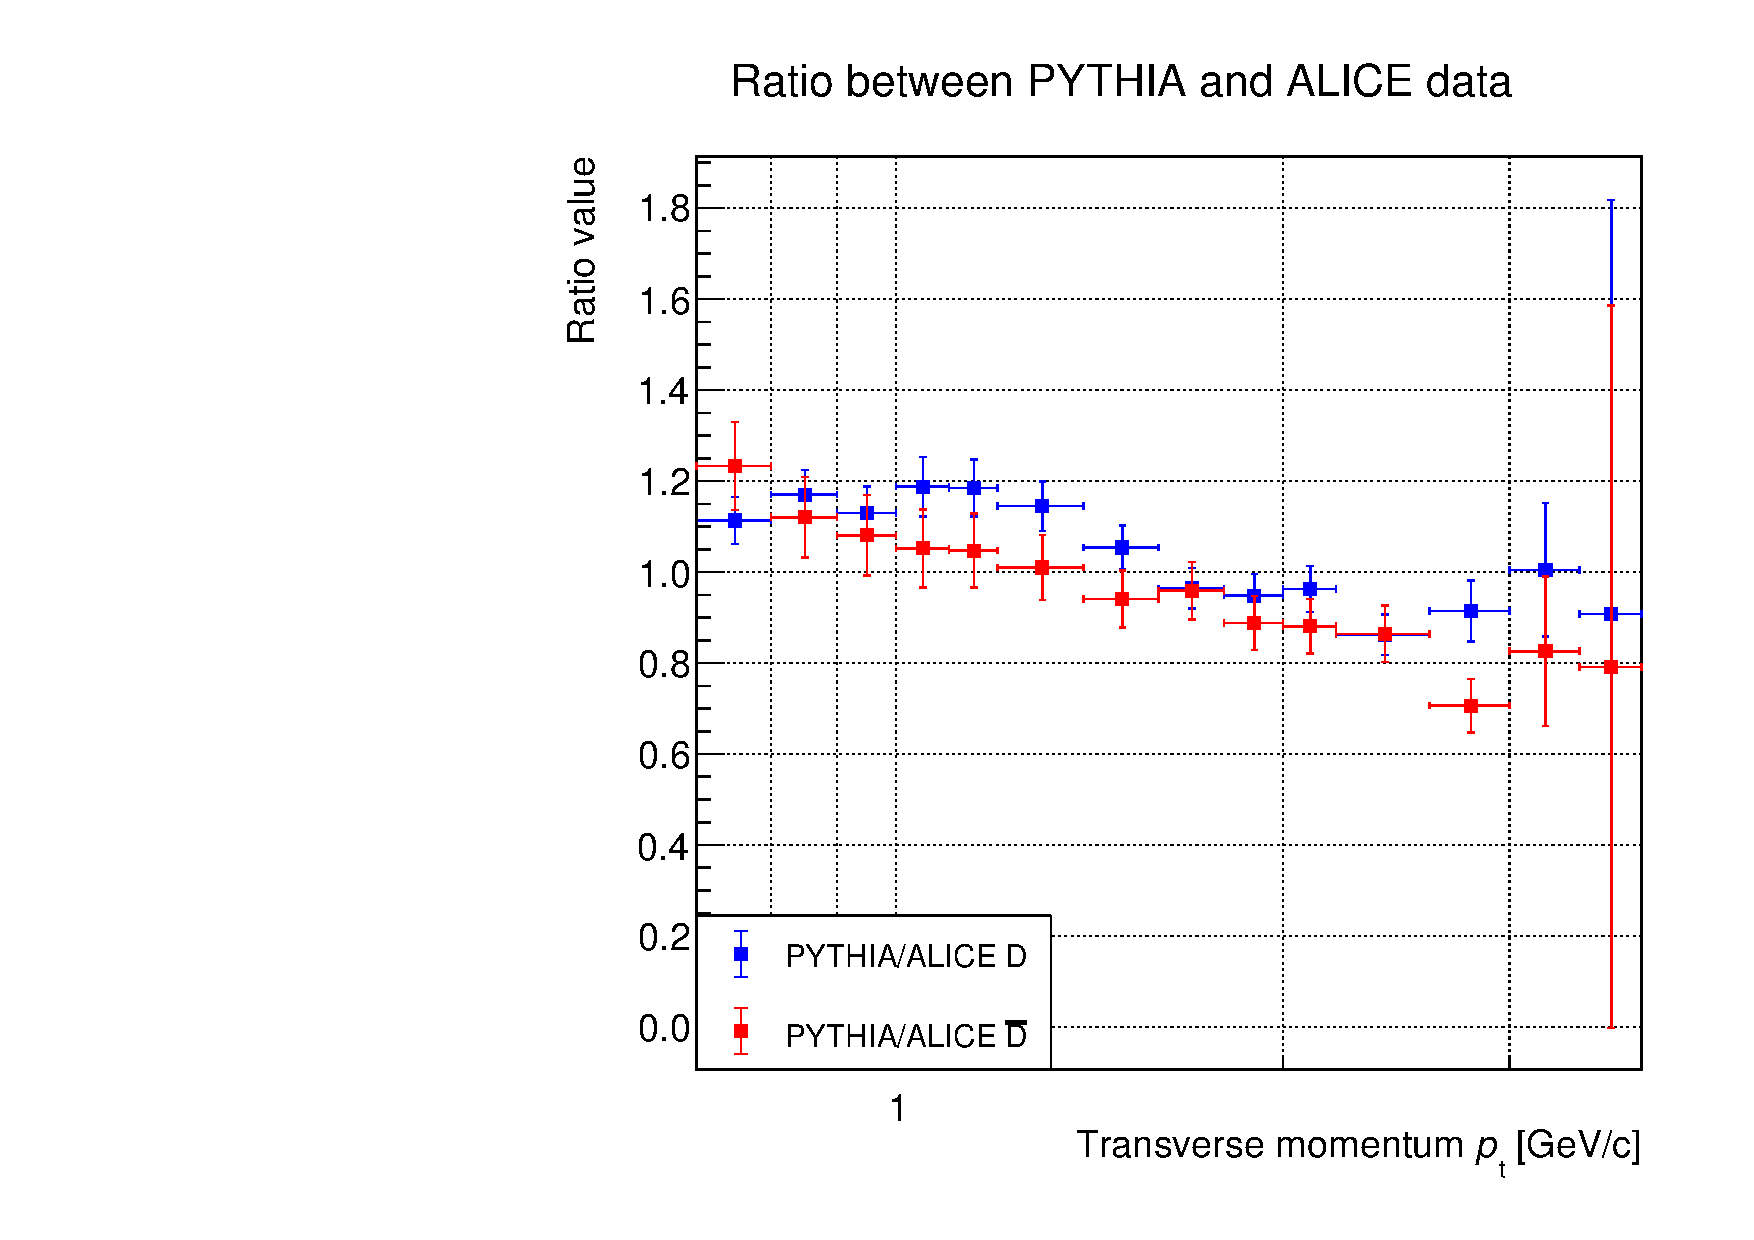
\includegraphics[width=\textwidth]{image/3-risultati/analyse/G/division.pdf}
        \caption{}
        \label{fig:D_division}
    \end{subfigure}
    %\hspace{1cm}
    \begin{subfigure}{.49\textwidth}
        \centering
        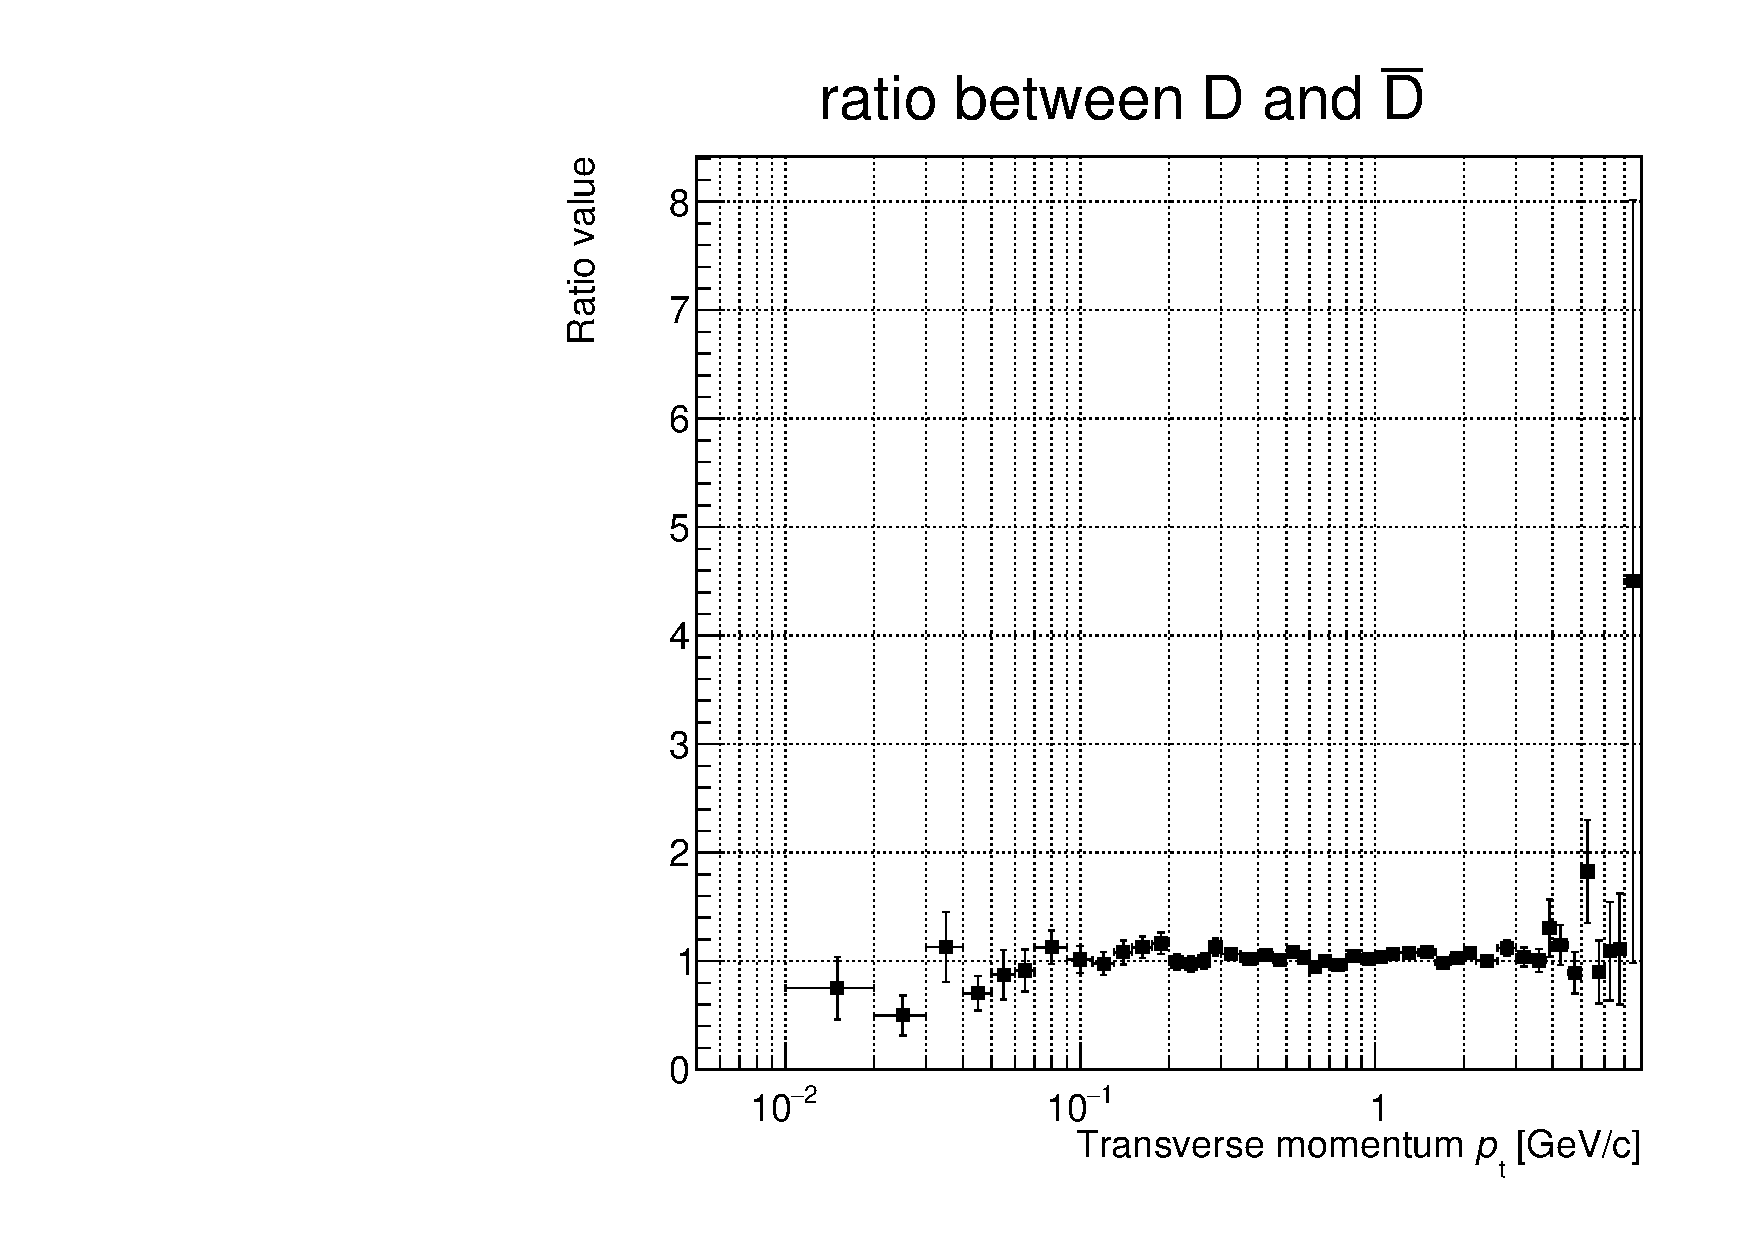
\includegraphics[width=\textwidth]{image/3-risultati/analyse/G/ratio_DD.pdf}
        \caption{}
        \label{fig:D_ratio_DD}
    \end{subfigure}
    \caption{\emph{\rmfamily (a)} Divisione tra la distribuzioni dell'impulso trasverso di $D$ e $\bar D$ con i dati di ALICE, utilizzando il modello ottimizzato. \emph{\rmfamily (b)} Frazione delle distribuzione dell'impulso trasverso di $D$ con quello di $\bar D$, utilizzando il modello ottimizzato.}
    \label{fig:D_ratio_DD_}
\end{figure}
\begin{figure}[h]
    \centering
    \begin{subfigure}{.49\textwidth}
    \centering
        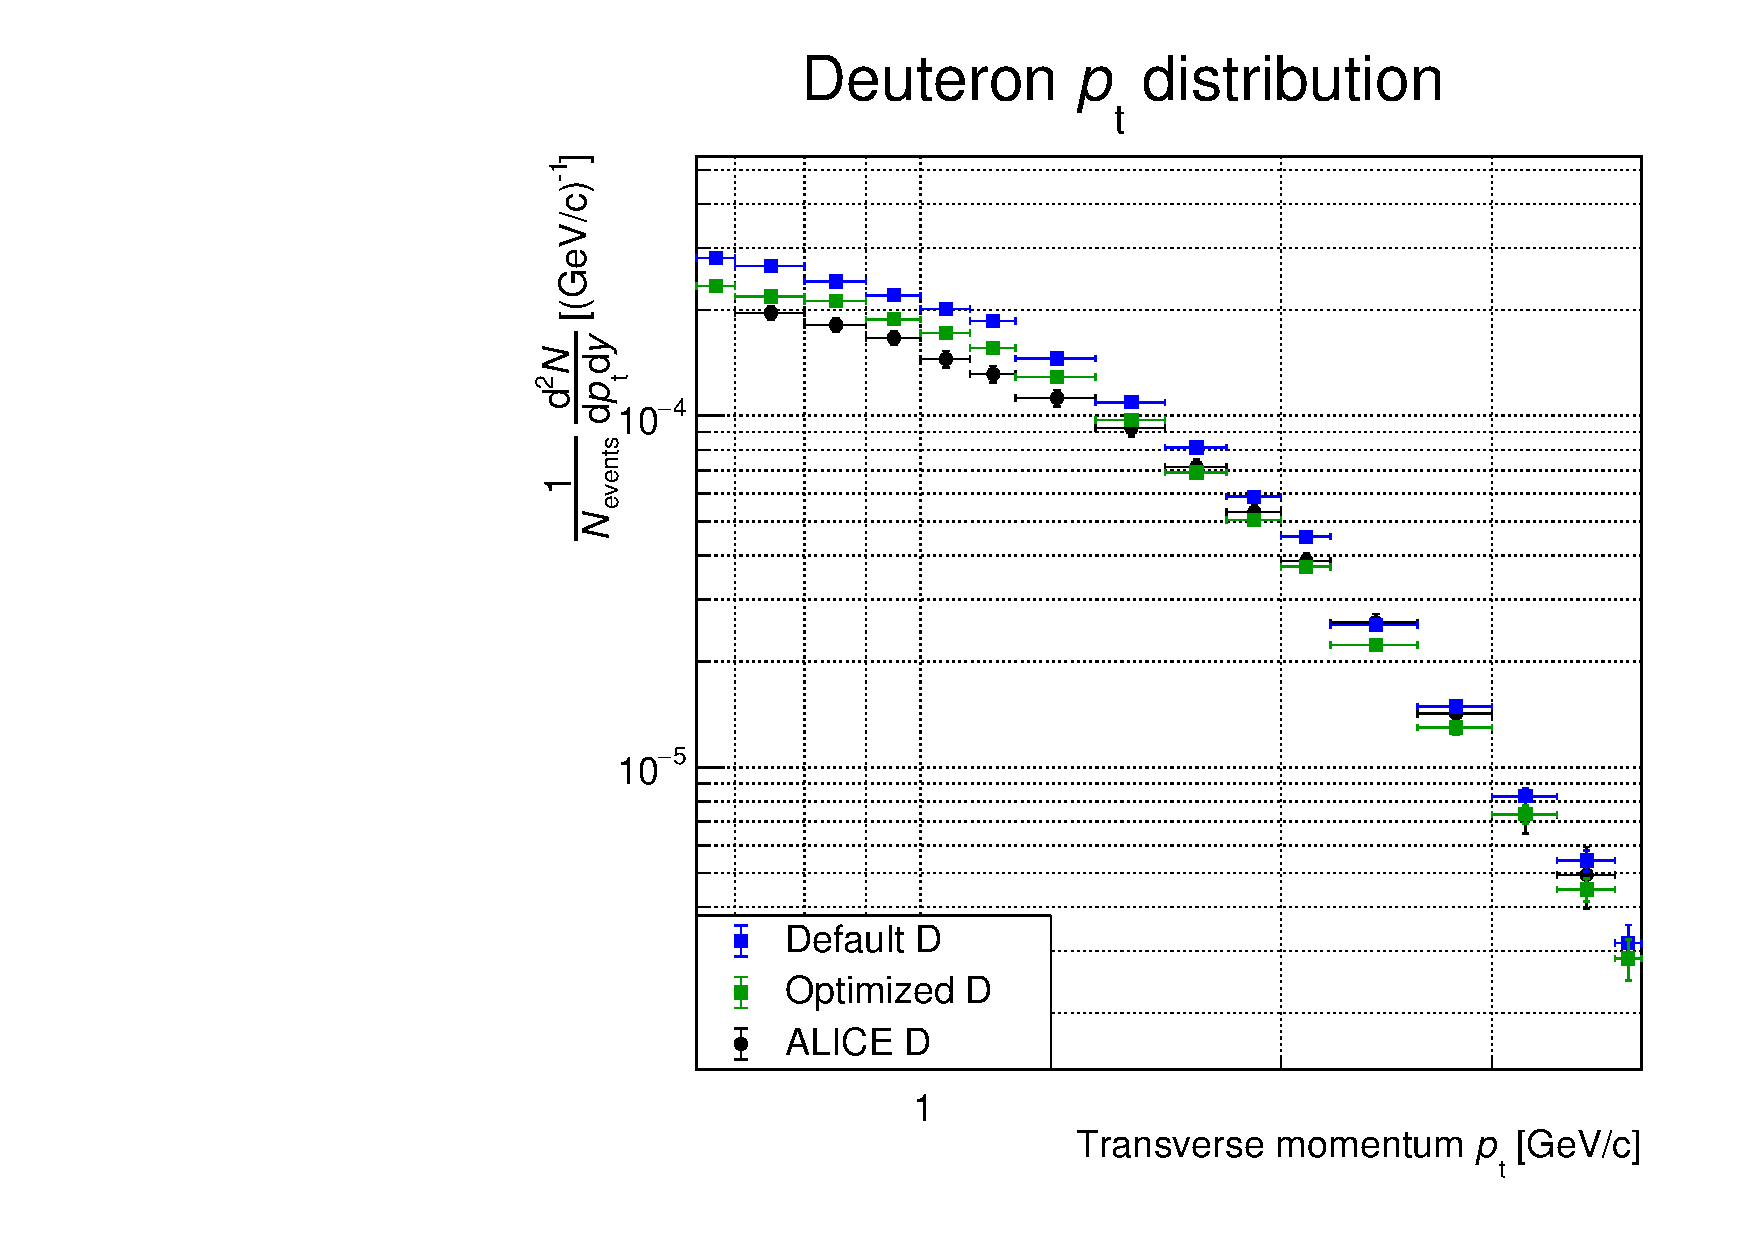
\includegraphics[width=\textwidth]{image/3-risultati/analyse/G/def_opt_deuteron.pdf}
        \caption{}
        \label{fig:def_opt_deuteron}
    \end{subfigure}
    %\hspace{1cm}
    \begin{subfigure}{.49\textwidth}
        \centering
        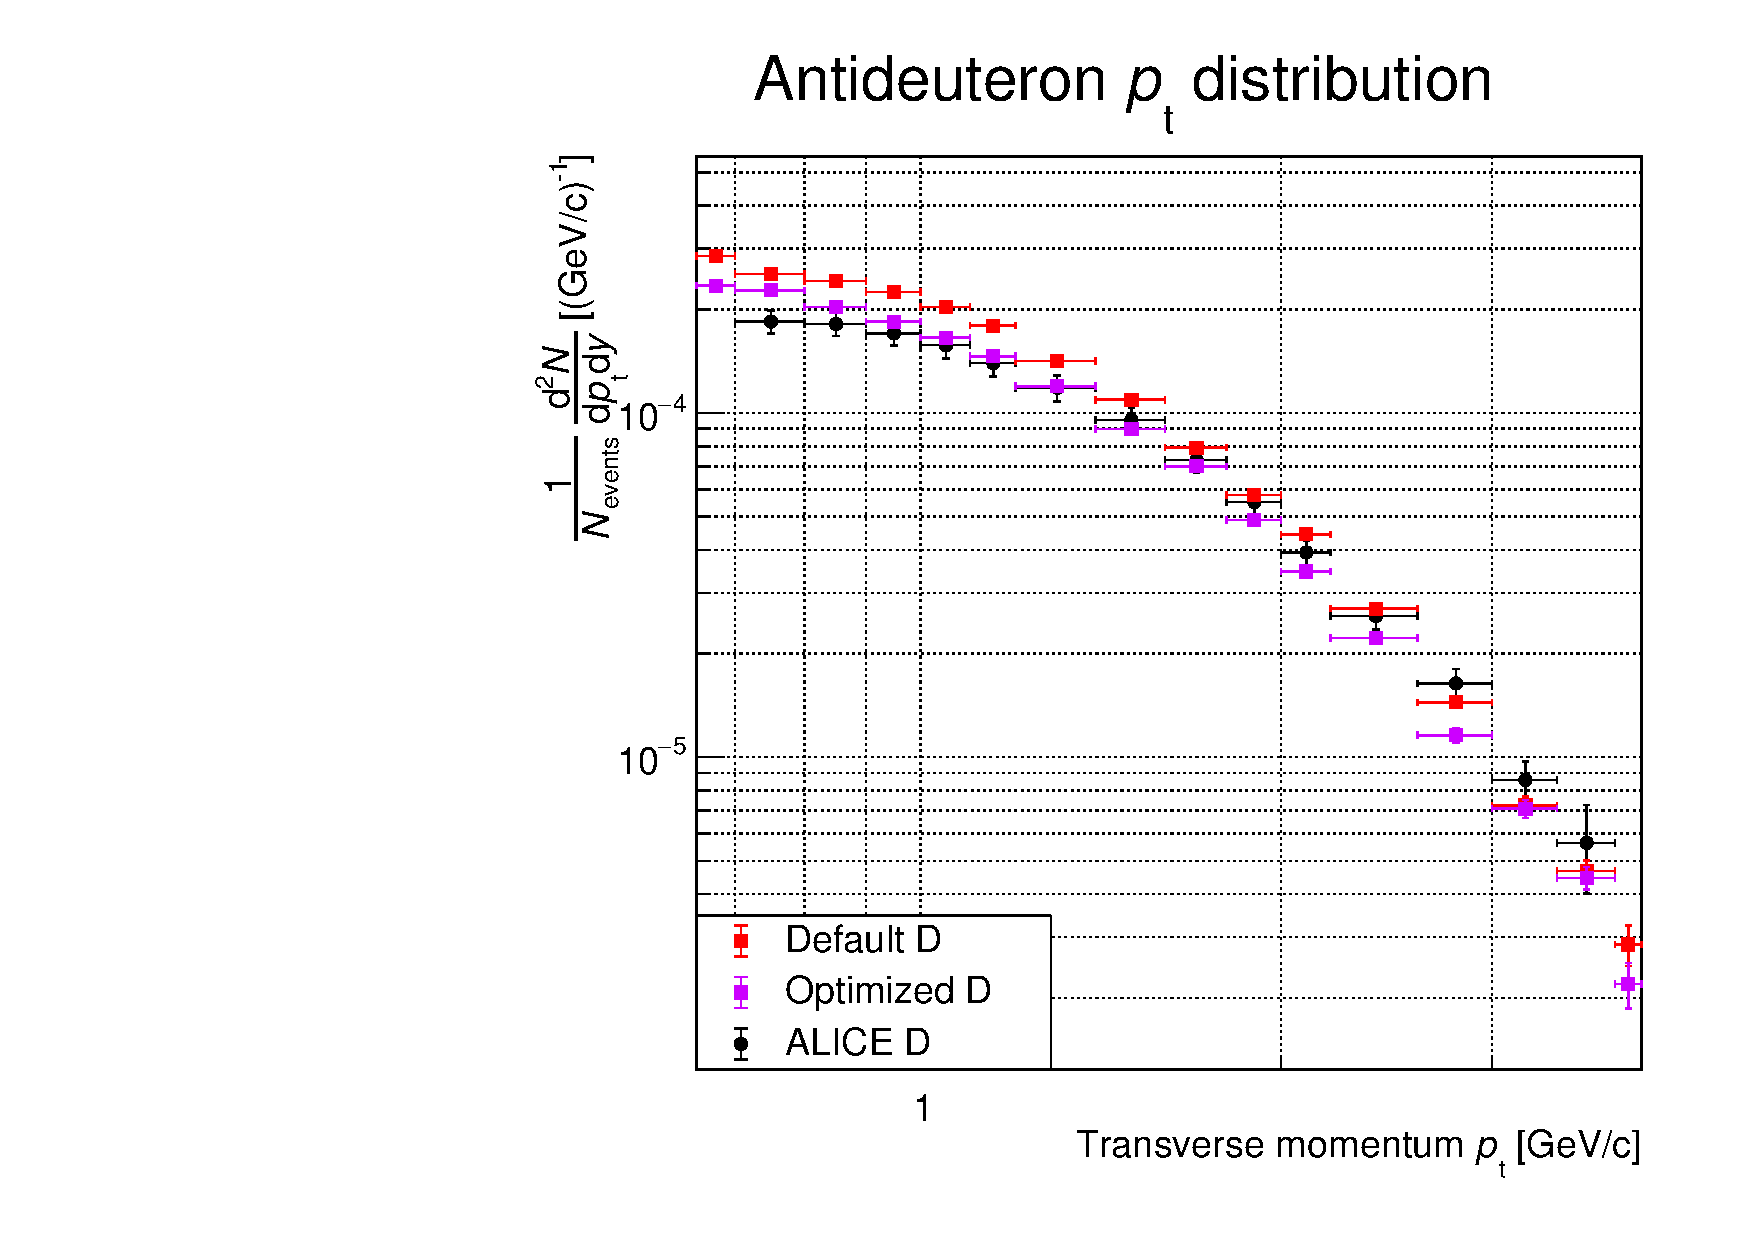
\includegraphics[width=\textwidth]{image/3-risultati/analyse/G/def_opt_antideuteron.pdf}
        \caption{}
        \label{fig:def_opt_antideuteron}
    \end{subfigure}
    \captionwithsource{Distribuzioni dell'impulso trasverso dei deuteroni e dei antideuteroni del modello predefinito ("Default"), ottimizzato ("Optimized") e dei dati di ALICE.}{\cite{ALICE:2020foi}} 
    \label{fig:def_opt}
\end{figure}